\Opensolutionfile{ans}[appendices/vastaukset]

\chapter{Polynomi}
	\section{Peruskäsitteitä}

\qrlinkki{http://opetus.tv/maa/maa2/polynomien-peruskasitteet/}
{Opetus.tv: \emph{polynomien peruskäsitteet} (9:00)}

\qrlinkki{http://opetus.tv/maa/maa2/polynomin-tasmallinen-maaritelma/}
{Opetus.tv: \emph{polynomin täsmällinen määritelmä} (6:10)}

\subsection*{Polynomit}

\termi{polynomi}{Polynomit} ovat matematiikassa tärkeitä lausekkeita.

\laatikko{Polynomi on lauseke, jossa esiintyy vain:
\begin{itemize}
\item muuttujien potensseja (eksponentti luonnollinen luku, mukaan lukien $0$)
\item kerrottuna jollakin vakiolla sekä
\item näiden potenssitermien summia.
\end{itemize}
}

Polynomissa voi olla yksi tai useampia muuttujia, tai se voi olla muuttujaton vakiopolynomi. Vakiopolynomin tapauksessa muuttujan eksponentin ajatellaan olevan $0$, sillä $x^0=1$, jolloin muuttuja katoaa.

\begin{esimerkki}
Kaikki seuraavat lausekkeet ovat polynomeja:

\begin{tabular}{ll}
$4$ &  ei muuttujia ($4x^0=4 \cdot 1=4$)\\
$2x+1$ &  muuttujana $x$ ($x^1=x$)\\
$5x^2+x-7$ &   muuttujana $x$\\
$-3t^{100}$& muuttujana $t$\\
$y$& muuttujana $y$\\
$y^2+1$& muuttujana $y$\\
$xy^2+x^2y$& muuttujina $x$ ja $y$
\end{tabular}

\end{esimerkki}

\begin{esimerkki}

Miksi muuttujan $t$ lausekkeet 
\begin{enumerate}
\item $\frac{2}{t}$
\item $\pi^t$
\item $\sqrt{t}+2$ ja
\item $t^\pi$
\end{enumerate}

\emph{eivät ole} polynomeja?

	\begin{esimratk}

\begin{enumerate}
\item $\frac{2}{t}$ ei ole polynomi, sillä muuttujan $t$ eksponentti ei ole luonnollinen luku: $\frac{2}{t}=2 \cdot \frac{1}{t}= 2t^{-1}$, ja $-1 \notin \mathbb{N}$.
\item $\pi^t$ ei ole polynomi, sillä muuttuja on eksponentissa eikä potenssin kantalukuna.
\item $\sqrt{t}+2$ ei ole polynomi, sillä neliöjuuri ei ole esitettävissä potenssina, jonka eksponentti olisi luonnollinen luku: $\sqrt{t}+2=t^{\frac{1}{2}}+2$, ja $-2 \notin \mathbb{N}$.
\item $t^{\pi}$ ei ole polynomi, sillä muuttujan eksponentti ei ole luonnollinen luku: $\pi \notin \mathbb{N}$.
\end{enumerate}

	\end{esimratk}
\end{esimerkki}

Polynomi on summalauseke, joiden yhteenlaskettavia kutsutaan \termi{termi}{termeiksi}. Termejä edeltävät miinukset ymmärretään termin osaksi negatiivisina kertoimina. Esimerkiksi polynomin $-2x^3+5x^2+x-7$ termit ovat $-2x^3$, $5x^2$, $x$ ja $-7$. Termejä, jotka eivät sisällä muuttujaa, kutsutaan  \termi{vakiotermi}{vakiotermeiksi}. Vakiotermejä ovat siis esimerkiksi $1$, $-7$, $\frac{\pi}{2}$ ja $-\sqrt{2}$.

%etymologiahuomautukset sivun laitaan?

Polynomi-sanan 'poly' on kreikkaa ja tarkoittaa montaa. Erityisesti yhden termin polynomeja kutsutaan \termi{monomi}{monomeiksi}, kahden termin polynomeja \termi{binomi}{binomeiksi}, kolmen termin polynomeja \termi{trinomi}{trinomeiksi} ja niin edelleen:
\begin{center}\begin{tabular}{ccc}
monomi	& binomi 	&	trinomi \\
$-3x^2$   &	$x^2-5$	& $y^2+3y-x$
 \end{tabular} \end{center}

Muuttujan eksponenttia kutsutaan termin \termi{aste}{asteeksi} tai \termi{asteluku}{asteluvuksi}. Vakiotermin aste on nolla. \termi{Polynomin aste}{Polynomin aste} on suurin sen sievennetyn muodon termien asteista. Polynomin asteen saaminen selville voi vaatia polynomin sieventämistä. Esimerkiksi $x^2-x^2+1$ ei ole toisen, vaan nollannen asteen polynomi, sillä sievennettynä $x^2-x^2+1=1$. (Ja $1=1x^0$.) Useamman muuttujan tapauksessa polynomin termien asteet lasketaan muuttujien potenssien summana.

\begin{esimerkki}
    Mitkä ovat polynomin $x^4-2x^3+5$ termit ja niiden asteet? Mikä on polynomin aste?
    \begin{esimvast}
        Polynomin $x^4-2x^3+5$ termit ovat $x^4$, $-2x^3$ ja $5$ ja niiden asteet ovat
        neljä, kolme ja nolla. Polynomin aste on sama kuin sama kuin
        korkein termien asteista, eli neljä.
    \end{esimvast}
\end{esimerkki}

Koska yhteenlasku on vaihdannainen, polynomin termit voi kirjoittaa missä tahansa järjestyksessä. Esimerkiksi polynomi $y^4+y^2-1$ voidaan kirjoittaa myös järjestyksessä $-1+y^4+y^2$. Yleensä polynomien termit kirjoitetaan niiden asteen perusteella laskevaan järjestykseen niin, että korkeimman asteen termi kirjoitetaan ensin. Useaa muuttujaa sisältävät termit on tapana kirjoittaa ennen yhtä muuttujaa sisältäviä termejä – kuitenkin niin, että potenssijärjestys on tärkeämpi.

\begin{esimerkki}
	Mikä on polynomin $3t^2-1+t^3$ aste? Mikä on korkeimman asteen termin kerroin?
\begin{esimratk}
	
Aloitetaan järjestämällä polynomin termit asteluvun mukaiseen laskevaan järjestykseen: \\
	  $\textcolor{blue}{3t^2}\textcolor{red}{-1}+t^3=$ \\
	  $t^3\textcolor{blue}{+3t^2}\textcolor{red}{-1}$ \\
	
\end{esimratk}

\begin{esimvast}
Polynomi on kolmatta astetta. Korkeimman (eli kolmannen) asteen termin kerroin on $1$.
\end{esimvast}

\end{esimerkki}

\begin{esimerkki}
	Kuinka monetta astetta on (kahden muuttujan) polynomi $x^2+2xy^2+xy$?
\begin{esimratk}
Merkitään selkeyden vuoksi molempien muuttujien kaikkien eksponentit näkyviin: \\
\[x^2+2x^1y^2+x^1y^1\]

Kun termissä on kaksi eri muuttujaa, niin termin asteluku on näiden muuttujien eksponenttien summa. Näin ollen ensimmäisen termin aste on kaksi, toisen termin aste on $1+2=3$ ja kolmannen termin aste on $1+1=2$. Järjestetään termit vielä asteiden mukaiseen laskevaan järjestykseen:

\[\textcolor{blue}{x^2}+\textcolor{red}{2x^1y^2}+x^1y^1\]
\[\textcolor{red}{2x^1y^2}+x^1y^1+\textcolor{blue}{x^2}\]

\end{esimratk} 

\begin{esimvast}
Polynomin asteluku on kolme.
\end{esimvast}

\end{esimerkki}

\subsection*{Polynomifunktion arvo}

\qrlinkki{http://opetus.tv/maa/maa2/polynomiesimerkkeja/}
{Opetus.tv: \emph{polynomiesimerkkejä} (6:59 ja 7:43)}

Polynomi reaalilukujen laskutoimituksena määrittää funktion, jota kutsutaan \termi{polynomifunktio}{polynomifunktioksi}. Oletusarvoisesti kaikkien lukiomatematiikassa käsiteltävien polynomifunktioiden määrittelyjoukko on koko reaalilukujen joukko $\mathbb{R}$, ja tällöin myös funktion arvot reaalilukuja. (Numeeristen ja algebrallisten menetelmien syventävällä kurssilla tarkastellaan polynomifunktioita myös reaalilukujoukkoa laajemmalla kompleksilukualueella $\mathbb{C}$.)

Polynomifunktioita nimetään tyypillisesti suuraakkosin kuten $P$, $Q$ tai $R$.

\begin{esimerkki}

Polynomi $5x^2-3x+2$ määrittää funktion $P:\mathbb{R}\rightarrow \mathbb{R}$, jonka arvot voidaan laskea kaavalla $P(x)=5x^2-3x+2$. Arvoja voidaan laskea siis sijoittamalla joitakin (mielivaltaisia) lukuja muuttujan $x$ paikalle:
\begin{align*}
    P(\textcolor{blue}{2}) & = 5\cdot \textcolor{blue}{2}^2-3\cdot \textcolor{blue}{2}+2 = 20 - 6 + 2 = 16 \\
    P(\textcolor{blue}{-1}) & = 5(\textcolor{blue}{-1})^2-3(\textcolor{blue}{-1})+2 = 5 + 3 + 2 = 10 \\
    P(\textcolor{blue}{-3}) & = 5(\textcolor{blue}{-3})^2-3(\textcolor{blue}{-3})+2 = 45 + 9 + 2 = 56.
\end{align*}
\end{esimerkki}

Polynomeja ja polynomifunktioita käsitellään usein yhtäläisesti; voidaan esimerkiksi sanoa ''polynomi $P(x)=2x+1$'', vaikka tarkoitetaan vastaavaa polynomifunktiota.

%pitäisikö täsmentää? ^

\subsection*{Polynomien yhteen- ja vähennyslasku}

\qrlinkki{http://opetus.tv/maa/maa2/polynomien-yhteen-ja-vahennyslasku/}
{Opetus.tv: \emph{polynomien yhteen- ja vähennyslasku} (7:36)}

Polynomien summat ja erotukset ovat aina polynomeja. Polynomeja voidaan laskea yhteen yhdistämällä samanasteiset termit. On kätevää aloittaa ryhmittelemällä samanasteiset termit vierekkäin. 

Samanasteisten termien yhteen- ja vähennyslasku perustuu siihen, että soveltamalla reaalilukujen osittelulakia $a(b\pm c)=ab\pm ac$ oikealta vasemmalle (ks. Vapaa matikka 1) samanasteiset potenssit voidaan ottaa yhteiseksi tekijäksi:

\[ ax^n+bx^n = (a+b)x^n \]

\begin{esimerkki}

	\begin{itemize}
	\item $2x+3x=(2+3)x=5x$
	\item $T-5T=1T-5T=(1-5)T$
	\item $5x^2+3x^2 = (5+3)x^2 = 8x^2$
	\item $\frac{1}{2}y^{42}+\frac{1}{3}y^{42}=(\frac{1}{2}+\frac{1}{3})y^{42}= \\
	(\frac{3}{6}+\frac{2}{6})y^{42}=\frac{3+2}{6}y^{42}=\frac{5}{6}y^{42}$
	\end{itemize}
\end{esimerkki}

\begin{esimerkki}
Laske polynomien $5x^2-x+5$ ja $3x^2-1$ summa.
    \begin{esimratk}
        \begin{align*}
            (\textcolor{blue}{5x^2} \textcolor{red}{{}-x} + 5) + (\textcolor{blue}{3x^2} -1) 
            &=\textcolor{blue}{5x^2} \textcolor{red}{{}-x} + 5 + \textcolor{blue}{3x^2} -1 \\
            &=\textcolor{blue}{5x^2+3x^2} \textcolor{red}{{}-x} +5-1\\
%                       &=\textcolor{blue}{(5+3)x^2} \textcolor{red}{{}-x}+(5-1)\\
            &=\textcolor{blue}{8x^2} \textcolor{red}{{}-x}+4.
        \end{align*}
    \end{esimratk}
    \begin{esimvast}
        Polynomien summa on $8x^2-x+4$.
    \end{esimvast}
\end{esimerkki}

Polynomeja voidaan vastaavalla tavalla vähentää toisistaan. (Kun sulkujen edessä on miinusmerkki, tulee muistaa vaihtaa termien merkit sulkuja avattaessa.)

\begin{esimerkki}
    Laske polynomien $4x^3+1$ ja $6x^3-2$ erotus.
    \begin{esimratk}
        \begin{align*}
		(\textcolor{blue}{4x^3}+1)-(\textcolor{blue}{6x^3}-2) \\
		&= \textcolor{blue}{4x^3}+1 - \textcolor{blue}{6x^3} -(-2) \\
		&= \textcolor{blue}{4x^3}+1 - \textcolor{blue}{6x^3} + 2 \\
		&= \textcolor{blue}{4x^3-6x^3} +1 +2 \\
		&=\textcolor{blue}{-2x^3}+3
        \end{align*}
    \end{esimratk}
    \begin{esimvast}
        Polynomien erotus on $-2x^3+3$.
    \end{esimvast}
\end{esimerkki}

\begin{esimerkki}
    Laske polynomien $14x^3+69$ ja $3x^3+2x^2+x$ erotus.
    \begin{esimratk}
        \begin{align*}
            (\textcolor{blue!30!green}{14x^3} + 69) - (\textcolor{blue!30!green}{3x^3} \textcolor{blue}{{}+ 2x^2} \textcolor{red}{{}+x})
            &= \textcolor{blue!30!green}{14x^3} + 69 \textcolor{blue!30!green}{{}-3x^3} \textcolor{blue}{-2x^2} \textcolor{red}{{}-x} \\
            &= \textcolor{blue!30!green}{14x^3{}-3x^3} \textcolor{blue}{{}-2x^2} \textcolor{red}{{}-x} + 69 \\
%           &= \textcolor{blue!30!green}{(14{}-3)x^3} \textcolor{blue}{{}-2x^2} \textcolor{red}{{}-x} + 69 \\
            &= \textcolor{blue!30!green}{11x^3} \textcolor{blue}{{}-2x^2} \textcolor{red}{{}-x} + 69
        \end{align*}
    \end{esimratk}
    \begin{esimvast}
        Polynomien erotus on $11x^3-2x^2-x+69$.
    \end{esimvast}
\end{esimerkki}

\begin{esimerkki}
    Olkoot polynomit $P(x)=2x+1$ ja $Q(x)=3x^2-2x+5$. Määritä summa $R(x)=P(x)+Q(x)$.
    \begin{esimratk}
        \begin{align*}
            R(x) = P(x)+Q(x) &= (2x+1)+(3x^2-2x+5) \\
                             &= 2x+1+3x^2-2x+5 \\
                             &= 3x^2+2x-2x+1+5 \\
                             &= 3x^2+6.
        \end{align*}
    \end{esimratk}
    \begin{esimvast}
        $R(x) = 3x^2+6$.
    \end{esimvast}
\end{esimerkki}

\begin{esimerkki}
    Laske polynomien $P$ ja $Q$ erotus $R$, kun $P(x)=-3x^4+x^2+1$ ja $Q(x)=-3x^4+3x^3-x$.
    Mikä on polynomin $R$ aste?
   \begin{esimratk}
        \begin{align*}
            R(x) = P(x)-Q(x) &= (-3x^4+x^2+1)-(-3x^4+3x^3-x) \\
                             &= -3x^4+x^2+1+3x^4-3x^3+x \\
                             &= -3x^4+3x^4-3x^3+x^2+x+1 \\
                             &= -3x^3+x^2+x+1.
        \end{align*}
    \end{esimratk}
    \begin{esimvast}
        $R(x) = -3x^3+x^2+x+1$. Polynomin $R$ aste on kolme.
    \end{esimvast}
\end{esimerkki}

\subsection*{Polynomin yleinen muoto}

Polynomit sievennetään yleensä yleiseen muotoon, jossa on vain yksi termi kutakin astetta kohti.

Formaalisti kirjoitettuna yhden muuttujan polynomin yleinen muoto on
\[a_n x^n + a_{n-1} x^{n-1} + \ldots + a_1 x + a_0 \] 
jollakin $n\in\N$. Muuttuja $n$ kertoo polynomin asteen, ja kertoimet $a_0, a_1, \ldots, a_{n-1}, a_n$ ovat reaalilukuvakioit. Kertoimen symbolilla $a$ on juoksevana alaindeksinä sama luku $n$ siksi, että vakioita on yhtä monta kuin on polynomin aste. Jos jokin kertoimista on $0$, kyseinen termi katoaa nollan kertolaskuominaisuuksien vuoksi..

\begin{esimerkki}

Polynomi $-3x^{13}-\frac{3}{4}x^2-17$ on polynomin yleistä muotoa siten, että $n=13$, $a_{13}=-3$, $a_2=-\frac{3}{4}$ ja $a_0=-17$, ja kaikki muut kertoimet ovat nollia.

\end{esimerkki}
 
Jokainen lauseke, joka on esitettävissä polynomin yleisessä muodossa, on polynomi.

\begin{esimerkki}

Lauseke $\frac{2x^2+1}{x}$ ei ensi näkemältä näytä polynomilta murtolausekkeen nimittäjässä olevan $x$:n vuoksi. Lauseketta on kuitenkin mahdollista sieventää esimerkiksi seuraavasti: \\


$\frac{2x^3+x^2}{x} = \frac{2x^3}{x}+\frac{x^2}{x} = 2x^2+x $ \\

Kyseessä oli siis kuitenkin toisen asteen kaksiterminen yhden muuttujan polynomi. (Huomataan kuitenkin, että alkuperäisen esitysmuodon vuoksi $x \neq 0$, koska nollalla jakamista ei ole määritelty.)

\end{esimerkki}

\begin{tehtavasivu}

\paragraph*{Opi perusteet}

\begin{tehtava}
    Mitkä seuraavista ovat polynomeja?
    \begin{enumerate}[a)]
        \item $\frac{1}{x}$
       %\item $x^3+4x$
        \item $5x-125$
       %\item $2^x$
        \item $\sqrt{x}+1$
        \item $3x^4+6x^2+9$
        \item $\sqrt{2}x-x$
        \item $4^x+5x+6$
    \end{enumerate}
    \begin{vastaus}
        \begin{enumerate}[a)]
            \item Ei ole.
           %\item On.
            \item On.
           %\item Ei ole.
            \item Ei ole.
            \item On.
            \item On.
            \item Ei ole.
        \end{enumerate}
    \end{vastaus}
\end{tehtava}

\begin{tehtava}
	Mikä on/mitkä ovat polynomin \\ $P(x) = x^5-3x^3+2x-1$
	\begin{enumerate}[a)]
		\item aste
		\item termit
		\item kolmannen asteen termi
		\item kolmannen termin aste
		\item vakiotermi
	\end{enumerate}

	\begin{vastaus}
		\begin{enumerate}[a)]
			\item $5$
			\item $x^5$, $-3x^3$, $2x$, $-1$
			\item $-3x^3$
			\item $1$
			\item $-1$
		\end{enumerate}
	\end{vastaus}
\end{tehtava}


\begin{tehtava}
    Täydennä taulukko. Polynomeissa on vain yksi muuttuja, $x$.
        
    \begin{tabular}{|c|c|c|c|c|}
                                                                         \hline
polynomi     & \begin{sideways}\begin{minipage}{3.5cm}termien\\lukumäärä\end{minipage}\end{sideways}%
& \begin{sideways}\begin{minipage}{3.5cm}korkeimman asteen\\termin kerroin\end{minipage}\end{sideways}%
& \begin{sideways}\begin{minipage}{3.5cm}polynomin\\asteluku\end{minipage}\end{sideways}%
& \begin{sideways}vakiotermi\end{sideways} \\ \hline
$-2x^2+6x$   &        2  &         $-2$      &       2   &    0       \\ \hline 
$7x^3-x-15$  &           &                   &           &            \\ \hline 
             &        2  &          $-9$     &       2   &    5       \\ \hline 
%             &        3  &          $-1$     &       5   &    $-17$   \\ \hline 
%             &        4  &                   &       3   &            \\ \hline 
             &        1  &          -5       &       99  &            \\ \hline                           
    \end{tabular}

%      \begin{tabular}{|l|c|c|c|c|c|c|}
%                                                                                            \hline
% polynomi     & \begin{sideways}$-2x^2+6x$\end{sideways} & \begin{sideways}$7x^3-x-15$\end{sideways}    &     &          &     &     \\ \hline
% termien      &            &                &     &          &     &     \\ \hline 
% lukumäärä    &        2   &                & 2   &    3     &  4  &  1  \\ \hline 
% korkeimman & & & & & & \\  
% asteen & & & & & & \\  
% termin & & & & & & \\  
% kerroin      &    $-2$    &                &$-9$ &   $-1$   &     &$-5$ \\ \hline 
% polynomin & & & & & & \\  
% asteluku     &        2   &                & 2   &    5     &  3  & 99  \\ \hline 
% vakiotermi   &        0   &                & 5   &    $-17$ &     &     \\ \hline 
%     \end{tabular}
%      \begin{tabular}{|c|c|c|c|c|}
%                                                                                           \hline
%              & termien   & korkeimman asteen & polynomin &            \\
% polynomi     & lukumäärä & termin kerroin    & asteluku  & vakiotermi \\ \hline
% $-2x^2+6x$   &        2  &         $-2$      &       2   &    0       \\ \hline 
% $7x^3-x-15$  &           &                   &           &            \\ \hline 
%              &        2  &          $-9$     &       2   &    5       \\ \hline 
%              &        3  &          $-1$     &       5   &    $-17$   \\ \hline 
%              &        4  &                   &       3   &            \\ \hline 
%              &        1  &          -5       &       99  &            \\ \hline                           
%     \end{tabular}

    
    \begin{vastaus}

	    \begin{tabular}{|c|c|c|c|c|}
                                                                                           \hline
polynomi     & \begin{sideways}\begin{minipage}{3.5cm}termien\\lukumäärä\end{minipage}\end{sideways}%
& \begin{sideways}\begin{minipage}{3.5cm}korkeimman asteen\\termin kerroin\end{minipage}\end{sideways}%
& \begin{sideways}\begin{minipage}{3.5cm}polynomin\\asteluku\end{minipage}\end{sideways}%
& \begin{sideways}vakiotermi\end{sideways} \\ \hline
$-2x^2+6x$   &        2          &         $-2$      &       2             &    0       \\ \hline 
$7x^3-x-15$  &        3          &           7       &       3             &    $-15$   \\ \hline 
$-9x^2+5$    &        2          &          $-9$     &       2             &    5       \\ \hline 
%$-x^5\textcolor{blue}{+4x}-17$%
%             &        3          &          $-1$     &       5             &    $-17$   \\ \hline 
%$\textcolor{blue}{8}x^3\textcolor{blue}{-x^2+4x}-17$%
%             &        4          &\textcolor{blue}{8}  &       3             &\textcolor{blue}{17}\\ \hline 
$-5x^{99}$   &        1          &          $-5$     &       99            &         0      \\ \hline                           
   	  \end{tabular}
     \end{vastaus}
\end{tehtava}

\begin{tehtava}
    Sievennä.
    \begin{enumerate}[a)]
        \item $3x+5x $
        \item $4x^2+7x^2$
        \item $-6y+2y $
        \item $3x-(-2x)$
    \end{enumerate}
    \begin{vastaus}
        \begin{enumerate}[a)]
            \item $8x$
            \item $11x^2$
            \item $-4y$
            \item $5x$
        \end{enumerate}
    \end{vastaus}
\end{tehtava}

\begin{tehtava}
    Sievennä.
    \begin{enumerate}[a)]
    	\item $5x-2+2x+7$
        \item $5x-3y-y-2x$
        \item $2x^2+x+x^2-5x$
        \item $y^3 - 2y^2+4y^3-y $
    \end{enumerate}
    \begin{vastaus}
        \begin{enumerate}[a)]
        	\item $7x+5$
            \item $3x-4y$
            \item $3x^2-4x$
            \item $5y^3-2y^2-y$
        \end{enumerate}
    \end{vastaus}
\end{tehtava}

\begin{tehtava}
    Olkoot $P(x)=x^2+5$ ja $Q(x)=x^3-1$. Laske
    \begin{enumerate}[a)]
        \item polynomin $P(x)$ arvo, kun $x=2$
        \item polynomin $Q(x)$ arvo, kun $x=1$
        \item $P(-7)$
        \item $Q(-1)$.
    \end{enumerate}
    \begin{vastaus}
        \begin{enumerate}[a)]
            \item $9$ % 2^2 + 5 = 4 + 5 
            \item $0$ % 1^3 - 1
            \item $54$ % (-7)^2 + 5 = 49 + 5 
            \item $-2$ % (-1)^3 - 1 = -1 -1
        \end{enumerate}
    \end{vastaus}
\end{tehtava}

\paragraph*{Hallitse kokonaisuus}

\begin{tehtava}
    Sievennä.
    \begin{enumerate}[a)]
        \item $(x^2 - 2x + 1) + (-x^2 + x) $
        \item $(3y^3 + 2y^2  + y) - (-y^2 + y)$
        \item $(z^{10} - z^6 + z^2 + 1) + (z^{10} + 2z^8 - 3z^6)$
    \end{enumerate}
    \begin{vastaus}
        \begin{enumerate}[a)]
            \item $-x + 1$
            \item $3y^3 + 3y^2$
            \item $2z^{10} + 2z^8 - 4z^6 + z^2 + 1$
        \end{enumerate}
    \end{vastaus}
\end{tehtava}

\begin{tehtava}
	Mitkä ovat seuraavien polynomifunktioiden asteet, ts. sievennettyjen muotojen asteet?
	\begin{enumerate}[a)]
		\item $x+5-x$
		\item $x^2+x-2x^2$
		\item $4x^5+x^2-4-x^2$
		\item $x^4-2x^3+x-1+x^3-x^4+x^3$
	\end{enumerate}

	\begin{vastaus}
		\begin{enumerate}[a)]
			\item $0$
			\item $2$
			\item $5$
			\item $1$
		\end{enumerate}
	\end{vastaus}
\end{tehtava}

\begin{tehtava}
	Mitkä seuraavista polynomilausekkeista esittävät samaa polynomifunktiota kuin
	$x^3+2x+1$?
	\begin{enumerate}[a)]
		\item $2x+x^3+1$
		\item $x^2+2x+1$
		\item $x+2x^3+1 - (x^3+x)$
		\item $15+x^4+2x+x^3-x^4-14$
	\end{enumerate}
	\begin{vastaus}
		a) ja d)
	\end{vastaus}
\end{tehtava}

\begin{tehtava}
    Olkoot $P(x)=x^2+3x+4$ ja $Q(x)=x^3-10x+1$. Sievennä
    \begin{enumerate}[a)]
        \item $P(x)+Q(x)$
        \item $P(x)-Q(x)$
        \item $Q(x)-P(x)$
        \item $2P(3)+Q(2)$.
    \end{enumerate}
    \begin{vastaus}
        \begin{enumerate}[a)]
            \item $x^3+x^2-7x+5$ % x^2+3x+4 + x^3-10x+1
            \item $-x^3+x^2+13x+3$ % x^2+3x+4 -(x^3-10x+1) = x^2+3x+4 -x^3+10x-1
            \item $x^3-x^2-13x-3$ % 
            \item $33$ % 2*(3^2+3*3+4) +  2^3-10*2+1 = 2*(9+9+4)+8-20+1 =44-11 =33
        \end{enumerate}
    \end{vastaus}
\end{tehtava}

\begin{tehtava}
	Sievennä polynomifunktiot ja laske funktioiden arvot muuttujan arvoilla $1$, $-1$ ja $3$.
	\begin{enumerate}[a)]
		\item $P(x)=(x^3-4x+5)+(-x^3+x^2+4x-2)$
		\item $Q(x)=(2x^3+x^2-10x)-(3x^3-4x^2+5x)$
	\end{enumerate}
	
	\begin{vastaus}
		\begin{enumerate}[a)]
			\item $P(x)=x^2+3$, $P(1)=4$, $P(-1)=4$ ja $P(3)=12$
			\item $Q(x)=-x^3+5x^2-15x$, $Q(1)=21$, $Q(-1)=-9$ ja $R(3)=-27$
		\end{enumerate}
	\end{vastaus}
\end{tehtava}

\begin{tehtava}
	Hyödynnä edellisen tehtävän polynomifunktioita ja laske
	\begin{enumerate}[a)]
		 \item polynomien $P(x)$ ja $Q(x)$ summa
		 \item lukujen $P(1)$ ja $Q(-2)$ erotus
	\end{enumerate}
	
	\begin{vastaus}
		\begin{enumerate}[a)]
			\item $-x^3+6x^2-15x+3$
			\item $58$
	\end{enumerate}
	\end{vastaus}
\end{tehtava}


\paragraph*{Lisää tehtäviä}

\begin{tehtava}
    Olkoot $P(x)=x^2+3x+4$ ja \\ $Q(x)=x^3-10x+1$. Laske:
    \begin{enumerate}[a)]
        \item $P(-1)$
        \item $Q(-2)$
        \item $P(3)$
        \item $Q(0)$
    \end{enumerate}
    \begin{vastaus}
        \begin{enumerate}[a)]
            \item $2$
            \item $13$
            \item $22$
            \item $1$
        \end{enumerate}
    \end{vastaus}
\end{tehtava}


\begin{tehtava}
	Mitkä ovat seuraavien polynomien asteet?
	\begin{enumerate}[a)]
		\item $x^2 + 3x - 5$
		\item $100 + x$
		\item $3x^3 + 90x^8 + 2x$
		\item $12x^1 + 34x^2 + 56x^3 + 78x^5 + 90x^5$
	\end{enumerate}

	\begin{vastaus}
		\begin{enumerate}[a)]
			\item $2$
			\item $1$
			\item $8$
			\item $5$
		\end{enumerate}
	\end{vastaus}
\end{tehtava}

\begin{tehtava}
     Sievennä
     \begin{enumerate}[a)]
         \item $(2x + 3) + x $
         \item $(3x - 1) + (-x + 1)$
         \item $(5x + 10) + (6x - 6) - (x + 3)$
     \end{enumerate}
     \begin{vastaus}
         \begin{enumerate}
             \item $3x + 3$
             \item $2x$
             \item $10x + 1$
         \end{enumerate}
     \end{vastaus}
 \end{tehtava}

\begin{tehtava}
	Sievennä polynomifunktiot ja laske funktioiden arvot muuttujan arvoilla $1$, $-1$ ja $3$.
	\begin{enumerate}[a)]
		\item $R(x)=4(2x-4)+(-x^3+1)$
		\item $S(x)=-(2x^2-x+8)+6(x^5-3x^2+1)$ \\ $-2(3x^5-10x^2)$
	\end{enumerate}
	\begin{vastaus}
		\begin{enumerate}[a)]
			\item $R(x)=-x^3+8x-15$, $R(1)=-8$, $R(-1)=-22$ ja $R(3)=-18$
			\item $S(x)=-2$, $S(1)=-1$, $S(-1)=-3$ ja $S(3)=1$
		\end{enumerate}
	\end{vastaus}
\end{tehtava}

\begin{tehtava}
	$\star$ Määritellään kahden reaalimuuttujan polynomifunktio kaavalla $f(x,y)=xy^2+x^2y$.
		\begin{enumerate}
		\item Laske funktion arvo $f(-1,2)$.
		\item Onko $f(x,y)=f(y,x)$ kaikilla $x$ ja $y$?
		\end{enumerate}	
	
	\begin{vastaus}
		\begin{enumerate}[a)]
			\item $f(-1,2)=(-1)\cdot 2^2+(-1)^2 \cdot 2=-4+2=-2$
			\item Kyllä.
		\end{enumerate}
	\end{vastaus}
\end{tehtava}

\begin{tehtava}
	$\star$ Kahden muuttujan ($x$ ja $y$) binomista tiedetään, että sen asteluku on kaksi, vakiotermejä ei ole, ja kaikkien termien kertoimet ovat ykkösiä. Luettele kaikki mahdolliset polynomit, jotka toteuttavat nämä ehdot.
	
	\begin{vastaus}
		$x^2+y$, $x^2+xy$, $y^2+x$, $y^2+xy$, $x^2+y^2$
	\end{vastaus}
\end{tehtava}

\end{tehtavasivu}
	%polynomin käsite, eli lähinnä terminologiaa: lauseke, termi, monomi, binomi, polynomi, polynomin aste, vakiotermi
	%funktiomerkintä P(x), polynomin arvo
	%samannimisten termien yhdistäminen, sulkujen kanssa pelaaminen tyyliin x-(x-1)=x-x+1=1
	\section{Polynomien kertolasku}

\qrlinkki{http://opetus.tv/maa/maa2/polynomien-kertolasku/}
{Opetus.tv: \emph{polynomien kertolasku} (10:00)}

Polynomilausekkeiden käsittely on välttämätön taito matematiikassa, ja siksi tähän lukuun kannattaa paneutua huolella.

\subsubsection*{Monomien tulo}

Kahden monomin tulo sievennetään kertomalla kertoimet keskenään ja kirjainosat keskenään. Muista potenssien laskusäännöt (ks. Vapaa matikka 1)!

\begin{esimerkki}
    Laske \quad 
    a) $2x\cdot 3x$ \quad
    b)$-3x^2\cdot (-5x^4)$ \quad
    c) $5x^2 \cdot (-2x)$
    \begin{esimratk}
        \begin{alakohdat}
            \alakohta{$2x\cdot 3x = 2\cdot 3\cdot x\cdot x = 6x^2$}
            \alakohta{$-3x^2\cdot (-5x^4) = (-3)\cdot (-5) \cdot x^2 \cdot x^4 = 15 x^6$}
            \alakohta{$5x^2 \cdot (-2x) = -10 x^3$}
        \end{alakohdat}
    \end{esimratk}
    \begin{esimvast}
        a) $6x^2$ \quad
        b) $15x^6$ \quad
        c) $-10x^3$
    \end{esimvast}
\end{esimerkki}

\subsubsection*{Polynomin kertominen monomilla}

Polynomeja voi kertoa keskenään reaalilukujen tuttujen laskusääntöjen avulla. Yksinkertaisin erikoistapaus on polynomin kertominen monomilla, jolloin
käytetään osittelulakia $a(b+c)=ab+ac$.

\begin{esimerkki}
Laske \quad a) $5\cdot(x+3)$ \quad b) $2x(x-5)$ \quad 
c) $3(a+b+c)$
\begin{alakohdat}
    \alakohta{$5\cdot(x+3) = 5\cdot x + 5\cdot 3 = 5x+15$}
    \alakohta{$2x(x-5)=2x^2-10x$}
    \alakohta{$3(a+b+c)=3a+3b+3c$}
\end{alakohdat}
\end{esimerkki} 

\subsubsection*{Kahden binomin tulo}

Kahden binomin tulossa kummallakin ensimmäisen binomin termillä kerrotaan toisen binomin termit. Saadut neljä tuloa lasketaan yhteen. 

\newcommand{\pbezier}[4]{
	\pgfmathsetmacro{\PBxa}{#1}
	\pgfmathsetmacro{\PBxb}{#2}
	\pgfmathsetmacro{\PBya}{#3}
	\pgfmathsetmacro{\PByb}{#3+#4}
	\pgfmathsetmacro{\PBca}{0.8 * \PBxa + 0.2 * \PBxb}
	\pgfmathsetmacro{\PBcb}{0.2 * \PBxa + 0.8 * \PBxb}
	\draw[color=red] (\PBxa, \PBya) .. controls (\PBca, \PByb) and (\PBcb, \PByb) .. (\PBxb, \PBya);
}

\begin{esimerkki}
Laske binomien $x+2$ ja $x-5$ tulo. \\
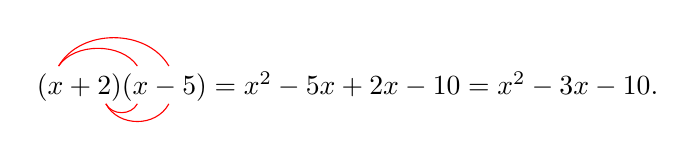
\begin{tikzpicture}
\draw node[right] {$(x+2)(x-5) = x^2-5x+2x-10 = x^2 -3x-10.$};

\pgfmathsetmacro{\klAx}{0.40}
\pgfmathsetmacro{\klBx}{1.00}
\pgfmathsetmacro{\klCx}{1.4}
\pgfmathsetmacro{\klDx}{1.8} 
\pgfmathsetmacro{\klEx}{2.5}
\pgfmathsetmacro{\klLo}{-0.22}
\pgfmathsetmacro{\klHi}{0.26}

\pbezier{\klAx}{\klCx}{\klHi}{0.3}
\pbezier{\klAx}{\klDx}{\klHi}{0.48}

\pbezier{\klBx}{\klCx}{\klLo}{-0.15}
\pbezier{\klBx}{\klDx}{\klLo}{-0.3}
\end{tikzpicture}\newline
\end{esimerkki}

\begin{esimerkki}
Laske binomien $x^2-x$ ja $2x-1$ tulo. \\
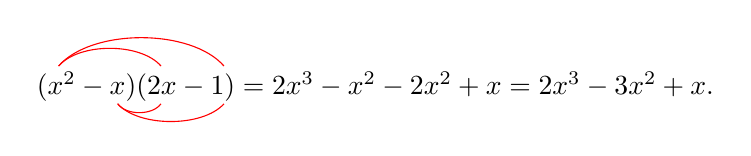
\begin{tikzpicture}
\draw node[right] {$(x^2-x)(2x-1) = 2x^3-x^2-2x^2+x = 2x^3 -3x^2 +x.$};

\pgfmathsetmacro{\klAx}{0.40}
\pgfmathsetmacro{\klBx}{1.15}
\pgfmathsetmacro{\klCx}{1.7}
\pgfmathsetmacro{\klDx}{2.5}
\pgfmathsetmacro{\klEx}{2.7}
\pgfmathsetmacro{\klLo}{-0.22}
\pgfmathsetmacro{\klHi}{0.26}

\pbezier{\klAx}{\klCx}{\klHi}{0.3}
\pbezier{\klAx}{\klDx}{\klHi}{0.48}

\pbezier{\klBx}{\klCx}{\klLo}{-0.15}
\pbezier{\klBx}{\klDx}{\klLo}{-0.3}
\end{tikzpicture}\newline
\end{esimerkki}

Kahden binomin tulon laskusääntö perustellaan soveltamalla osittelulakia kahdesti:


\begin{align*}
(a+b)(c+d) &= (a+b)\cdot c + (a+b)\cdot d &\emph{osittelulaki} \\
 &= ac+bc+ad+bd &\emph{osittelulaki} 
\end{align*}


\subsubsection*{Yleinen kertolasku}

Osittelulain nojalla kahden polynomin tulo saadaan laskemalla yhteen kaikki
termit, jotka saadaan kertomalla termi ensimmäisestä ja toinen termi toisesta
polynomista.


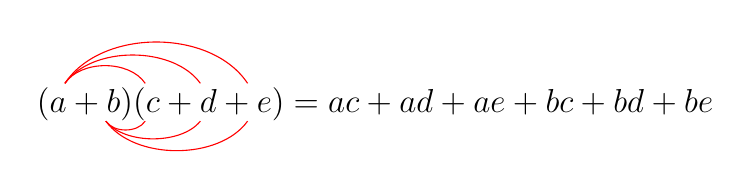
\begin{tikzpicture}
\draw node[right] {\large $(a+b)(c+d+e) = ac+ad+ae+bc+bd+be$};

\pgfmathsetmacro{\klAx}{0.48}
\pgfmathsetmacro{\klBx}{1.0}
\pgfmathsetmacro{\klCx}{1.5}
\pgfmathsetmacro{\klDx}{2.2}
\pgfmathsetmacro{\klEx}{2.8} %oli 3.26
\pgfmathsetmacro{\klLo}{-0.22}
\pgfmathsetmacro{\klHi}{0.26}

\pbezier{\klAx}{\klCx}{\klHi}{0.3}
\pbezier{\klAx}{\klDx}{\klHi}{0.48}
\pbezier{\klAx}{\klEx}{\klHi}{0.7}

\pbezier{\klBx}{\klCx}{\klLo}{-0.15}
\pbezier{\klBx}{\klDx}{\klLo}{-0.3}
\pbezier{\klBx}{\klEx}{\klLo}{-0.5}
\end{tikzpicture}

\begin{esimerkki}
Laske polynomien $x-3$ ja $x^2-4x+3$ tulo. \\
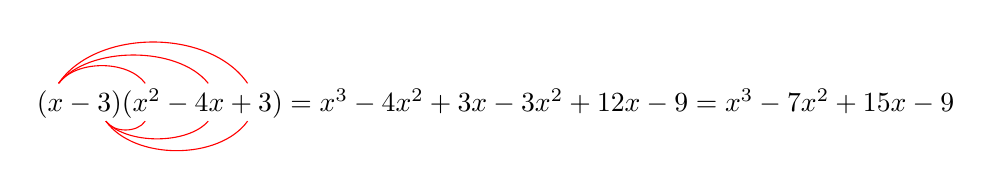
\begin{tikzpicture}
\draw node[right] {$(x-3)(x^2-4x+3) = x^3-4x^2+3x-3x^2+12x-9 = x^3-7x^2+15x-9$};

\pgfmathsetmacro{\klAx}{0.40}
\pgfmathsetmacro{\klBx}{1.00}
\pgfmathsetmacro{\klCx}{1.5}
\pgfmathsetmacro{\klDx}{2.3}
\pgfmathsetmacro{\klEx}{2.8}
\pgfmathsetmacro{\klLo}{-0.22}
\pgfmathsetmacro{\klHi}{0.26}

\pbezier{\klAx}{\klCx}{\klHi}{0.3}
\pbezier{\klAx}{\klDx}{\klHi}{0.48}
\pbezier{\klAx}{\klEx}{\klHi}{0.7}

\pbezier{\klBx}{\klCx}{\klLo}{-0.15}
\pbezier{\klBx}{\klDx}{\klLo}{-0.3}
\pbezier{\klBx}{\klEx}{\klLo}{-0.5}
\end{tikzpicture}\newline
\end{esimerkki}

\begin{esimerkki}
Laske polynomien $x^4-3x^3+3$ ja $x^3-2x^2+1$ tulo. \\
\begin{align*}
&\hspace{0.5cm}(\textcolor{red}{x^4} \textcolor{blue}{-3x^3} +{}\textcolor{blue!30!green}{3})(x^3-2x^2+1) \\
&= \textcolor{red}{x^4}\cdot x^3 + \textcolor{red}{x^4}\cdot (-2x^2)+\textcolor{red}{x^4}\cdot 1\textcolor{blue}{{}-3x^3}\cdot x^3\textcolor{blue}{{}-3x^3}\cdot(-2x^2)\textcolor{blue}{{}-3x^3}\cdot1 \\
&\hspace{0.5cm}+\textcolor{blue!30!green}{3}x^3+\textcolor{blue!30!green}{3}\cdot(-2x^2)+\textcolor{blue!30!green}{3}\cdot 1 \\
&= x^7-2x^6+x^4-3x^6+6x^5-3x^3+3x^3-6x^2+3 \\
&= x^7-5x^6+6x^5+x^4-6x^2+3
\end{align*}
\end{esimerkki}

\subsection*{Muistikaavat}

\qrlinkki{http://opetus.tv/maa/maa2/muistikaavat/}{
Opetus.tv: \emph{muistikaavat} (8:05, 6:38 ja 9:08)}

Joitakin polynomien kertolaskuja tarvitaan niin usein, että niitä kutsutaan \termi{muistikaavat}{muistikaavoiksi}.

\laatikko[Muistikaavat]{
    \begin{tabular}{lrcl}
		& \\        
        {\bf Summan neliö} & $(a+b)^2$ &$=$& $a^2+2ab+b^2$\\
       {\bf Erotuksen neliö} & $(a-b)^2$ &$=$& $a^2-2ab+b^2$ \\
       {\bf Summan ja erotuksen tulo} & $(a+b)(a-b)$ &$=$& $a^2-b^2$ 
    \end{tabular} }

%\laatikko[Muistikaavat]{
%    \begin{description}
%        \item[Summan neliö] $(a+b)^2 = a^2+2ab+b^2$
%        \item[Erotuksen neliö] $(a-b)^2 = a^2-2ab+b^2$
%        \item[Summan ja erotuksen tulo] $(a+b)(a-b) = a^2-b^2$
%    \end{description}
%}

Nämä kaavat voidaan todistaa helposti laskemalla.

\paragraph*{Summan neliö}

\begin{align*}
(a+b)^2 &= (a+b)(a+b) &\emph{neliön määritelmä} \\
% &= a(a+b)+b(a+b) &\emph{osittelulaki} \\
&= a^2+ab+ba+b^2 &\emph{osittelulaki} \\
&= a^2+ab+ab+b^2 &\emph{vaihdannaisuus ($ba=ab$)} \\
&= a^2+2ab+b^2
\end{align*}

\paragraph*{Erotuksen neliö}

\begin{align*}
(a-b)^2 &= (a-b)(a-b) &\emph{neliön määritelmä} \\
% &= a(a-b)-b(a-b) &\emph{osittelulaki} \\
&= a^2-ab-ba+b^2 &\emph{osittelulaki} \\
&= a^2-ab-ab+b^2 &\emph{vaihdannaisuus ($ba=ab$)} \\
&= a^2-2ab+b^2
\end{align*}

Edellä todistettuja kahta muistikaavaa kutsutaan yhdessä nimellä binomin neliö. Toisinaan ne kirjoitetaan yhtenä yhtälönä muodossa $(a \pm b)^2=a^2 \pm 2ab+b^2$. % Kaavoissa useasti esiintyviä $\pm$-merkkejä luetaan siten, että ylemmät ja alemmat täsmäävät keskenään. Ylempien merkkien (kaikki $+$:ia) valinta vastaa siis summan neliötä ja alempien merkkien (kaikki $-$:ia) valinta erotuksen neliötä.

\paragraph*{Summan ja erotuksen tulo}

\begin{align*}
(a+b)(a-b) &= a^2-ab+ba-b^2 &\emph{osittelulaki} \\
&= a^2-ab+ab-b^2 &\emph{vaihdannaisuus ($ba=ab$)} \\
&= a^2-b^2
\end{align*}

\begin{esimerkki}
Sievennä $(x+5)^2$. \\
\quad\\
Käytetään muistikaavaa $(a+b)^2 = a^2+2ab+b^2$. Nyt $a = x$ ja $b = 5$.
Saadaan
        \[ (x+5)^2 = x^2-2\cdot x\cdot 5+5^2 = x^2+10x+25. \]
\end{esimerkki}

\begin{esimerkki}
Sievennä $(3x-2y)^2$. \\
\quad\\
Käytetään muistikaavaa $(a-b)^2 = a^2-2ab+b^2$. Nyt $a = 3x$ ja $b = 2y$.
Saadaan
        \[ (3x+2y)^2 = (3x)^2-2\cdot 3x\cdot 2y+(2y)^2 = 9x^2-12xy+4y^2. \]
\end{esimerkki}

\begin{esimerkki}
Laske ilman laskinta a) $995^2$ b) $104 \cdot 96$. \\
Käytetään ovelasti muistikaavoja $(a-b)^2 = a^2-2ab+b^2$ ja \mbox{$(a+b)(a-b) = a^2-b^2$}.
\begin{alakohdat}
\alakohta{$995^2 = (1000-5)^2 = 1000^2-2\cdot 1000\cdot 5+5^2 = 1000000-10000+25 = 990025 $}
\alakohta{$104\cdot 96 = (100+4)(100-4) = 100^2 - 4^2 = 10000 - 16 = 9984$.}
\end{alakohdat}
\end{esimerkki}

\begin{tehtavasivu}

\paragraph*{Opi perusteet}

\begin{tehtava}
    Sievennä.
    \begin{alakohdat}
        \alakohta{$x\cdot x^2$}
        \alakohta{$5x\cdot 3x$}
        \alakohta{$-2(-5x^3)$}
        \alakohta{$3x^2\cdot(-6x^4)$}
    \end{alakohdat}
    \begin{vastaus}
        \begin{alakohdat}
            \alakohta{$x^3$}
            \alakohta{$15x^2$}
            \alakohta{$10x^3$}
            \alakohta{$-18x^6$}
        \end{alakohdat}
    \end{vastaus}
\end{tehtava}

\begin{tehtava}
    Sievennä.
    \begin{alakohdat}
        \alakohta{$2(x+3)$}
        \alakohta{$x(x - 2)$}
        \alakohta{$3x(1-2x)$}
        \alakohta{$x^2(x + 5)$}
    \end{alakohdat}
    \begin{vastaus}
        \begin{alakohdat}
            \alakohta{$2x+6$}
            \alakohta{$x^2 - 2x$}
            \alakohta{$3x-6x^2$}
            \alakohta{$x^3 + 5x^2$}
        \end{alakohdat}
    \end{vastaus}
\end{tehtava}

\begin{tehtava}
    Sievennä.
    \begin{alakohdat}
        \alakohta{$3(x+2y-4)$}
        \alakohta{$(x+2)(x + 3)$}
        \alakohta{$(3-x)(2x-1)$}
\end{alakohdat}
    \begin{vastaus}
        \begin{alakohdat}
            \alakohta{$3x+6y-12$}
            \alakohta{$x^2 +5x+6$}
            \alakohta{$-2x^2+7x-3$}
        \end{alakohdat}
    \end{vastaus}
\end{tehtava}

\begin{tehtava}
    Kerro sulut auki muistikaavan avulla.
    \begin{alakohdat}
        \alakohta{$(x+y)^2$}
        \alakohta{$(x-y)^2$}
        \alakohta{$(x+y)(x-y)$}
    \end{alakohdat}
    \begin{vastaus}
        \begin{alakohdat}
        \alakohta{$x^2 +2xy+y^2$}
        \alakohta{$x^2 -2xy +y^2$}
        \alakohta{$x^2-y^2$}
        \end{alakohdat}
    \end{vastaus}
\end{tehtava}

\begin{tehtava}
    Kerro sulut auki muistikaavan avulla.
    \begin{alakohdat}
        \alakohta{$(x+3)^2$}
        \alakohta{$(y-5)^2$}
        \alakohta{$(x-4)(x+4)$}
        \alakohta{$(3x+2)^2$}
    \end{alakohdat}
    \begin{vastaus}
        \begin{alakohdat}
        \alakohta{$x^2 +6x+9$}
        \alakohta{$y^2 - 10y+25$}
        \alakohta{$x^2 -16$}
        \alakohta{$9x^2 +12x +4$}
        \end{alakohdat}
    \end{vastaus}
\end{tehtava}



\begin{tehtava}
%Siirretty MAA1-kirjan juuret-kappaleesta
%Tehtävän laatinut Johanna Rämö 9.11.2013.
%Ratkaisun tehnyt Johanna Rämö 9.11.2013.
Osoita, että seuraavat laskukaavat eivät päde. Tee se etsimällä konkereettiset reaaliluvut $a$ ja $b$, joilla yhtälö ei päde.
        \begin{alakohdat}
        \alakohta{$(a+b)^2=a^2+b^2$}
        \alakohta{$\sqrt{a+b}=\sqrt{a}+\sqrt{b}$}
        \alakohta{$\dfrac{3a}{3b+c}=\dfrac{a}{b+c}$}
        \end{alakohdat}
        
        \begin{vastaus}
        \begin{alakohdatrivi}
            \alakohta{Kaava ei päde, sillä esimerkiksi $(1+2)^2=3^2=9$, mutta $1^2+2^2=1+4=5$.}
            \alakohta{Kaava ei päde, sillä esimerkiksi $\sqrt{1+1}=\sqrt{2}$, mutta $\sqrt{1}+\sqrt{1}=1+1=2$.}
            \alakohta{Kaava ei päde, sillä esimerkiksi
            $$\frac{3 \cdot 2}{3 \cdot 1+1}=\frac{6}{5}$$,
            mutta $$\frac{2}{1+1}=1$$.}
        \end{alakohdatrivi}
        \end{vastaus}
\end{tehtava}

%\begin{tehtava}
%    Sievennä lauseke $(x^2+1)(x^3-2x)$. Mikä on polynomin aste?
%    \begin{vastaus}
%        Lauseke sievenee muotoon $x^5-x^3-2x$. Polynomin aste on $5$.
%    \end{vastaus}
%\end{tehtava}

\paragraph*{Hallitse kokonaisuus}

\begin{tehtava}
    Pohdi ja määritä sulkuja avaamatta lausekkeen $(x^2+1)(x^3-2x)$
    \begin{alakohdat}
        \alakohta{aste}
        \alakohta{vakiotermi.}
    \end{alakohdat}
    \begin{vastaus}
        \begin{alakohdat}
            \alakohta{Polynomin aste on kunkin tekijän korkeimpien asteiden summa, tässä siis $2+3=5$.}
            \alakohta{Polynomin vakiotermi on kunkin tekijän vakiotermien tulo, tässä siis $1\cdot 0=0$.}
        \end{alakohdat}
    \end{vastaus}
\end{tehtava}

\begin{tehtava}
    Sievennä.
    \begin{alakohdat}
        \alakohta{$(-2x)(4x - 1)\cdot 3$}
        \alakohta{$(-x^3)(10x - 2)$}
        \alakohta{$5(-2x + 1)(-9x) $}
        \alakohta{$2x(x-3)+1$}
    \end{alakohdat}
    \begin{vastaus}
        \begin{alakohdat}
            \alakohta{$-24x^2 + 6x$}
            \alakohta{$-10x^4 + 2x^3$}
            \alakohta{$90x^2 - 45x$}
            \alakohta{$2x^2-6x+1$}
        \end{alakohdat}
    \end{vastaus}
\end{tehtava}

\begin{tehtava}
    Sievennä muistikaavojen avulla.
    \begin{alakohdat}
        \alakohta{$(x+6)^2$}
        \alakohta{$(3y-1)^2$}
        \alakohta{$(-3-x)(x-3) $}

    \end{alakohdat}
    \begin{vastaus}
        \begin{alakohdat}
            \alakohta{$x^2 + 12x + 36$}
            \alakohta{$9y^2 - 6y + 1$}
            \alakohta{$9-x^2$}
        \end{alakohdat}
    \end{vastaus}
\end{tehtava}

\begin{tehtava}
    Sievennä muistikaavojen avulla.
    \begin{alakohdat}
        \alakohta{$(5-x)^2$}
        \alakohta{$(7x + 4)^2$}
        \alakohta{$(9 - 7x)(9 + 7x)$}
        \alakohta{$(8x - 8)(8x + 8)$}
    \end{alakohdat}
    \begin{vastaus}
        \begin{alakohdat}
            \alakohta{$x^2 - 10x + 25$}
            \alakohta{$49x^2 + 56x + 16$}
            \alakohta{$-49x^2 + 81$}
            \alakohta{$64x^2 - 64$}
        \end{alakohdat}
    \end{vastaus}
\end{tehtava}

\begin{tehtava}
    Sievennä.
    \begin{alakohdat}
        \alakohta{$(2y+5)(y+7)$}
        \alakohta{$(x-1)(x+4)x$}
    \end{alakohdat}
    \begin{vastaus}
        \begin{alakohdat}
            \alakohta{$2y^2 + 19y + 35$}
            \alakohta{$x^3 + 3x^2 - 4x$}
        \end{alakohdat}
    \end{vastaus}
\end{tehtava}

\begin{tehtava}
    Osoita, että
    \begin{alakohdat}
        \alakohta{$(t+v)^2+(t-v)^2=2t^2+2v^2$}
        \alakohta{$(t+v)^2-(t-v)^2 = 4tv$.}
    \end{alakohdat}
    \begin{vastaus}
    	Sievennetään yhtälöiden vasempia puolia:
        \begin{alakohdat}
            \alakohta{$(t+v)^2+(t-v)^2 = t^2+2tv+v^2+t^2-2tv+v^2 = 2t^2+2v^2$.}
            \alakohta{$(t+v)^2-(t-v)^2 = t^2+2tv+v^2-t^2+2tv-v^2 = 4tv$.}
        \end{alakohdat}
    \end{vastaus}
\end{tehtava}

\begin{tehtava}
    Esitä tulona, eli käytä muistikaavaa toiseen suuntaan.
    \begin{alakohdat}
        \alakohta{$a^2+2ab+b^2$}
        \alakohta{$x^2+2x+1$}
        \alakohta{$y^2-4y+4$}
        \alakohta{$a^2-25$}
    \end{alakohdat}
    \begin{vastaus}
        \begin{alakohdat}
            \alakohta{$(a+b)^2$}
            \alakohta{$(x+1)^2$}
            \alakohta{$(y-2)^2$}
            \alakohta{$(a+5)(a-5)$}
        \end{alakohdat}
    \end{vastaus}
\end{tehtava}


\begin{tehtava}
	Tiedetään, että $(a+b)^2=12$ ja $(a-b)^2=4$. Ratkaise tulon $ab$ suuruus.
    \begin{vastaus}
	$ab = 2$. Käytä muistikaavoja.
    \end{vastaus}
\end{tehtava}


\begin{tehtava}
(YO 1888 1) Mikä on a/b:n arvo, jos \\
$ (\sqrt{a}+\sqrt{b}):(\sqrt{a}-\sqrt{b})=\sqrt{2}$ ?
\begin{vastaus}
$(3-2\sqrt{2}):(3+2\sqrt{2})$
\end{vastaus}
\end{tehtava}


\begin{tehtava}
Ensimmäisen asteen polynomiausekkeen yleinen muoto on $ax+b$, missä $x$ on muuttuja, ja $a$ ja $b$ ovat (reaalisia) vakioita. Osoita, että jos $P$ ja $Q$ ovat ensimmäisen asteen polynomifunktioita, niin tällöin $P(Q(x)$ ja $Q(P(x))$ ovat myös ensimmäistä astetta.


\begin{vastaus}

Voidaan merkitään $P(x)=ax+b$ ja $Q(x)=cx+d$, koska molemmat funktiot ovat ensimmäisen asteen polynomifunktioita. (Käytämme kertoimien merkitsemiseen eri kirjaimia, sillä lausekkeiden vakiot saattavat olla keskenään erisuuret.) Sievennetään $P(Q(x))$: $P(Q(x))=P(cx+d)=a(cx+d)+b=acx+ad+b$. Todetaan, että jos $a$ ja $c$ ovat reaalilukuvakioita, niin myös niiden tulo on reaalilukuvakio. Sama pätee vakioille $a$ ja $d$, joiden tulo ja myös kyseisen tulon ja $b$:n summa on vakio. Merkitään havainnollistamisen vuoksi $ac=e$, ja $ad+b=f$. Nyt lauseke $acx+ad+b$ voidaan kirjoittaa uudelleen muodossa $ex+f$, josta nähdään selvästi kyseessä olevan ensimmäisen asteen polynomi.

Väite osoitetaan järjestykselle $Q(P(x)$ samalla tavalla, minkä jälkeen väite on todistettu.

\end{vastaus}
\end{tehtava}


\paragraph*{Lisää tehtäviä}

\begin{tehtava}
   	Muistikaavat on opittava ulkoa ja niiden käytön tulee automatisoitua.
	Laske siis nämä käyttäen muistikaavoja. Tavoite on kirjoittaa vastaus suoraan ilman välivaiheita. Jos se ei vielä onnistu, yritä selvitä yhdellä välivaiheella.
    \begin{alakohdat}
        \alakohta{$(x+2)^2$}
        \alakohta{$(x-5)^2$}
        \alakohta{$(b+4)(b-4)$}
        \alakohta{$(x-1)^2$}
            \alakohta{$(2x+1)^2$}
            \alakohta{$(1-a)(1+a)$}
            \alakohta{$(x-7)^2$}
            \alakohta{$(y+1)^2$}
            \alakohta{$(x-3y)^2$}
            \alakohta{$(3x-1)^2$}
            \alakohta{$(2x+1)(2x-1)$}
            \alakohta{$(t-2)^2$}
            \alakohta{$(2x+3)^2$}
            \alakohta{$(2-a)^2$}
            \alakohta{$(5x+2)(5x-2)$}
            \alakohta{$(3-c)(3+c)$}
            \alakohta{$(10x-1)^2$}
            \alakohta{$(2a+b)^2$}            
            \alakohta{$(x+6)^2$}                                                                                                                                                        
    \end{alakohdat}
    \begin{vastaus}
        \begin{alakohdat}
            \alakohta{$x^2+4x+4$}
            \alakohta{$x^2-10x+25$}
            \alakohta{$b^2-16$}
            \alakohta{$x^2-2x+1$}
            \alakohta{$4x^2+4x+1$}
            \alakohta{$1-a^2$}
            \alakohta{$x^2-14x+49$}
            \alakohta{$y^2+2y+1$}
            \alakohta{$x^2+6xy+9y^2$}
            \alakohta{$9x^2-6x+1$}
            \alakohta{$4x^2-1$}
            \alakohta{$t^2-4t+4$}
            \alakohta{$4x^2+12x+9$}
            \alakohta{$a^2-4a+4$}
            \alakohta{$25x^2-4$}
            \alakohta{$9-c^2$}                                                                                                                                    
            \alakohta{$100x^2-20x+1$}            
            \alakohta{$4a^2+4ab+b^2$}                                                                                                                                                        
            \alakohta{$x^2+12x+36$}                                                                                                                                                        
        \end{alakohdat}
    \end{vastaus}
\end{tehtava}


\begin{tehtava}
   	Muistikaavan mukaisen lausekkeen tunnistaminen on tärkeää.
Tunnista edellisessä tehtävässä laskemasi muistikaavat ja
   	esitä lausekkeet alkuperäisessä muodossaan tulona.
    \begin{alakohdat}
            \alakohta{$1-a^2$} 
	        \alakohta{$a^2-4a+4$}
            \alakohta{$4x^2+4x+1$}
            \alakohta{$x^2-14x+49$}
            \alakohta{$100x^2-20x+1$}            
            \alakohta{$4a^2+4ab+b^2$}                                                                                                                                                        
            \alakohta{$y^2+2y+1$}
            \alakohta{$x^2+4x+4$}
            \alakohta{$4x^2-1$}
            \alakohta{$t^2-4t+4$}
            \alakohta{$25x^2-4$}
            \alakohta{$b^2-16$}
            \alakohta{$x^2-2x+1$}
            \alakohta{$9-c^2$}                                                                                                                                    
            \alakohta{$x^2+12x+36$}                                                                                                                                                        
            \alakohta{$4x^2+12x+9$}            
            \alakohta{$x^2-10x+25$}
            \alakohta{$x^2+6xy+9y^2$}
            \alakohta{$9x^2-6x+1$}
    \end{alakohdat}
    \begin{vastaus}
        \begin{alakohdat}
            \alakohta{$(1-a)(1+a)$} 
            \alakohta{$(a-2)^2$}
            \alakohta{$(2x+1)^2$}
            \alakohta{$(x-7)^2$}
            \alakohta{$(10x-1)^2$}
            \alakohta{$(2a+b)^2$}   
            \alakohta{$(y+1)^2$}
   		     \alakohta{$(x+2)^2$}
            \alakohta{$(2x+1)(2x-1)$}
             \alakohta{$(t-2)^2$}
            \alakohta{$(5x+2)(5x-2)$}
    	    \alakohta{$(b+4)(b-4)$}
 	       \alakohta{$(x-1)^2$}
            \alakohta{$(3-c)(3+c)$}
            \alakohta{$(x+6)^2$}                                                                                                                                                         
            \alakohta{$(2x+3)^2$}            
  		    \alakohta{$(x-5)^2$}  
            \alakohta{$(x-3y)^2$}
            \alakohta{$(3x-1)^2$}
         \end{alakohdat}
    \end{vastaus}
\end{tehtava}

\begin{tehtava}
    Esitä tulona, eli käytä muistikaavaa toiseen suuntaan.
    \begin{alakohdat}
        \alakohta{$4b^2-4b+1$}
        \alakohta{$16t^2-9$}
        \alakohta{$9x^2+12xy+4y^2$}
        \alakohta{$x^2-x+\frac{1}{4}$}
        \alakohta{$x^2-2$}
    \end{alakohdat}
    \begin{vastaus}
        \begin{alakohdat}
            \alakohta{$(2b-1)^2$}
            \alakohta{$(4t+3)(4t-3)$}
            \alakohta{$(3x+2y)^2$}
            \alakohta{$(x-\frac{1}{2})^2$}
            \alakohta{$(x-\sqrt{2})(x+\sqrt{2})$}
        \end{alakohdat}
    \end{vastaus}
\end{tehtava}

\begin{tehtava}
	Sievennä. 
	\begin{alakohdat}
		\alakohta{$(x-3)(2x^3-3x+4)$}
		\alakohta{$(x^2+1)(x^3-2x-4)$}
		\alakohta{$(x-1)(x^4+x^3+x^2+x+1)$}
		\alakohta{$(\frac x5-\frac23)(x^2+x+1)$}
	\end{alakohdat}
	\begin{vastaus}
		\begin{alakohdat}
			\alakohta{$2x^4-6x^3-3x^2+13x-12$}
			\alakohta{$x^5-x^3-4x^2-2x-4$}
			\alakohta{$x^5-1$}
			\alakohta{$\frac15x^3-\frac{7}{15}x^2-\frac{7}{15}x-\frac23$}
		\end{alakohdat}
	\end{vastaus}
\end{tehtava}

\begin{tehtava}
    Sievennä.
    \begin{alakohdat}
            \alakohta{$(a+b)^3$}
            \alakohta{$(a+b)^4$}
            \alakohta{$(a-b)^3$}
        \end{alakohdat}
    \begin{vastaus}
        \begin{alakohdat}
            \alakohta{$(a+b)^3 = a^3 + 3a^2b + 3ab^2 + b^3$}
            \alakohta{$(a+b)^4 = a^4 + 4a^3b + 6a^2b^2 + 4ab^3 + b^4$}
            \alakohta{$(a-b)^3 = a^3 - 3a^2b + 3ab^2 - b^3$}
        \end{alakohdat}
    \end{vastaus}
\end{tehtava}

\begin{tehtava}
    Laske ovelasti muistikaavojen avulla:
    \begin{alakohdat}
        \alakohta{$101^2=(100+1)^2= \ldots$}
        \alakohta{$99^2$}
        \alakohta{$49\cdot 51$}
        \alakohta{$35^2-25^2$}
        \alakohta{$170^2-30^2$}
    \end{alakohdat}
    \begin{vastaus}
        \begin{alakohdat}
            \alakohta{$(100+1)^2=100^2+2\cdot 100 \cdot 1 + 1^2=10201$}
            \alakohta{$99^2=(100-1)^2=100^2-2\cdot 100 \cdot 1 + 1^2=9801 $}
            \alakohta{$49\cdot 51=(50-1)(50+1)=50^2-1^2=2500-1=2499$}
            \alakohta{$35^2-25^2 = (35+25)(35-25)=60 \cdot 10 = 600$}
            \alakohta{$170^2-30^2 = (170+30) \cdot (170-30)^2 = 200 \cdot 140 = 28000$}
        \end{alakohdat}
    \end{vastaus}
\end{tehtava}

%\begin{tehtava}
%    Sievennä. (Ohje: käytä summakaavoja.)
%    \begin{alakohdat}
%        \alakohta{$63^2+37^2$}
%        \alakohta{$101^2+99^2$}
%    \end{alakohdat}
%    \begin{vastaus}
%        \begin{alakohdat}
%            \alakohta{$63^2+37^2 = (50+13)^2+(50-13)^2 = 2\cdot 50^2 + 2\cdot 13^2 = 2\cdot 2500 +2\cdot 169 = 5000 + 338 = 5338$}
%            \alakohta{$101^2+99^2 = (100+1)^2+(100-1)^2 = 2\cdot 100^2 + 2\cdot 1^2 = 2\cdot 10000 + 2\cdot 1 = 20000 + 2 = 20002$}
%        \end{alakohdat}
%    \end{vastaus}
%\end{tehtava}

\begin{tehtava}
    Olkoon $P(x)=-x^4+2x$ reaalifunktio. Sievennä lausekkeet.
    \begin{alakohdat}
		\alakohta{$P(\sqrt{2})$}
        \alakohta{$P(x)^2$}
        \alakohta{$P(-x)$}
        \alakohta{$P(2t)$}
    \end{alakohdat}
    \begin{vastaus}
        \begin{alakohdat}
            \alakohta{$-4 + 2\sqrt{2}$}
            \alakohta{$x^8 - 4x^5 + 4x^2$}
            \alakohta{$-x^4-2x$}
            \alakohta{$-16t^4+4t$}
        \end{alakohdat}
    \end{vastaus}
\end{tehtava}

\begin{tehtava}
    Olkoot $P(x)=x^2$ ja $Q(x)=x+1$ reaalifunktioita. Sievennä lausekkeet.
    \begin{alakohdat}
        \alakohta{$P(x+1)$}
        \alakohta{$Q(x-1)$}
        \alakohta{$P(Q(x))$}
        \alakohta{$Q(P(x))$}
    \end{alakohdat}
    \begin{vastaus}
        \begin{alakohdat}
            \alakohta{$P(x+1) = (x+1)^2 = x^2+2x+1$}
            \alakohta{$Q(x-1) = (x-1)+1 = x$}
            \alakohta{$P(Q(x)) = P(x+1) = (x+1)^2 = x^2+2x+1$}
            \alakohta{$Q(P(x)) = Q(x^2) = x^2+1$}
        \end{alakohdat}
    \end{vastaus}
\end{tehtava}

\begin{tehtava} 
	Yllättäviä yhteyksiä:
    \begin{alakohdat}
            \alakohta{Perustele, että $\left(2+\sqrt{3}\right)^{-1}= 2-\sqrt{3}$.} 
            \alakohta{Perustele, että $\left(4+\sqrt{3}\right)^{-1} \neq 4-\sqrt{3}$.} 
	        \alakohta{$\star$ Etsi lisää a-kohdan kaltaisia lukuja. Mikä on niiden
	        yleinen muoto?}
    \end{alakohdat}

    \begin{vastaus}
    \begin{alakohdat}
            \alakohta{Tutki lukujen $2+\sqrt{3}$ ja $2-\sqrt{3}$ tuloa.} 
            \alakohta{Lukujen $4+\sqrt{3}$ ja $4-\sqrt{3}$ tulo on 13, joten ne
            eivät ole käänteislukuja.} 
	        \alakohta{Yleisesti $\left(a+\sqrt{a^2-1}\right)^{-1}= a-\sqrt{a^2-1}$}
    \end{alakohdat}
    \end{vastaus}
\end{tehtava}

\begin{tehtava} %Vaikea!
    $\star$ Kahden luvun keskiarvo on $7$. Kuinka suuri niiden tulo voi korkeintaan olla? Perustele.
    \\ (Keksit vastauksen todennäköisesti helpommin kuin sen perustelun.)
    \begin{vastaus}
        $49$. Perustelu muistikaavoilla: Jos lukujen keskiarvo on $7$, ne ovat muotoa $7+a$ ja $7-a$. Lasketaan tulo: $(7+a)(7-a)=7^2-a^2 = 49-a^2 \geq 49$. Siis 49 on suurin
        mahdollinen.
    \end{vastaus}
\end{tehtava}

\end{tehtavasivu}
	%polynomin kertominen monomilla a(x+b)=ax+ab
	%kahden binomin tulo: (a+b)(c+d)=ac+ad+bc+bd
	%tekijöihin jako, käsite tekijä
	%muistikaavat
		%(a+b)^2=a^2+2ab+b^2
		%(a-b)^2=a^2-2ab+b^2
		%(a-b)(a+b)=a^2-b^2
		%Esimerkki tai harjoitustehtävä: 102*98=(100+2)(100-2)=10000-4

	\section{Tulon nollasääntö ja tulon merkkisääntö}

\subsection*{Tulon merkkisääntö}

Pitkän matematiikan 1. kurssilla on esitetty seuraava sääntö kahden luvun tulolle:

\laatikko[Tulon merkkisääntö kahdelle tulon tekijälle]{
    \begin{itemize}
        \item Jos tulon tekijät ovat samanmerkkisiä, tulo on positiivinen.
        \begin{itemize}
	        \item Kahden positiivisen luvun tulo on positiivinen.
	        \item Kahden negatiivisen luvun tulo on positiivinen.
        \end{itemize}
        \item Jos tulon tekijät ovat erimerkkisiä, tulo on negatiivinen.
        \begin{itemize}
	        \item Positiivisen ja negatiivisen luvun tulo on negatiivinen.
        \end{itemize}
    \end{itemize}
}

Tulon merkkisäännöstä seuraa, että luvun neliö ei voi olla negatiivinen. (Koska kahden samanmerkkisen luvun tulo on positiivinen.) Lyhyemmin ilmaistuna $x^2 \geq 0$.

\begin{esimerkki}
Osoita, että funktio $P(x)=x^2+7$ saa vain positiivisia arvoja.
    \begin{esimratk}
	Koska $x^2 \geq 0$, lausekkeen $x^2+7$ arvo on vähintään $7$. Fuktio saa siis
	vain positiivisia arvoja.
    \end{esimratk}
\end{esimerkki}

\begin{esimerkki}
Mikä on funktion $f:\mathbb{R} \rightarrow \mathbb{R}, f(t)=-t^4+3$ suurin arvo?
    \begin{esimratk}
	Koska muuttuja $t$ on reaaliluku, ei sen parillinen potenssi voi olla negatiivinen, vaan $t^4$:n arvo on vähintään $0$. Tämän perusteella $-t^4$:n arvo on epäpositiivinen eli korkeintaan nolla. Jos $-t^4$:n suurin arvo on nolla, niin lisäämällä tähän luvun $3$, saadan funktion $f(t)=-t^4+3$ suurimmaksi arvoksi $3$.
    \end{esimratk}
\end{esimerkki}

%\begin{esimerkki}
%Määritä polynomin $x^2+2x+2$ suurin/pienin arvo.
%    \begin{esimratk}
%	Polynomissa on kolme termiä, ja näiden vaikutusta polynomin arvoon on hankala tarkastella yhdessä. Muokataan polynomia ...
%    \end{esimratk}
%\end{esimerkki}

Tulon merkkisääntö yleistyy mille tahansa määrälle tulontekijöitä.
Mikäli tulossa on pariton $(1, 3, 5, \ldots)$ määrä negatiivisia tekijöitä, tulo on negatiivinen.
Muulloin tulo on positiivinen.

%Hyödynnämme merkkisääntöä myöhemmin, kun teemme epäyhtälöistä merkkikaavioita.

\newpage

\subsection*{Tulon nollasääntö}

Tulon merkkisäännöstä seuraa, että positiivisten ja negatiivisten lukujen tulo on aina positiivinen tai negatiivinen, ei koskaan nolla.
Jos siis tulo on $0$, tulon tekijöistä ainakin yhden täytyy olla $0$.
Toisaalta jos jokin tulon tekijöistä on $0$, myös tulo on automaattisesti $0$.
Nämä tiedot yhdistämällä saadaan tulon nollasääntö:

\laatikko[Tulon nollasääntö]{
	\begin{description}
		\item Jos jokin tulon tekijöistä on $0$, tulo on $0$.
		\item Jos tulo on $0$, ainakin yksi tulon tekijöistä on $0$.
	\end{description}
}

%TODO: tästä voisi minusta varsin hyvin jättää pois tuon ensimmäisen kohdan T: Jokke
% Jep, niin voisi tehdä ongelmitta. Pitäisin kuitenkin tässä, koska liittyvät toisiinsa. -Ville

\begin{esimerkki}
Sievennä lauseke $(x^5-7)\cdot y \cdot 0\cdot(3a-5b)^2$.
    \begin{esimratk}
	Koska tulossa on tekijänä $0$, vastaus on $0$.
    \end{esimratk}
\end{esimerkki}

\begin{esimerkki} Ratkaistaan yhtälö $(x+5) \cdot x =0 $.
    \begin{align*}
        (x+5)\cdot x &=0 \quad \ppalkki \text{ tulon nollasääntö} \\
        x +5= 0 \text{ tai } x &=0 \\
        x= -5 \text{ tai } x &=0.
    \end{align*}
    Ratkaisuja on siis kaksi, $x= -5$ tai $x= 0$.
\end{esimerkki}

%\begin{esimerkki}
%	\[2(x+5)=0\]
%	Nyt tulon nollasäännön perusteella tiedetään, että $2=0$ tai $x+5=0$.
%	Koska selvästi $2\neq 0$, jää ainoaksi ratkaisuksi $x+5=0$ eli $x=-5$.
%\end{esimerkki}

% \begin{esimerkki} Ratkaistaan $y$ yhtälöstä
%     \[(x^5+5x+5)\cdot 0\cdot \sqrt{x^3-1} =y\]
%     Koska vasemmalla puolella yksi tulon tekijöistä on $0$, tiedämme, että tulo on $0$. Siis $y=0$.
% \end{esimerkki}

%TODO: onko alla oleva järkevä? mistä tietää, mitä muuttujia on tarkoitus ratkaista. minusta vain sekoittaa asioita T: Jokke
\begin{esimerkki} Ratkaise yhtälö
    \[xyz=0.\]
Tulon nollasäännön perusteella $x=0$, $y=0$ tai $z=0$. Nollia voi siis
olla 1--3 kappaletta.
\end{esimerkki}

\begin{tehtavasivu}

\paragraph*{Opi perusteet}

\begin{tehtava}
	Laske.
	\begin{alakohdat}
		\alakohta{$2 \cdot 3$}
		\alakohta{$2 \cdot (-3)$}
		\alakohta{$-2 \cdot 3$}
		\alakohta{$-2 \cdot (-3)$}
		\alakohta{$17 \cdot 666 \cdot 0 \cdot (-31)$}
	\end{alakohdat}
	
	\begin{vastaus}
		\begin{alakohdat}
			\alakohta{$6$}
			\alakohta{$-6$}
			\alakohta{$-6$}
			\alakohta{$6$}
			\alakohta{$0$}
		\end{alakohdat}
	\end{vastaus}
\end{tehtava}

\begin{tehtava}
	Olkoon $a>0$, $b<0$, ja $c=0$. Mitä voit päätellä tulon merkistä?
	\begin{alakohdat}
		\alakohta{$a \cdot a$}
		\alakohta{$b \cdot a$}
		\alakohta{$b \cdot b$}
		\alakohta{$b \cdot c$}
	\end{alakohdat}
	
	\begin{vastaus}
		\begin{alakohdat}
			\alakohta{tulo $>0$}
			\alakohta{tulo $<0$}
			\alakohta{tulo $>0$}
			\alakohta{tulo on $0$}
		\end{alakohdat}
	\end{vastaus}
\end{tehtava}


\begin{tehtava}
    Ratkaise seuraavat yhtälöt käyttämällä tulon nollasääntöä.
    \begin{alakohdat}
        \alakohta{$x(3+x)=0$}
        \alakohta{$(x-4)(x+3)=0$}
		\alakohta{$0=x^2(x-5)$}
    \end{alakohdat}
    \begin{vastaus}
        \begin{alakohdat}
            \alakohta{$x=0$ tai $x=-3$}
            \alakohta{$x=4$ tai $x=-3$}
            \alakohta{$x=0$ tai $x=5$}
        \end{alakohdat}
    \end{vastaus}
\end{tehtava}

\paragraph*{Hallitse kokonaisuus}

\begin{tehtava}
	Olkoon $a > 0$. Mitkä vaihtoehdoista $b>0$, $b<0$, $b=0$ ovat mahdollisia, jos
	tiedetään, että
	\begin{alakohdat}
		\alakohta{$a \cdot b > 0$}
		\alakohta{$a \cdot b \leq 0$}
		\alakohta{$b \cdot b > 0$}
		\alakohta{$b \cdot b < 0$?}
	\end{alakohdat}
	\begin{vastaus}
		\begin{alakohdat}
			\alakohta{$b>0$}
			\alakohta{$b < 0$ ja $b = 0$}
			\alakohta{$b>0$ ja $b<0$}
			\alakohta{Mikään vaihtoehto ei kelpaa.}
		\end{alakohdat}
	\end{vastaus}
\end{tehtava}

\begin{tehtava}
    Ratkaise seuraavat yhtälöt käyttämällä tulon nollasääntöä.
    \begin{alakohdat}
        \alakohta{$y(y+4)=0$}
        \alakohta{$(x-2)(x-1)(x+5)=0$}
        \alakohta{$(x+1)(x^2+2)=0$}
    \end{alakohdat}
    \begin{vastaus}
        \begin{alakohdat}
            \alakohta{$y=0$ tai $y=-4$}
            \alakohta{$x=2$, $x=1$ tai $x=-5$}
            \alakohta{$x=-1$}
        \end{alakohdat}
    \end{vastaus}
\end{tehtava}

\begin{tehtava} 
Osoita, että funktio $f(x)=x^4+3x^2+1$ saa vain positiivisia arvoja.
    \begin{vastaus}
     $x^4\geq 0$ ja $x^2 \geq 0$, joten $f(x) \geq 1$.
    \end{vastaus}
\end{tehtava}

\paragraph*{Lisää tehtäviä}

\begin{tehtava}
	Olkoon $a \geq 0$, $b \leq 0$, ja $c=0$. Mitä voit päätellä tulon merkistä?
	\begin{alakohdat}
		\alakohta{$a \cdot a$}
		\alakohta{$b \cdot a$}
		\alakohta{$b \cdot c$}
	\end{alakohdat}
	
	\begin{vastaus}
		\begin{alakohdat}
			\alakohta{tulo $\geq 0$}
			\alakohta{tulo $\leq 0$}
			\alakohta{tulo on $0$}
		\end{alakohdat}
	\end{vastaus}
\end{tehtava}

\begin{tehtava}
    Ratkaise seuraavat yhtälöt käyttämällä tulon nollasääntöä.
    \begin{alakohdat}
        \alakohta{$(\smiley{}+1)\cdot (t+1)=0$}
        \alakohta{$x(x-5)=0$}
        \alakohta{$(2w+2)^2=0$}
    \end{alakohdat}
    \begin{vastaus}
        \begin{alakohdat}
            \alakohta{$\smiley{}=-1$ tai $t=-1$,\qquad  Symboli $\smiley{}$ esittää jotain lukua, sillä muutoin laskutoimitukset eivät olisi mielekkäitä. Tehtävässä ei myöskään ole selvää, minkä muuttujan suhteen yhtälö pitäisi ratkaista. Siksi on ratkaistu molempien muuttujien suhteen.}
            \alakohta{$x=0$ tai $x=5$}
            \alakohta{$w=-1$}
        \end{alakohdat}
    \end{vastaus}
\end{tehtava}

\begin{tehtava}
    Sievennä seuraava lauseke: $(a-x)\cdot(b-x)\cdot(c-x)\cdot...\cdot(\mathring{a}-x)\cdot(\ddot{a}-x)\cdot(\ddot{o}-x)$.
    \begin{vastaus}
        Tulossa esiintyy tekijänä $(x-x)=0$. Niinpä tulon nollasäännön mukaan
        \begin{align*}
            &(a-x)\cdot(b-x)\cdot(c-x)\cdot...\cdot(x-x)\cdot...\cdot(\ddot{a}-x)\cdot(\ddot{o}-x) \\
            =&(a-x)\cdot(b-x)\cdot(c-x)\cdot...\cdot 0\cdot...\cdot(\ddot{a}-x)\cdot(\ddot{o}-x) \\
            =&0
        \end{align*}
    \end{vastaus}
\end{tehtava}



\begin{tehtava} %
$\star$ Osoita, että $x^2+\frac{1}{x^2}\geq 2$, kun $x \neq 0$.
    \begin{vastaus}
     Aloita tiedosta $\left(x-\frac{1}{x}\right)^2 \geq 0$ ja sievennä.
    \end{vastaus}
\end{tehtava}

\begin{tehtava} 
$\star$ Osoita, että kun $a \geq 0$ ja $b \geq 0$, pätee \\ $\frac{a+b}{2} \geq \sqrt{ab}$. Milloin yhtäsuuruus on voimassa?
    \begin{vastaus}
     Opastus: Aloita tiedosta $\left(\sqrt{a}-\sqrt{b}\right)^2 \geq 0$ ja sievennä. Yhtäsuuruus pätee, kun $a = b$.
    \end{vastaus}
\end{tehtava}

\end{tehtavasivu}

	\section{Tekijöihinjako}

\qrlinkki{http://opetus.tv/maa/maa2/polynomin-jakaminen-tekijoihin/}{Opetus.tv: \emph{polynomin jakaminen tekijöihin} (9:50 ja 5:44)}


%Pitkän matematiikan 1. kurssilla on käsitelty lukujen jakamista tekijöihin.
Esimerkiksi luvun $12$ \termi{tekijä}{tekijät} ovat luvut $1$, $2$, $3$, $4$, $6$ ja $12$. Nämä ovat sellaisia
lukuja, joista saadaan luku $12$ kertomalla ne jollain kokonaisluvulla, tai toisin sanottuna luku $12$ voidaan jakaa
millä tahansa näistä luvuista ilman jakojäännöstä.
%Sanotaan myös, että luvun $12$ \termi{alkutekijä}{alkutekijät} ovat $2$ ja $3$, koska luku $12$ voidaan
%ilmaista niiden tulona ($2\cdot 2\cdot 3 = 2^2\cdot 3 = 12$), mutta näitä tekijöitä ei
%voi enää jakaa pienempiin osatekijöihin. Kokonaisluvun tekijät ovat kokonaislukuja ja alkutekijät alkulukuja.

\begin{esimerkki}
Luku $12$ voidaan kirjoittaa tekijöidensä tulona monella eri tavalla. Esimerkiksi
\begin{align*}
&12 = 2 \cdot 6, \\
&12= 4 \cdot 3 \text{ tai } \\
&12= 2 \cdot 2 \cdot 3.
\end{align*}
\end{esimerkki}

Polynomeja voidaan jakaa vastaavalla tavalla tekijöihin. Polynomien tapauksessa tekijöihinjako tarkoittaa
polynomin esittämistä saman- tai pienempiasteisten polynomien tulona. Aste on aina pienempi, ellei kyse ole pelkästä
vakiokertoimen ottamisesta yhteiseksi tekijäksi.

\begin{esimerkki}
Jaa tekijöihin polynomi $10x^3-20x^2$.
\begin{align*}
& 10x^3-20x^2 \\
=& 10(x^3-2x^2) \ \ \ \ &\emph{otetaan $10$ yhteiseksi tekijäksi} \\
=& 10x^2(x-2) &\emph{otetaan $x^2$ yhteiseksi tekijäksi} \\
\end{align*}
\end{esimerkki}

\newpage
\begin{esimerkki}
Jaa tekijöihin \quad a) $x^3+x$ \quad b) $3x^2+6x.$

Kun jokaisessa termissä on sama tekijä, se voidaan ottaa yhteiseksi tekijäksi:
\begin{alakohdat}
    \alakohta{$x^3+x = x(x^2+1)$}
    \alakohta{$3x^2+6x = 3x(x+2)$.}
\end{alakohdat}
\end{esimerkki}

\begin{esimerkki}
Jaa tekijöihin polynomi $5x^3-20x^2+20x$.
\begin{align*}
& 5x^3-20x^2+20x \\
=& 5(x^3-4x^2+4x) \ \ \ \ &\emph{otetaan $5$ yhteiseksi tekijäksi} \\
=& 5x(x^2-4x+4) &\emph{otetaan $x$ yhteiseksi tekijäksi} \\
=& 5x(x^2-2\cdot 2x+2^2) &\emph{sovelletaan muistikaavaa} \\
=& 5x(x-2)^2
\end{align*}
\end{esimerkki}

\begin{esimerkki}
Jaa tekijöihin \quad a) $x^2-4$ \quad b) $x^2+8x+16.$

Jaetaan polynomit tekijöihin hyödyntämällä muistikaavoja
\begin{alakohdat}
    \alakohta{$x^2-4 = x^2-2^2 = (x+2)(x-2)$}
    \alakohta{$x^2+8x+16 = x^2+ 2\cdot 4 \cdot x + 4^2 = (x+4)^2$}
\end{alakohdat}
\end{esimerkki}

%On suositeltavaa tarkistaa itse, että yllä esitetyt tekijöihinjaot todella toimivat. Polynomien tekijöihinjaon toimivuus
%on helppoa tarkistaa -- täytyy vain laskea väitettyjen tekijöiden tulo ja katsoa, onko se alkuperäinen polynomi. Vaikka
%tarkistus onkin helppoa, tässä vaiheessa ei luultavasti vielä ole selvää, miten tekijöihinjaon voisi saada selville
%-- paitsi toisinaan arvaamalla, mutta tähän kysymykseen vastataan myöhemmin tällä kurssilla.

%Polynomien tekijöihinjako ei ole yksiselitteinen, mutta monesti hyödyllisintä on jakaa polynomi tekijöihin samoin kuin
%esimerkkitapauksissa eli niin, että ensimmäisenä on vakiotermi ja kaikissa muissa tekijäpolynomeissa korkeimman asteen
%termin kerroin on 1.
%
%Esimerkki selkeyttänee asiaa. Polynomi $6x^2+30x+36$ voidaan jakaa tekijöihin vaikkapa seuraavilla tavoilla:
%
%\begin{esimerkki}
%\qquad \\
%\begin{itemize}
%    \item $6(x+2)(x+3)$
%    \item $3(2x+4)(x+3)$
%    \item $3(x+2)(2x+6)$
%    \item $2(3x+6)(x+2)$
%    \item $(6x+12)(x+3)$
%    \item $(\frac12 x+1)(12x+36)$
%\end{itemize}
%\end{esimerkki}
%
%Kaikki nämä tavat ovat ''oikein,'' mutta lähes aina ensimmäinen muoto $6(x+2)(x+3)$ on kätevin.
%
%Toisinaan polynomeille voi löytää tekijöitä soveltamalla joitakin seuraavista keinoista:
%
%\begin{itemize}
%\item Otetaan korkeimman asteen termin kerroin yhteiseksi tekijäksi: \\
%$5x^4+3x^2+x-9 = 5(x^4+\frac{3}{5} x^2+\frac{1}{5} x-\frac{9}{5})$
%\item Otetaan $x$ tai sen potenssi yhteiseksi tekijäksi, jos mahdollista: \\
%$x^5+x^3+3x = x(x^4+x^2+3)$
%$x^7+x^6+5x^4+2x^2 = x^2(x^5+x^4+5x^2+2)$
%\item Sovelletaan muistikaavaa käänteisesti \\
%$x^2-5=x^2-\sqrt{5}^2=(x+\sqrt{5})(x-\sqrt{5})$ \\
%$x^2+8x+16=x^2+2\cdot 4x+4^2=(x+4)^2$ \\
%$x^2+x+\frac14=x^2+2\cdot \frac12 x+(\frac12)^2=(x+\frac12)^2$
%\end{itemize}

%Kaikkien polynomien tekijöihinjako ei kuitenkaan näillä menetelmillä onnistu. Myöhemmin tässä kirjassa opitaan, miten toisen asteen polynomin voidaan jakaa tekijöihin nollakohtiensa avulla.

\subsubsection*{Ryhmittely}

Seuraavassa esimerkissä tekijöihin jako on toteutettu termien ryhmittelyn avulla. Se on joissain tapauksissa näppärä tapa jakaa polynomi tekijöihin, mutta oikean ryhmittelyn keksimiseen ei ole mitään sääntöä.

\begin{esimerkki}
Jaa tekijöihin $x^3+3x^2+x+3$.
\begin{equation*}
x^3+3x^2+x+3=x^2(x+3)+1(x+3)=(x^2+1)(x+3)
\end{equation*}
\end{esimerkki}

\begin{esimerkki}
Jaa tekijöihin $x^{11}+2x^{10}+3x+6$.
\begin{align*}
& x^{11}+2x^{10}+3x+6=x^{10}(x+2)+3(x+2)=(x^{10}+3)(x+2)
\end{align*}
\end{esimerkki}

\subsubsection*{Yhtälön ratkaisu tekijöihin jakamalla}

Tulon nollasääntö on yksi tärkeimmistä syistä siihen, miksi polynomien tekijöihinjako on hyödyllistä.

Jos vaikkapa haluamme ratkaista yhtälön $2x^3-14x^2+32x-24=0$ ja satumme tietämään, että $2x^3-14x^2+32x-24=2(x-3)(x-2)^2$,
voimme helposti päätellä, että polynomi saa arvon $0$ jos ja vain jos $x-3=0$ tai $x-2=0$. Yhtälön ainoat ratkaisut ovat siis $x=3$ ja $x=2$.

\begin{esimerkki}
Ratkaise yhtälö $6x^3-36x^2+54x=0$ tulon nollasäännön avulla.
\begin{esimratk}
\begin{align*}
6x^3-36x^2+54x &= 0 \\
6(x^3-6x^2+9x) &= 0 && \ppalkki \text{ otetaan } 6 \text{ yhteiseksi tekijäksi} \\
6x(x^2-6x+9) &= 0 && \ppalkki \text{ otetaan } x \text{ yhteiseksi tekijäksi} \\
6x(x^2-2\cdot 3\cdot x+3^2)  &= 0 \\
6x(x-3)^2 &= 0 & \\
6x(x-3)(x-3) &= 0 && \ppalkki \text{ tulon nollasääntö}\\
6x=0 \textrm{\quad tai}& \quad x-3=0 \\
x=0 \textrm{\quad tai}& \quad x=3 \\
\end{align*}
\end{esimratk}
\begin{esimvast}
$x=0$ tai $x=3$.
\end{esimvast}
\end{esimerkki}

Myöhemmin tässä kirjassa esitetään polynomien jakolause, joka antaa vielä syvällisemmän yhteyden polynomien nollakohtien ja tekijöiden välille.

\begin{tehtavasivu}

\paragraph*{Opi perusteet}

\begin{tehtava}
    Esitä tulona ottamalla yhteinen tekijä.
    \begin{alakohdat}
        \alakohta{$2x+6$}
        \alakohta{$x^2 -4x$}
        \alakohta{$3x^2 - 6x$}
    \end{alakohdat}
    \begin{vastaus}
        \begin{alakohdat}
        \alakohta{$2(x+3)$}
        \alakohta{$x(x-4)$}
        \alakohta{$3x(x-2)$}
        \end{alakohdat}
    \end{vastaus}
\end{tehtava}

\begin{tehtava}
    Jaa tekijöihin.
    \begin{alakohdat}
        \alakohta{$10a+5ab$}
        \alakohta{$x^4 -x^3$}
        \alakohta{$xy+x^2y$}
    \end{alakohdat}
    \begin{vastaus}
        \begin{alakohdat}
        \alakohta{$5a(2+b)$}
        \alakohta{$x^3(x-1)$}
        \alakohta{$xy(1+x)$}
        \end{alakohdat}
    \end{vastaus}
\end{tehtava}

\paragraph*{Hallitse kokonaisuus}

%\begin{tehtava}
%    Jaa tekijöihin.
%    \begin{alakohdat}
%    	\alakohta{$x^3 - x$}
%        \alakohta{$x^2 - x + \frac{1}{4}$}
%        \alakohta{$9-x^4$}
%    \end{alakohdat}
%    \begin{vastaus}
%        \begin{alakohdat}
%            \alakohta{$x(x-1)^2$}
%            \alakohta{$(x-\frac{1}{2})^2$}
%            \alakohta{$(3+x^2)(3-x^2)$}
%        \end{alakohdat}
%    \end{vastaus}
%\end{tehtava}


\begin{tehtava}
    Jaa tekijöihin.
    \begin{alakohdat}
        \alakohta{$-15x^5 +10y$}
        \alakohta{$x^3y^2 +x^2y^3$}
        \alakohta{$-4a^3 -2a^2 +2ab$}
    \end{alakohdat}
    \begin{vastaus}
        \begin{alakohdat}
        \alakohta{joko $5(-3x^5 +2y)$ tai $-5(3x^5 -2y)$}
        \alakohta{$x^2y^2(x+y)$}
        \alakohta{joko $2a(-2a^2 -a +b)$ tai $-2a(2a^2 +a -b)$}
        \end{alakohdat}
    \end{vastaus}
\end{tehtava}

\begin{tehtava}
    Jaa tekijöihin muistikaavojen avulla.
    \begin{alakohdat}
        \alakohta{$x^2+6x+9$}
        \alakohta{$y^2 - 2y+1$}
        \alakohta{$x^2 -25$}
    \end{alakohdat}
    \begin{vastaus}
        \begin{alakohdat}
        \alakohta{$(x+3)^2$}
        \alakohta{$(y-1)^2$}
        \alakohta{$(x-5)(x+5)$}
        \end{alakohdat}
    \end{vastaus}
\end{tehtava}

\begin{tehtava}
    Jaa tekijöihin ryhmittelemällä sopivasti.
    \begin{alakohdat}
        \alakohta{$x^3 +x^2 +x +1$}
        \alakohta{$a^3 +a^2b +2a +2b$}
        \alakohta{$8m^6-2m^4+4m^2-1$}
    \end{alakohdat}
    \begin{vastaus}
        \begin{alakohdat}
        \alakohta{$(x^2+1)(x+1)$}
        \alakohta{$(a^2+2)(a+b)$}
        \alakohta{$(2m^4 +1)(4m^2 -1)=(2m^4 +1)(2m+1)(2m-1)$}
        \end{alakohdat}
    \end{vastaus}
\end{tehtava}

\begin{tehtava}
	Ratkaise yhtälö jakamalla tekijöihin.
	\begin{alakohdat}
		\alakohta{$x^2-16 = 0$}
		\alakohta{$x^2+7x = 0$}
		\alakohta{$x^2-6x+9 = 0$}
	\end{alakohdat}
	\begin{vastaus}
		\begin{alakohdat}
			\alakohta{$x=4$ tai $x=-4$}
			\alakohta{$x=0$ tai $x=-7$}
			\alakohta{$x=3$}
		\end{alakohdat}
	\end{vastaus}
\end{tehtava}

\begin{tehtava}
    Jaa tekijöihin.
    \begin{alakohdat}
    	\alakohta{$x^2 -4$}
    	\alakohta{$x^2 -3$}
    	\alakohta{$5x^2 -3$}
		\alakohta{$16-x^4$}
    \end{alakohdat}
    \begin{vastaus}
        \begin{alakohdat}
            \alakohta{$(x+2)(x-2)$}
            \alakohta{$(x+\sqrt{3})(x-\sqrt{3})$}
            \alakohta{$(\sqrt{5}x+\sqrt{3})(\sqrt{5}x-\sqrt{3})$}
            \alakohta{$(4+x^2)(4-x^2)=(4+x^2)(2-x)(2+x)$}
        \end{alakohdat}
    \end{vastaus}
\end{tehtava}

\begin{tehtava}
	Jaa tekijöihin.
	\begin{alakohdat}
		\alakohta{$x^3-x$}
		\alakohta{$5ab+ b+10a+2$}
		\alakohta{$16x^2y^2+8xy+1$}
	\end{alakohdat}
	\begin{vastaus}
		\begin{alakohdat}
			\alakohta{$x(x+1)(x-1)$}
			\alakohta{$(5a+1)(b+2)$}
			\alakohta{$(4xy+1)^2$}
		\end{alakohdat}
	\end{vastaus}
\end{tehtava}

\paragraph*{Lisää tehtäviä}

\begin{tehtava}
    Jaa tekijöihin muistikaavojen avulla.
    \begin{alakohdat}
        \alakohta{$x^2-4x+4$}
        \alakohta{$9y^2 + 6y+1$}
        \alakohta{$49-4x^2$}
    \end{alakohdat}
    \begin{vastaus}
        \begin{alakohdat}
        \alakohta{$(x-2)^2$}
        \alakohta{$(3y+1)^2$}
        \alakohta{$(7-2x)(7+2x)$}
        \end{alakohdat}
    \end{vastaus}
\end{tehtava}


\begin{tehtava}
	Ratkaise yhtälö jakamalla tekijöihin.
	\begin{alakohdat}
		\alakohta{$x^3-x^2 = 0$}
		\alakohta{$x^3+3x^2-4x-12 = 0$}
		\alakohta{$x^2-4x+4 = 4$}
	\end{alakohdat}
	\begin{vastaus}
		\begin{alakohdat}
			\alakohta{$x=0$ tai $x=1$}
			\alakohta{$x=-3$, $x=2$ tai $x=-2$}
			\alakohta{$x=0$ tai $x=4$}
		\end{alakohdat}
	\end{vastaus}
\end{tehtava}

\begin{tehtava}
	Ratkaise yhtälöt.
	\begin{alakohdat}
		\alakohta{$-x^4+4x^2=0$}
		\alakohta{$x^5-16x^3=0$}
	\end{alakohdat}
	\begin{vastaus}
		\begin{alakohdat}
			\alakohta{$x=-2$, $x=0$ tai $x=2$ (Tekijöihin jakamalla yhtälö sievenee muotoon $x^2(2+x)(2-x)=0$.)}
			\alakohta{$x=-4$, $x=0$ tai $x=4$ (Tekijöihin jakamalla yhtälö sievenee muotoon $x^3(x+4)(x-4)=0$.)}
		\end{alakohdat}
	\end{vastaus}
\end{tehtava}

\end{tehtavasivu}

	%tulon nollasääntö
		%tulo on 0 jos ja vain jos ainakin yksi tulon tekijöistä on 0
		%esim. yhtälön x(x-2)=0 ratkaisu
		%korostetaan lyhyesti, että kyseessä on reaalilukujen ominaisuus, joka ei kaikissa muissa joukoissa välttämättä päde
		%liitteeseen voi ajan riittäessä laittaa eksplisiittisen esimerkin tällaisesta joukosta
	%tulon merkkisääntö
		%positiivinen * positiivinen = positiivinen
		%positiivinen * negatiivinen = negatiivinen
		%negatiivinen * negatiivinen = positiivinen
		%sovellus: x^2>=0
	%on hyvä mainita, että säännöt voidaan todistaa
	%todistukset korkeintaan liitteeksi
	\section{Polynomifunktion kuvaaja}
Polynomifunktiota voi
havainnollistaa koordinaatistoon piirretyn kuvaajan avulla:

%\begin{kuvaajapohja}{1.5}{-2}{2}{-3}{3}
%\kuvaaja{-x-1}{$P(x) = -x-1$}{red}
%\kuvaaja{x**2+x}{$Q(x) = x^2+x$}{blue}
%\kuvaaja{x**3-3*x-1}{$R(x) = x^3-3x-1$}{green}
%\end{kuvaajapohja}

% \begin{kuvaajapohja}{1.5}{-2}{2}{-3}{3}
% %\kuvaaja{-x-1}{$P(x) = -x-1$}{red}
% \kuvaaja{x**2+x}{$Q(x) = x^2+x$}{black}
% \kuvaaja{x**3-3*x-1}{$R(x) = x^3-3x-1$}{black}
% \end{kuvaajapohja}
% %

\begin{kuva}
kuvaaja.pohja(-2, 2, -3, 3, korkeus = 9, nimiX = '$x$')
kuvaaja.piirra("x**2+x", nimi = "$Q(x) = x^2+x$", kohta = 1, suunta = -45)
kuvaaja.piirra("x**3-3*x-1", nimi = "$R(x) = x^3-3x-1$", kohta = 1.8)
\end{kuva}

\subsection*{Kuvaajan piirtäminen}

\qrlinkki{http://opetus.tv/maa/maa2/suoran-piirtaminen/}{Opetus.tv: \emph{suoran piirtäminen} (5:47)}

Funktioiden kuvaajia voi piirtää tietokoneella, graafisella laskimella tai käsin. Kussakin tapauksessa periaate on sama: valitaan joitakin muuttujan arvoja, lasketaan funktion arvot ja merkitään pisteet $(x,y)$-koordinaatistoon. Tietokoneet ja laskimet laskevat funktion arvoja niin tiheään, että näyttää syntyvän yhtenäinen kuvaaja. Käsin piirrettäessä tyydytään muutamaan pisteeseen ja hahmotellaan kuvaaja niiden avulla.

% Esimerkin kuvat.
\begin{luoKuva}{esimkuva1}
kuvaaja.pohja(-4, 4, -3, 6, leveys = 3.5, nimiX = "$x$")
piste((-3, 5.5))
piste((-2, 2))
piste((-1, -0.5))
piste((0, -2))
piste((1, -2.5))
piste((2, -2))
piste((3, -0.5))
\end{luoKuva}
\begin{luoKuva}{esimkuva2}
kuvaaja.pohja(-4, 4, -3, 6, leveys = 3.5, nimiX = "$x$")
piste((-3, 5.5))
piste((-2, 2))
piste((-1, -0.5))
piste((0, -2))
piste((1, -2.5))
piste((2, -2))
piste((3, -0.5))
kuvaaja.piirra("0.5*x**2-x-2")
\end{luoKuva}

\begin{esimerkki}
Hahmotellaan polynomifunktion $f(x) = \dfrac{1}{2}x^2 - x - 2$ kuvaaja.
Lasketaan ensin joitakin funktion $f(x) = \dfrac{1}{2}x^2 - x - 2$ arvoja ja piirretään niitä vastaavat pisteet
koordinaatistoon. Lopuksi hahmotellaan kuvaaja, joka kulkee pisteiden kautta.

\begin{tabular}{c c c}
	\begin{tabular}{|c|r @{,} l|}
	\hline $x$ & \multicolumn{2}{c|}{$f(x)$} \\
	\hline
	-3 & 5&5 \\
	-2 & 2&0 \\
	-1 & -0&5 \\
	0 & -2&0 \\
	1 & -2&5 \\
	2 & -2&0 \\
	3 & -0&5 \\
	\hline
	\end{tabular}
	&
	\vcent{\naytaKuva{esimkuva1}}
	&
	\vcent{\naytaKuva{esimkuva2}}
\end{tabular}
% 
% \begin{tabular}{c c c}
% 	\begin{tabular}{|c|r @{,} l|}
% 	\hline $x$ & \multicolumn{2}{c|}{$f(x)$} \\
% 	\hline
% 	-3 & 5&5 \\
% 	-2 & 2&0 \\
% 	-1 & -0&5 \\
% 	0 & -2&0 \\
% 	1 & -2&5 \\
% 	2 & -2&0 \\
% 	3 & -0&5 \\
% 	\hline
% 	\end{tabular}
% 	&
% 	\vcent{\begin{kuvaajapohja}{0.6}{-4}{4}{-3}{6}
% 	\kuvaajapiste{-3}{5.5}
% 	\kuvaajapiste{-2}{2}
% 	\kuvaajapiste{-1}{-0.5}
% 	\kuvaajapiste{0}{-2}
% 	\kuvaajapiste{1}{-2.5}
% 	\kuvaajapiste{2}{-2}
% 	\kuvaajapiste{3}{-0.5}
% 	\end{kuvaajapohja}}
% 	&
% 	\vcent{\begin{kuvaajapohja}{0.6}{-4}{4}{-3}{6}
% 	\kuvaajapiste{-3}{5.5}
% 	\kuvaajapiste{-2}{2}
% 	\kuvaajapiste{-1}{-0.5}
% 	\kuvaajapiste{0}{-2}
% 	\kuvaajapiste{1}{-2.5}
% 	\kuvaajapiste{2}{-2}
% 	\kuvaajapiste{3}{-0.5}
% 	\kuvaaja{0.5*x**2-x-2}{}{black}
% 	\end{kuvaajapohja}}
% \end{tabular}

\end{esimerkki}

\subsection*{Kuvaajan tulkintaa}

%Ensimmäisen asteen polynomin kuvaaja on luonnollisesti aina suora. 
%miten niin luonnollisesti?

Kuvaajan avulla voidaan tehdä johtopäätöksiä funktion ominaisuuksista.
Esimerkiksi funktion arvoja voidaan lukea kuvaajasta.

\begin{esimerkki}
Seuraavassa on esitetty polynomifunktion $P(x)=-3x^2+2x+4$ kuvaaja.

\begin{kuvaajapohja}[\kuvaajaAsetusEiRuudukkoa]{0.7}{-3}{3}{-5}{5}
\kuvaajapiste{2}{-4}
\kuvaajakohtaarvo{2}{-4}{}{}
\kuvaaja{-3*x**2+2*x+4}{$P(x)$}{black}
\end{kuvaajapohja}

Kuvaajasta voi lukea funktion arvoja tai ainakin niiden likiarvoja. Kuvaajan perusteella näyttää siltä, että $P(2)=-4$. Näin todellakin on, sillä \\ $P(1)=-3\cdot 1^2+2\cdot 1+4=1$.
\end{esimerkki}


\begin{esimerkki}
Kuvaajasta ei välttämättä näe tarkkoja arvoja. Seuraavassa on esitetty erään polynomifunktion $P(x)$ kuvaaja. Kuvaajan perusteella näyttäisi siltä, että $P(1)=1$, mutta tarkkaa arvoa kuvaajasta ei voi päätellä.

\begin{kuva}
kuvaaja.pohja(-1.9, 1.7, -1.4, 2, leveys = 4, nimiX = "$x$", ruudukko = False)
kuvaaja.piirra("19./20*x**2+19./20*x-1", nimi = "$P(x)$", kohta = 1)
\end{kuva}
% \begin{kuvaajapohja}[\kuvaajaAsetusEiRuudukkoa]{1}{-2}{2}{-2}{2}
% \kuvaaja{19./20*x**2+19./20*x-1}{$P(x)$}{black}
% \end{kuvaajapohja}
 
Itse asiassa edellinen kuvaaja kuuluu funktiolle $P(x)=\dfrac{19}{20} x^2+\dfrac{19}{20} x-1$. Nyt tiedetään, että funktion $P(x)$ arvo kohdassa $x=1$ on
$$\dfrac{19}{20}\cdot 1^2+\dfrac{19}{20} \cdot 1-1=\dfrac{9}{10}$$
eikä $1$, kuten kuvaajan perusteella voisi luulla. Kuvaajasta ei siis voi lukea tarkkoja tietoja funktiosta.
\end{esimerkki}

\newpage

\subsubsection*{Nollakohta}

Funktion \termi{nollakohta}{nollakohta} on sellainen muuttujan arvo, jolla funktio saa arvon nolla. Esimerkiksi funktiolla $Q(x)=x^2-1$
on nollakohdat $-1$ ja $1$, sillä $Q(-1)=0$ ja $Q(1)=0$.

Funktion kuvaaja antaa tietoa nollakohdista. Niiden kohdalla kuvaaja leikkaa $x$-akselin.

\begin{esimerkki}
Funktion $P(x) = \dfrac{1}{3}x^2-4x+\dfrac{5}{2}$ kuvaajasta nähdään, että funktiolla on ainakin kaksi nollakohtaa. Toinen niistä on lähellä lukua $1$ ja toinen lukua $11$.

\begin{kuva}
kuvaaja.pohja(-5, 15, -10, 5, korkeus = 6, nimiX = "$x$")
piste((0.66146, 0))
piste((11.3385, 0))
kuvaaja.piirra("1./3*x**2-4*x+5./2", nimi = "$P(x) = \dfrac{1}{3}x^2-4x+\dfrac{5}{2}$", kohta = 11, suunta = -45)
\end{kuva}
% \begin{kuvaajapohja}{0.3}{-5}{15}{-10}{5}
% \kuvaajapiste{0.66146}{0}
% \kuvaajapiste{11.3385}{0}
% \kuvaaja{1./3*x**2-4*x+5./2}{$P(x) = \dfrac{1}{3}x^2-4x+\dfrac{5}{2}$}{black}
% \end{kuvaajapohja}
\end{esimerkki}

%Nollakohta tarkoittaa sitä annetun polynomin muuttujan arvoa, jolla koko
%polynomi saa arvon nolla. Kuvaajasta sen voi helposti lukea niinä kohtina,
%joissa kuvaaja leikkaa muuttujan koordinaattiakselin. Funktion $P(x)$ ja
%$xy$-koordinaatiston tapauksessa funktion nollakohdat ovat täsmälleen ne
%$x$-koordinaatit, joilla funktion kuvaaja leikkaa $x$-akselin.

%\subsection{Taylorin sarja}
%Eräs mielenkiintoinen ja hyvin tunnettu potenssisarja on Taylorin sarja.
%Se on päättymätön potenssisarja, jolla voidaan approksimoida muiden funktioiden
%arvoja.
%
%Yleisesti Taylorin sarjalla saadaan (rajatta derivoituvan) funktion $f$ arvo
%pisteessä $x_0$:
%
%\begin{align*}
%	f(x_0) = \sum\limits_{n=0}^\infty a_n(x-x_0)^n
%\end{align*}
%
%missä
%
%\begin{align*}
%a_n = \frac{f^n(x_0)}{n!}
%\end{align*}
%
%Koska sarja on äärettömän pitkä, sarjan arvoja edelleen arvioidaan Taylorin
%polynomilla, joka on muotoa
%
%\begin{align*}
%	P_k(x) = \sum\limits_{n=0}^k a_k(x-x_0)^k
%\end{align*}
%
%Polynomin avulla voidaan laskea esimerkiksi likiarvo funktiolle
%$(1-x)^{-1} = \frac{1}{1-x}$ pisteen a ympäristössä, kun $a \neg 1$:
%
%\begin{align*}
%	\frac{1}{1-x} \approx \frac{1}{1-a} + \frac{x-a}{(1-a)^2} +
%\frac{(x-a)^2}{(1-a)^3} + \frac{(x-a)^3}{(1-a)^4} ...
%\end{align*}
%
%\missingfigure{Funktion $(x-1)^-1$ kuvaaja}
%\missingfigure{Funktion $\frac{1}{1-a} + \frac{x-a}{(1-a)^2} +
%\frac{(x-a)^2}{(1-a)^3} +$ kuvaaja}

\begin{tehtavasivu}

\paragraph*{Opi perusteet}


\begin{tehtava}
\begin{kuva}
	kuvaaja.pohja(-2,4.5,-2,8,5,nimiX="$x$",nimiY="$P(x)$")
	kuvaaja.piirra("x**2-4*x+3")
\end{kuva}
Kuvassa on polynomifunktion $P$ kuvaajaa. Määritä on kuvaajan perusteella
\begin{alakohdat}
\alakohta{$P(-1)$}
\alakohta{$P(1)$}
\alakohta{$P(2)$}
\alakohta{polynomin $P$ nollakohdat}
\alakohta{millä $x$:n arvoilla $P(x)=3$.}
\end{alakohdat}
\begin{vastaus}
\begin{alakohdat}
\alakohta{$8$}
\alakohta{$0$}
\alakohta{$-1$}
\alakohta{Nollakohdat ovat $x=1$ ja $x=3$.}
\alakohta{Kun $x= 0$ tai $x=4$.}
\end{alakohdat}
\end{vastaus}
\end{tehtava}

\begin{tehtava}
    Hahmottele polynomien kuvaajat koordinaatistoon käsin. Laske testipisteitä tarpeen mukaan. Tarkista tietokoneella tai graafisella laskimella.
    \begin{alakohdat}
        \alakohta{$P(x) = x-2$}
        \alakohta{$Q(x) = 4-x^2$}
        \alakohta{$R(x) = \frac{1}{4}x^3$}
    \end{alakohdat}   
    \begin{vastaus}
    	\begin{alakohdat}
    	\alakohta{ \begin{kuvaajapohja}{0.4}{-4}{4}{-4}{4}
				\kuvaaja{2*x-2}{}{red}
			  \end{kuvaajapohja}}
    	\alakohta{ \begin{kuvaajapohja}{0.4}{-4}{4}{-3}{5}
				\kuvaaja{4-x**2}{}{red}
			  \end{kuvaajapohja}}
		\alakohta{ \begin{kuvaajapohja}{0.4}{-4}{4}{-4}{4}
				\kuvaaja{0.25*x**3}{}{red}
			  \end{kuvaajapohja}}
		\end{alakohdat}
    \end{vastaus}
\end{tehtava}

\paragraph*{Hallitse kokonaisuus}

\begin{tehtava}
Piirrä polynomifunktion kuvaaja ja päättele sen avulla polynomin nollakohdat.
Käytä graafista laskinta, tietokonetta tai piirrä käsin.
\begin{alakohdat}
\alakohta{$x^3+x^2+x+1$}
\alakohta{$x^2-6x+2$}
\end{alakohdat}
\begin{vastaus}
\begin{alakohdat}
\alakohta{$x=-1$}
\alakohta{$x \approx 0,35$ ja $x \approx 5,65$}
\end{alakohdat}
\end{vastaus}
\end{tehtava}

\begin{tehtava} $\star$
	Monia funktioita voidaan esittää likimääräisesti polynomeina (ns.
Taylorin polynomi). Esimerkiksi (kun $-1<x<1$)

	\begin{tabular}{lcll}
	$\frac{1}{1+x^2}$ &$\approx$ & $1-x^2+x^4-x^6+x^8-x^{10}$ \\
	$\sqrt{1+x}$ & $\approx $ & $ 1+\frac{x}{2}
	-\frac{x^2}{8}+\frac{x^3}{16}-\frac{5x^4}{128}$
	\end{tabular}

	Piirrä alkuperäinen funktio ja polynomi samaan kuvaajaan tietokoneella
tai graafisella laskimella. Kokeile, kuinka polynomin viimeisten termien pois
jättäminen vaikuttaa tarkkuuteen. Mitä havaitset? (Termejä voi laskea lisääkin,
mutta siihen ei puututa tässä.)

	\begin{vastaus}
		Mitä enemmän termejä, sitä parempi vastaavuus.
	\end{vastaus}
\end{tehtava}

\paragraph*{Lisää tehtäviä}

\begin{tehtava}
    Piirrä polynomien kuvaajat käsin.
    \begin{alakohdat}
        \alakohta{$x+4$}
        \alakohta{$2x-3$}
        \alakohta{$5$}
        \alakohta{$x^2+x-2$}
%        \alakohta{$x^3-x+3$}
    \end{alakohdat}   
    \begin{vastaus}
    	\begin{alakohdat}
    	\alakohta{ \begin{kuvaajapohja}{0.4}{-4}{4}{-1}{7}
				\kuvaaja{x+4}{}{red}
			  \end{kuvaajapohja}}
    	\alakohta{ \begin{kuvaajapohja}{0.4}{-4}{4}{-5}{3}
				\kuvaaja{2*x-3}{}{red}
			  \end{kuvaajapohja}}
    	\alakohta{ \begin{kuvaajapohja}{0.4}{-4}{4}{-1}{7}
				\kuvaaja{5}{}{red}
			  \end{kuvaajapohja}}
		\alakohta{ \begin{kuvaajapohja}{0.4}{-4}{4}{-3}{5}
				\kuvaaja{x**2+x-2}{}{red}
			  \end{kuvaajapohja}}
%		\alakohta{ \begin{kuvaajapohja}{0.4}{-4}{4}{-3}{5}
%				\kuvaaja{x**3-x+2}{}{red}
%			  \end{kuvaajapohja}}
		\end{alakohdat}
    \end{vastaus}
\end{tehtava}


\begin{tehtava}
    Piirrä polynomien kuvaajat tietokoneella tai laskimella.
    \begin{alakohdat}
        \alakohta{$x^2-6x+3$}
        \alakohta{$\frac{1}{5}x^3-x^2+2$}
        \alakohta{$-0,5x^4+0,25x^3+2,5x^2-1$}

    \end{alakohdat}
    \begin{vastaus}
    	\begin{alakohdat}
		\alakohta{ \begin{kuvaajapohja}{0.4}{-1}{7}{-7}{5}
				\kuvaaja{x**2-6*x+3}{}{red}
			  \end{kuvaajapohja}}
    	\alakohta{ \begin{kuvaajapohja}{0.4}{-2.5}{5.5}{-4}{4}
				\kuvaaja{0.2*x**3-x**2+2}{}{red}
			  \end{kuvaajapohja}}
		\alakohta{ \begin{kuvaajapohja}{0.4}{-3}{3}{-4}{4}
				\kuvaaja{-0.5*x**4+0.25*x**3+2.5*x**2-1}{}{red}
			  \end{kuvaajapohja}}
		\end{alakohdat}
    \end{vastaus}
\end{tehtava}

%\begin{tehtava}
%    Piirrä polynomien kuvaajat.
%    \begin{alakohdat}
%        \alakohta{$x+4$}
%        \alakohta{$2x-9$}
%        \alakohta{$5x+2$}
%        \alakohta{$6x+1$}
%    \end{alakohdat}
%    \begin{vastaus}
%    	\begin{alakohdat}
%        \alakohta{ \begin{kuvaajapohja}{0.4}{-4}{4}{-1}{7}
%				\kuvaaja{x+4}{}{red}
%			  \end{kuvaajapohja}}
%    	\alakohta{ \begin{kuvaajapohja}{0.4}{-2}{6}{-6}{2}
%				\kuvaaja{2*x-9}{}{red}
%			  \end{kuvaajapohja}}
%		\alakohta{ \begin{kuvaajapohja}{0.4}{-4}{4}{-2}{6}
%				\kuvaaja{5*x+2}{}{red}
%			  \end{kuvaajapohja}}
%		\alakohta{ \begin{kuvaajapohja}{0.4}{-4}{4}{-2}{6}
%				\kuvaaja{6*x+1}{}{red}
%			  \end{kuvaajapohja}}
%		\end{alakohdat}
%    \end{vastaus}
%\end{tehtava}
%
%\begin{tehtava}
%    Piirrä polynomien kuvaajat.
%    \begin{alakohdat}
%        \alakohta{$x^2-1$}
%        \alakohta{$2x^2$}
%        \alakohta{$4x^2+4$}
%        \alakohta{$x^2-6x+3$}
%    \end{alakohdat}
%    \begin{vastaus}
%    	\begin{alakohdat}
%        \alakohta{ \begin{kuvaajapohja}{0.4}{-4}{4}{-2}{6}
%				\kuvaaja{x+4}{}{red}
%			  \end{kuvaajapohja}}
%    	\alakohta{ \begin{kuvaajapohja}{0.4}{-4}{4}{-1}{7}
%				\kuvaaja{2*x-9}{}{red}
%			  \end{kuvaajapohja}}
%		\alakohta{ \begin{kuvaajapohja}{0.4}{-4}{4}{-1}{11}
%				\kuvaaja{5*x+2}{}{red}
%			  \end{kuvaajapohja}}
%		\alakohta{ \begin{kuvaajapohja}{0.4}{-1}{7}{-7}{5}
%				\kuvaaja{6*x+1}{}{red}
%			  \end{kuvaajapohja}}
%		\end{alakohdat}
%    \end{vastaus}
%\end{tehtava}

\end{tehtavasivu}


% tämä alla oleva omaksi filukseen! ja näihin ratkaisut! ... mutta miten?

\section{Testaa tietosi!}

\subsection*{Osaatko selittää?}

\begin{enumerate}

\item Miksi polynomin vakiotermin (tai vakiopolynomin) asteluku on nolla?
\item Miksi puhutaan vain termien summasta, vaikka polynomeissa voi esiintyä miinusmerkkejä?
\item Miten usean muuttujan polynomin asteluku lasketaan?
\item Mitä tarkoitetaan sillä, että luku on epänegatiivinen?
\item Mitä tarkoitetaan tulon nollasäännöllä?
\item Kun polynomi jaetaan tekijöihin, mitä voit varmasti sanoa tekijäpolynomien asteista verrattuna alkuperäiseen polynomiin?
\item Miten selvität polynomin $(x^3-2x)^{15}$ asteen purkamatta sulkuja?

%lisää MIKSI-tehtäviä!

\end{enumerate}

\subsection*{Kertauskysymyksiä}

Valitse yksi oikea vaihtoehto

\begin{enumerate}

\item Mitkä ovat polynomin $x^4-x^2+\sqrt{2}x-1337$ termien kertoimet? \\
a) \\
b) \\ %miten tää kannattaa rakentaa...?

\item Monettako astetta on 2 muuttujan polynomi $x^5y-x^4y^3-715517y$?

\item Polynomifunktion $P:\rr \rightarrow \rr$, $P(x)=-x^3-x^2-x-1$ arvo kohdassa $x=-1$ on...
\item Mikä polynomi saadaan, kun avataan sulut lausekkeesta $(2x-1)^2$?
\item Tulosta $ab$ tiedetään, että... mikä seuraavista väitteistä pitää välttämätät paikkansa?
\item Polynomin tekijöistä...
\item Polynoimfunktion kuvaajan tulkintaa... nollakohtien lukumäärä
\item Polynomifunktion kuvaajan tulkintaa...

\end{enumerate}


	%tarkoituksena varmistaa, että opiskelijat:
		%muistavat koordinaatiston idean
		%osaavat hahmotella funktion kuvaajan laskemalla sen arvoja
		%osaavat lukea funktion arvoja kuvaajasta sekä
		%oppivat käsitteen nollakohta
	%esimerkkeinä polynomeja
	%mitään yleistä teoriaa polynomien kuvaajista ei tarvita, mainittakoon että ensimmäisen asteen funktion kuvaaja on suora

\chapter{Ensimmäinen aste}
	%% encoding: utf-8
\section{Kertausta: Ensimmäisen asteen yhtälö}

Yhtälöistä yksinkertaisin on ensimmäisen asteen yhtälö. Käydään se lyhyesti
läpi kertauksen vuoksi.

Ensimmäisen asteen yhtälössä ratkaistavana on vain mahdollisesti vakiolla
kerrottu muuttuja. Yhtälön ratkaisemiseksi riittää neljää
peruslaskutoimitusta: yhteen-, vähennys-, kerto ja jakolasku. 
Yhtälöä muokataan tekemällä yhtälön kummallekin puolelle sama laskutoimitus.

%Aluksi yhtälön molemmille puolille 
%lisätään tai vähennetään jokin luku, niin että 
%vasemmalle puolelle saadaan jäämään pelkkä vakiolla kerrottu muuttuja.
%Sen jälkeen jaetaan yhtälön molemmat puolet muuttujan kertoimella, jolloin
%yhtälön ratkaisu jää oikealle puolelle.

% fixme termiä juuri ei vielä esitellä


\begin{esimerkki}
Ratkaise yhtälö $4x + 5 = 2 + 2x$.

\begin{esimratk}
\begin{align*}
    4x + 5 &= 2 + 2x && \ppalkki -2x \\
    2x + 5 &= 2      && \ppalkki -5 \\
        2x &= -3     && \ppalkki :2 \\
         x &= -\frac{3}{2}
 \end{align*}
\end{esimratk}
\begin{esimvast}
$x=-\frac{3}{2}$
\end{esimvast}
\end{esimerkki}

\begin{esimerkki}
Ratkaise yhtälö $3x - 6 = 0$.

\begin{esimratk}
  \begin{align*}
    3x - 6 &= 0 && \ppalkki +6 \\
        3x &= 6 && \ppalkki :3 \\
         x &= \frac{6}{3}  = 2 \\
  \end{align*}
\end{esimratk}
\begin{esimvast}
$x=2$
\end{esimvast}
\end{esimerkki}

\begin{esimerkki}
Ratkaise yhtälö $\dfrac{x}{2}-\dfrac{x+3}{2}=3$.

\begin{esimratk}
  \begin{align*}
    \frac{x}{2}-\frac{x+10}{2}&=5 && \ppalkki \cdot 2 \\
        x-(x+10) &= 10  \\
         x-x-10 &= 10 \\
         -10 &= 10 && \text{ ristiriita, ei ratkaisua.}
  \end{align*}
\end{esimratk}
\begin{esimvast}
ei ratkaisua
\end{esimvast}
\end{esimerkki}

Yleisesti ensimmäisen asteen yhtälö on muotoa
\[
    ax + b = 0.
\]
Kaikki 1. asteen yhtälöt voidaan muokata tähän yleiseen
muotoon siirtämällä kaikki termit yhtälön vasemmalle puolelle ja
sieventämällä.

Yleisen yhtälön $ax + b = 0$ ratkaisu on

\begin{align*}
	 ax + b &= 0  && \ppalkki -b\\
	 ax &= -b  && \ppalkki : a \ (\neq 0)\\
  x &= -\frac{b}{a}.
\end{align*}

%Erityisesti kannattaa huomata, että kaikkia 1. asteen yhtälöitä ei tarvitse
%saattaa yleiseen muotoon. Esimerkiksi jos vakiotermit ovat valmiiksi
%oikealla puolella, yhtälön ratkaisemiseksi riittää luonnollisesti jakaa
%molemmat puolet muuttujan kertoimella.

\begin{tehtavasivu}

\paragraph*{Opi perusteet}

\begin{tehtava}
    Ratkaise yhtälöt.
    \begin{alakohdat}
        \alakohta{$x + 5 = 47$}
        \alakohta{$2x = 64$}
        \alakohta{$3x - 5 = 16$}
    \end{alakohdat}
    \begin{vastaus}
        \begin{alakohdat}
            \alakohta{$x = 42$}
            \alakohta{$x = 32$}
            \alakohta{$x = 7$}
        \end{alakohdat}
    \end{vastaus}
\end{tehtava}

\begin{tehtava}
    Ratkaise yhtälöt.
    \begin{alakohdat}
        \alakohta{$x + 8 = 2x - 1$}
        \alakohta{$2x + 4 = 60$}
        \alakohta{$3x - 5 = -x + 11$}
    \end{alakohdat}
    \begin{vastaus}
        \begin{alakohdat}
            \alakohta{$x = 9$}
            \alakohta{$x = 28$}
            \alakohta{$x = 4$}
        \end{alakohdat}
    \end{vastaus}
\end{tehtava}

\begin{tehtava}
    Antero pitää hauskaa keksimällä luvun mielikuvituksessaan. Hän kirjoittaa
    luvun mielikuvituspaperille vaaleanpunaisella mielikuvituskynällä. Tämän jälkeen hän
    kertoo luvun silmiensä lukumäärällä ja vähentää siitä varpaidensa lukumäärän. Antero
    on innoissaan, sillä hän saa tulokseksi luvun 8, joka on hänen ikänsä vuosina. Selvitä
    yhälönratkaisulla Anteron keksimä luku, kun oletetaan, että hänellä on yhtä monta silmää
    ja varvasta kuin hänen ikätovereillaan yleensä on.
    \begin{vastaus}
        $2x-10=8 \Leftrightarrow 2x=18 \Leftrightarrow x=9$. Vastaus: Antero keksi luvun 9.
    \end{vastaus}
\end{tehtava}

\begin{tehtava}
    Kun eräs luku kerrotaan kolmella, ja siihen sen jälkeen lisätään viisi, saadaan tulokseksi puolet alkuperäisestä luvusta.
    Kirjoita yhtälö ja selvitä kyseinen luku.
    \begin{vastaus}
        $3x+5=\frac12x$, $x=-2$.
    \end{vastaus}
\end{tehtava}

%ei ole yhtälötehtävä, mutta mallinnusharjoituksena ok? 
\begin{tehtava}
    Muodosta tilannetta kuvaavat lausekkeet.
    \begin{alakohdat}
        \alakohta{Kuinka paljon maksaa hilavitkuttimen vuokraus $x$ tunniksi, kun vuokra on 42 \euro /tunti. Vuokraajan tulee myös ottaa pakollinen 25 euron laitteistovakuutus.}
        \alakohta{Kuinka monta euroa saa $x$ dollarilla, kun 1~EUR vastaa 1,23~USD:a, ja halutaan vaihtaa dollareita euroiksi. Valuutanvaihtaja veloittaa lisäksi palvelumaksun 0,50 euroa.}
    \end{alakohdat}
    \begin{vastaus}
        \begin{alakohdat}
            \alakohta{$42x + 25$}
            \alakohta{$\frac{1}{1{,}23}x + 0{,}5$}
        \end{alakohdat}
    \end{vastaus}
\end{tehtava}



\paragraph*{Hallitse kokonaisuus}

\begin{tehtava}
    Ratkaise yhtälöt.
    \begin{alakohdat}
        \alakohta{$3(x+7)=7x$}
        \alakohta{$2(3x-1)=-7x $}
        \alakohta{$3-2x-(4-x)=2 $}
    \end{alakohdat}
    \begin{vastaus}
        \begin{alakohdat}
            \alakohta{$x = \frac{7}{6} =1\frac{1}{6} $}
            \alakohta{$x = \frac{2}{13}$}
            \alakohta{$x = -3$}
        \end{alakohdat}
    \end{vastaus}
\end{tehtava}

\begin{tehtava}
    Ratkaise yhtälöt.
    \begin{alakohdat}
        \alakohta{$-2\cdot\frac{x-5}{3}-\frac{5}{7}(1-x)=5x+3$}
        \alakohta{$\frac{4x-5}{3}-\frac{3}{2}(x-8)=-\frac{x+5}{6}$}
        \alakohta{$3(x-3)+x=4x-9$}
    \end{alakohdat}
    \begin{vastaus}
        \begin{alakohdat}
            \alakohta{$x = -\frac{1}{13}$}
            \alakohta{ei ratkaisuja}
            \alakohta{yhtälö on toteutuu kaikilla reaaliluvuilla}
        \end{alakohdat}
    \end{vastaus}
\end{tehtava}

%vaatii Pythagoraan lauseen, jota ei vielä ole käsitelty lukiossa.
\begin{tehtava}
    Tässä tehtävässä pitäisi muistaa peruskoulussa käsitelty Pythagoraan lause.
    Suorakulmaisen kolmion sivujen pituuden kateettien pituudet ovat $x+1$ ja $4$. Hypotenuusan pituus $x+3$. Mikä $x$ on?
    \begin{vastaus}
		$x=2$
    \end{vastaus}
\end{tehtava}

%hankala
\begin{tehtava}
    Määritä sekunnin tarkkuudella se ajanhetki, kun kellotaulun minuutti- ja tuntiviisarit ovat päällekkäin ensimmäisen kerran klo 12.00:n jälkeen.
    \begin{vastaus}
		Kello $13.05.27$
    \end{vastaus}
\end{tehtava}

\end{tehtavasivu}

	%KERTAUSTA lyhyesti
	%tarkoituksena, että tämän voi jättää väliin, jos osaa jo
	%nimitys juuri
	\section{Epäyhtälöistä yleisesti}
Epäyhtälöllä tarkoitetaan ilmausta, jossa esitetään kahden lausekkeen arvon välinen suuruusjärjestys. Suuruusjärjestyksien esittämiseen käytetään seuraavia merkintöjä:

\begin{center}
\begin{tabular}{l|l}
\emph{Merkintä} & \emph{Merkitys} \\
\hline
$a<b$ &  $a$ on pienempi kuin $b$ \\
$a>b$ & $a$ on suurempi kuin $b$ \\
$a \leq b$ & $a$ on pienempi tai yhtäsuuri kuin $b$ \\
$a \geq b$ & $a$ on suurempi tai yhtäsuuri kuin $b$ \\
\end{tabular}
\end{center}

Sama epäyhtälö voidaan kirjoittaa kahdella tavalla: $a < b$ tarkoittaa samaa kuin $b > a$, ja $a \leq b$ tarkoittaa samaa kuin $b \geq a$. Epäyhtälö $a < b$ pätee täsmälleen silloin, kun epäyhtälö $a \geq b$ ei päde.

Epäyhtälön totuusarvo voi riippua epäyhtälön puolilla esiintyvien muuttujien arvoista. Tämän perusteella epäyhtälöt voidaan jakaa kolmeen tyyppiin:
\begin{itemize}
\item \emph{Aina tosi} -- pätee kaikilla muuttujien arvoilla. Esimerkiksi epäyhtälöt $5 < 6$ tai $x + 1 \leq x + 3$ pätevät riippumatta muuttujan $x$ arvosta.
\item \emph{Ehdollisesti tosi} -- pätee vain joillain muuttujien arvoilla. Esimerkiksi epäyhtälö $x < 5$ pätee, kun $x = 4$, mutta ei päde, kun $x = 7$.
\item \emph{Aina epätosi} -- ei päde millään muuttujien arvoilla. Esimerkiksi epäyhtälöt $3 < 1$ ja $x < x$ eivät päde koskaan.
\end{itemize}

\subsection*{Epäyhtälöiden muokkaaminen}
Kuten yhtälöiden ratkaisemisessa, epäyhtälön ratkaisemisessa selvitetään ne muuttujien arvot, joilla epäyhtälö on tosi.

Kuten yhtälöitä, myös epäyhtälöitä voidaan ratkaista muokkaamalla niitä sellaisilla operaatioilla, joilla muokattu epäyhtälö on yhtäpitävä alkuperäisen kanssa.

Kahden luvun kasvattaminen saman verran siirtää lukuja lukusuoralla, mutta säilyttää niiden keskinäisen järjestyksen:

\begin{kuva}
lukusuora.pohja(-1, 10, 11.5, n = 2)
lukusuora.kohta(0, "$0$", 0)

with vari("red"):
	lukusuora.nuoli(2, 2+4, 1, 2)
	lukusuora.nuoli(3, 3+4, 1, 2)

lukusuora.piste(2, "$2$", 1)
lukusuora.piste(3, "$3$", 1)

lukusuora.piste(2+4, "$2\!+\!4$", 2)
lukusuora.piste(3+4, "$3\!+\!4$", 2)
\end{kuva}

Tämän perusteella epäyhtälö, joka saadaan lisäämällä epäyhtälön molemmille puolille sama lauseke, on yhtäpitävä alkuperäisen epäyhtälön kanssa.

\begin{esimerkki}
Luvun lisääminen epäyhtälöön.
  \begin{align*}
     3 - x &< 5 - x && \ppalkki +x\\
     3 -x +x &< 5 -x +x \\
     3 &< 5 && \textrm{tosi}
  \end{align*}
\end{esimerkki}

Myös lukujen kertominen samalla positiivisella kertoimella säilyttää niiden keskinäisen järjestyksen. Jos kerroin on pienempi kuin yksi, luvut lähenevät toisiaan:

\begin{kuva}
lukusuora.pohja(-1, 10, 11.5, n = 2)
lukusuora.kohta(0, "$0$", 0)

with vari("red"):
	lukusuora.nuoli(2, 1, 1, 2)
	lukusuora.nuoli(4, 2, 1, 2)

lukusuora.piste(2, "$2$", 1)
lukusuora.piste(4, "$4$", 1)

lukusuora.piste(1, r"$2 \cdot \frac{1}{2}$", 2)
lukusuora.piste(2, r"$4 \cdot \frac{1}{2}$", 2)
\end{kuva}

Jos kerroin on suurempi kuin yksi, luvut etääntyvät toisistaan:

\begin{kuva}
lukusuora.pohja(-1, 10, 11.5, n = 2)
lukusuora.kohta(0, "$0$", 0)

with vari("red"):
	lukusuora.nuoli(2, 4, 1, 2)
	lukusuora.nuoli(2*2, 4*2, 1, 2)

lukusuora.piste(2, "$2$", 1)
lukusuora.piste(4, "$4$", 1)

lukusuora.piste(2*2, r"$2 \cdot 2$", 2)
lukusuora.piste(4*2, r"$4 \cdot 2$", 2)
\end{kuva}

Luvulla jakaminen on sama asia kuin jakajan käänteisluvulla kertominen, joten positiivisella luvulla jakaminen säilyttää järjestyksen kertolaskun tavoin. Näin ollen alkuperäisen epäyhtälön kanssa yhtäpitävä epäyhtälö saadaan kertomalla tai jakamalla molemmat puolet positiivisella luvulla.

\begin{esimerkki}
Epäyhtälön kertominen lukua yksi pienemmällä positiivisella luvulla.
\begin{align*}
     2 &< 4 && \ppalkki \cdot \frac{1}{2} \\
   2\cdot\frac{1}{2} &< 4\cdot\frac{1}{2}  \\
     1 &< 2 && \textrm{tosi}
\end{align*}
\end{esimerkki}

\begin{esimerkki}
Epäyhtälön kertominen lukua yksi suuremmalla luvulla.
\begin{align*}
     2 &< 4 && \ppalkki \cdot 2 \\
   2\cdot 2 &< 4\cdot 2  \\
     4 &< 8 && \textrm{tosi}
\end{align*}
\end{esimerkki}

Sen sijaan negatiivisella luvulla kertominen ei säilytä suuruusjärjestystä. Esimerkiksi kun lukuja 2 ja 5 kerrotaan luvulla $-1$, niiden suuruusjärjestys kääntyy:

\begin{kuva}
lukusuora.pohja(-6, 6, 11.5, n = 2)
lukusuora.kohta(0, "$0$", 0)

with vari("red"):
	lukusuora.nuoli(2, -2, 1, 2)
	lukusuora.nuoli(5, -5, 1, 2)

lukusuora.piste(2, "$2$", 1)
lukusuora.piste(5, "$5$", 1)

lukusuora.piste(-2, r"$2 \cdot (-1)$", 2)
lukusuora.piste(-5, r"$5 \cdot (-1)$", 2)
\end{kuva}

Jos epäyhtälöä kerrotaan tai jaetaan negatiivisella luvulla, epäyhtälömerkin suunta täytyy kääntää, jotta saataisiin yhtäpitävä epäyhtälö.
%: esimerkissä $2 < 5$ muuttuu muotoon $-2 > -5$.

\begin{esimerkki}
Epäyhtälön kertominen negatiivisella luvulla.
\begin{align*}
     2 &< 5 && \ppalkki \cdot (-1) \\
   2\cdot (-1) &> 4\cdot (-1)  \\
     -2 &> -5 && \textrm{tosi}
\end{align*}
\end{esimerkki}

\laatikko{Epäyhtälöstä saadaan yhtäpitävä epäyhtälö
\begin{itemize}
\item lisäämällä molemmille puolille sama lauseke,
\item kertomalla tai jakamalla molemmat puolet samalla positiivisella luvulla tai
\item kertomalla tai jakamalla molemmat puolet samalla negatiivisella luvulla ja kääntämällä epäyhtälömerkin suunta.
\end{itemize}
}

Kuten yhtälöiden tapauksessa, epäyhtälön kertominen puolittain nollalla ei tuota yhtäpitävää epäyhtälöä, sillä esimerkiksi epäyhtälöstä $a \leq b$ tulee $0 \leq 0$, joka on aina tosi, ja epäyhtälöstä $a < b$ tulee $0 < 0$, joka on aina epätosi.

\begin{esimerkki}
Muokataan epäyhtälöä $-2x+4<6$ käyttämällä esitettyjä operaatioita.
\begin{align*}
-2x+4&<6 && \ppalkki -4 \\
-2x&<2 && \ppalkki :(-2) \\
x&>-1
\end{align*}
Tehdyt operaatiot tuottavat yhtäpitäviä epäyhtälöitä, joten epäyhtälö $-2x+4<6$ on yhtäpitävä epäyhtälön $x>-1$ kanssa. Voidaan päätellä, että lukua $-1$ suuremmat luvut ovat täsmälleen epäyhtälön ratkaisut.
\end{esimerkki}

\subsection*{Reaalilukuvälit}

Ratkaistaessa yhtälöitä ratkaisuksi saadaan yleensä pieni joukko lukuja. Epäyhtälöiden tapauksessa on tyypillistä, että ratkaisu on \termi{väli}{väli}, eli kaikki kahden luvun väliset luvut.

Reaalilukuvälejä merkitään usein laittamalla välin ala- ja ylärajat hakasulkujen sisään.  Esimerkiksi $[a, b]$ tarkoittaa lukuja $x$ jotka toteuttavat kaksoisepäyhtälön $a \leq x \leq b$. Mikäli ala- tai yläraja ei kuulu väliin, vastaava hakasulku käännetään. Esimerkiksi $[2,5[$ tarkoittaa lukuja $x$, joille pätee $2 \leq x < 5$.

Väliä kutsutaan \termi{suljettu väli}{suljetuksi väliksi}, mikäli ala- ja yläraja kuuluvat väliin, ja \termi{avoin väli}{avoimeksi väliksi}, mikäli ala- ja yläraja eivät kuulu väliin. Jos vain toinen rajoista kuuluu väliin, väli on \termi{puoliavoin väli}{puoliavoin}.

Väli voidaan piirtää lukusuoralle kahden luvun välisenä janana. Päätepisteet merkitään täytetyllä ympyrällä, mikäli luku kuuluu väliin, ja muuten tyhjällä ympyrällä. Esimerkiksi väli $[a, b[$ piirretään seuraavasti:

\begin{kuva}
lukusuora.pohja(0, 10, 8)
lukusuora.vali(2, 8, True, False, "$a$", "$b$")
\end{kuva}

Jos halutaan, että väli ei ole alhaalta tai ylhäältä rajoitettu, merkitään rajaksi $-\infty$ tai $\infty$. Koska ääretön ei ole reaaliluku eikä näin ollen kuulu väliin, on sitä vastaava hakasulku käännettävä, ja siten esimerkiksi väli $]{-\infty}, a[$ on avoin. 

Seuraavaan taulukkoon on koottu reaalilukuvälien olennainen käsitteistö ja merkinnät.

\begin{luoKuva}{vali1}
lukusuora.pohja(-5, 7, 3, varaa_tila = False)
lukusuora.kohta(0, "$0$")
lukusuora.vali(-3, 5, False, False, "$-3$", "$5$")
\end{luoKuva}
\begin{luoKuva}{vali2}
lukusuora.pohja(-5, 7, 3, varaa_tila = False)
lukusuora.kohta(0, "$0$")
lukusuora.vali(-3, 5, False, True, "$-3$", "$5$")
\end{luoKuva}
\begin{luoKuva}{vali3}
lukusuora.pohja(-5, 7, 3, varaa_tila = False)
lukusuora.kohta(0, "$0$")
lukusuora.vali(-3, 5, True, False, "$-3$", "$5$")
\end{luoKuva}
\begin{luoKuva}{vali4}
lukusuora.pohja(-5, 7, 3, varaa_tila = False)
lukusuora.kohta(0, "$0$")
lukusuora.vali(-3, 5, True, True, "$-3$", "$5$")
\end{luoKuva}
\begin{luoKuva}{vali5}
lukusuora.pohja(-5, 7, 3, varaa_tila = False)
lukusuora.kohta(0, "$0$")
lukusuora.vali(-3, None, True, False, "$-3$", "$5$")
\end{luoKuva}
\begin{luoKuva}{vali6}
lukusuora.pohja(-5, 7, 3, varaa_tila = False)
lukusuora.kohta(0, "$0$")
lukusuora.vali(-3, None, False, False, "$-3$", "$5$")
\end{luoKuva}
\begin{luoKuva}{vali7}
lukusuora.pohja(-5, 7, 3, varaa_tila = False)
lukusuora.kohta(0, "$0$")
lukusuora.vali(None, 5, False, True, "$-3$", "$5$")
\end{luoKuva}
\begin{luoKuva}{vali8}
lukusuora.pohja(-5, 7, 3, varaa_tila = False)
lukusuora.kohta(0, "$0$")
lukusuora.vali(None, 5, False, False, "$-3$", "$5$")
\end{luoKuva}

\begin{tabular}{|p{2.0cm}|p{2.0cm}|c|c|}
\hline
Epäyhtälö\-merkintä & Joukko-opillinen merkintä & Esitys lukusuoralla & Välin nimitys \\
\hline
 $-3<x<5$ & $x \in {]-3, 5[}$ & \naytaKuva{vali1} & Avoin väli  \\
\hline
 $-3<x \leq 5$ & $x \in {]-3, 5]}$ & \naytaKuva{vali2} & Puoliavoin väli  \\
\hline
 $-3\leq x < 5$ & $x \in {[-3, 5[}$ & \naytaKuva{vali3} & Puoliavoin väli  \\
\hline
$-3\leq x \leq 5$ & $x \in {[-3, 5]}$ & \naytaKuva{vali4} & Suljettu väli \\
\hline
$-3\leq x$ & $x \in {[-3, \infty[}$ & \naytaKuva{vali5} & Puoliavoin väli  \\
\hline
 $-3<x$ & $x \in {]-3, \infty[}$ & \naytaKuva{vali6} & Avoin väli \\
\hline
$x \leq 5$ & $x \in {]{-\infty}, 5]}$ & \naytaKuva{vali7} & Puoliavoin väli  \\
\hline
$x < 5$ & $x \in {]{-\infty}, 5[}$ & \naytaKuva{vali8} & Avoin väli  \\
\hline
\end{tabular}

% \begin{esimerkki} % Wall of text!
%  a) Epäyhtälö $2<x<10$ vaatii, että $x$ saa arvoja kahden ja kymmenen väliltä, mutta se ei koskaan saa täsmälleen näitä reuna-arvoja. Kyseessä on avoin väli kahdesta kymmeneen, $]2,10[$. Annetulle epäyhtälölle yhtäpitävä ilmaisu on $x \in ]2,10[$. \\
% b) Epäyhtälö $0\leq y \leq 2$ rajaa muuttujan $y$ välille suljetulle välille $[0,2]$. Väli on suljettu, koska $y$ voi myös saada täsmälleen arvot $0$ ja $2$. \\
% c) Joskus kirjallisuudessa näkee äärettömyyssymbolin käyttöä myös kaksoisepäyhtälöissä, esimerkiksi $3<x<\infty $, mutta ilmaistaan yleisemmin muodossa $x \in ]3,\infty[$. Kyseessä on avoin väli. \\
% d) Epäyhtälöt $-100<k\leq 0$ ja $u\leq 90$ ovat puoliavoimia välejä, koska ne rajaavat muuttujan yhtäsuuruuden avulla vain toiselta puolelta. \\
% e) Kaksoisepäyhtälö $\frac{1}{5}\geq x>-\sqrt{3}$ tarkoittaa samaa kuin kaksoisepäyhtälö $-\sqrt{3}<x\leq \frac{1}{5}$. Kaksoisepäyhtälö vaatii, että muuttujalle $x$ pätee erikseen sekä epäyhtälö $-\sqrt{3}<x$ että $x\leq \frac{1}{5}$.
% \end{esimerkki}

\begin{esimerkki}
Merkitse väli \quad a) $[-2,4]$ \quad b) $[4,5[$ \quad c) $]6,\infty[$ \quad
epäyhtälömerkintänä. Onko väli suljettu, avoin vai puoliavoin?
\begin{esimratk}
\begin{alakohdat}
\alakohta{Kun $x\in [-2,4]$, pätee $-2\leq x \leq 4$. Väli on suljettu, koska päätepisteet kuluvat väliin.}
\alakohta{Kun $x\in [4,5[$, pätee $4 \leq x < 5$. Väli on puoliavoin.}
\alakohta{Kun $x\in ]6,\infty[$, pätee $6<x$. Väli on avoin, koska kumpikaan päätepiste ei kuulu väliin.}
\end{alakohdat}
\end{esimratk}
\end{esimerkki}


\newpage
\section{Ensimmäisen asteen epäyhtälö}
% Pitäisikö tämä luku sijoittaa alkamaan omalta sivultaan, kuten luvut 2.1 ja 2.2:kin?
% Korjattu, nyt on parempi. -Ville

\qrlinkki{http://opetus.tv/maa/maa2/ensimmaisen-asteen-epayhtalo/}{Opetus.tv: \emph{ensimmäisen asteen epäyhtälö} (14:55 ja 8:21)}

%Harjoittelemme nyt erityisesti 1. asteen epäyhtälöiden ratkaisemista -- toisen asteen ja sitä korkeampien polynomiepäyhtälöiden ratkaisemista käsitellään toisen asteen yhtälön käsittelyn jälkeen.

Samoin kuin yhtälöiden kohdalla, epäyhtälö pyritään muuttamaan niin yksinkertaiseen muotoon kuin mahdollista, jotta yksinkertaisesta tilanteesta nähdään välittömästi, mitkä luvut kuuluvat ratkaisuun ja mitkä eivät. Tuntemattomat pyritään yhdistämään, ja epäyhtälöä muokataan niin, että tuntematon saadaan yksin omalle puolelleen yhtälöä.

\begin{esimerkki}
Ratkaise epäyhtälö $2x+1 < 0$.
\begin{esimratk}
\begin{align*}
2x+1 &< 0 && \ppalkki -1 \\
2x &< -1 && \ppalkki :2 \\
x &< -\frac{1}{2}
\end{align*}
\end{esimratk}
\begin{esimvast}
$x < -\frac{1}{2}$. 
%Ratkaisu voidaan esittää myös muodossa $x \in ]-\infty, -\frac{1}{2}[$.
\end{esimvast}

Ratkaisua voidaan tulkita graafisesti tutkimalla lausekkeeseen $2x+1$ liittyvää kuvaajaa:

\begin{kuva}
kuvaaja.pohja(-2, 2, -1, 3, korkeus = 5, nimiX = "$x$")
kuvaaja.piirra("2*x+1", nimi = "$f(x) = 2x + 1$", kohta = 0.75)
\end{kuva}

Alkuperäinen epäyhtälö $2x+1<0$ vaatii, että lausekkeen $2x+1$ arvo on negatiivinen. Yhtälön ratkaisu on mahdollista nähdä katsomalla kuvasta, millä kaikilla $x$:n arvoilla funktion $2x+1$ kuvaaja laskee vaaka-akselin alapuolelle. Tällöin funktio, siis toisaalta lauseke $2x+1$, saa negatiivisia arvoja.
\end{esimerkki}

Ensimmäisen asteen epäyhtälö ratkaistaan muuten kuin yhtälö, mutta kun kerrotaan tai jaetaan negatiivisella luvulla, epäyhtälömerkki kääntyy.

\begin{esimerkki}
Ratkaise epäyhtälö $x < 5x-8$.
\begin{esimratk}
\begin{align*}
x &< 5x-8 && \ppalkki -5x \\
-4x &< -8 && \ppalkki :(-4), \ \ 
\text{merkki kääntyy, } -4 < 0 \\
x &> 2 &&
\end{align*}
\end{esimratk}
\begin{esimvast}
$x > 2$.
\end{esimvast}
\end{esimerkki}

% fixme tyhjää tilaa esimerkkien välissä

\begin{esimerkki} Millä $w$:n arvoilla pätee
$-8w-(8-w) \geq \frac12 w+5$?
\begin{esimratk}
\begin{align*}
-8w-(8-w) &\geq \frac12 w+5 \\
-8w-8+w &\geq \frac12 w+5 \\
-7w-8 &\geq \frac12 w+5  \ \ \ \ \ && \ppalkki -\frac12 w \\
-\frac{15}{2} w-8 &\geq 5  \ \ \ \ \ && \ppalkki +8 \\
-\frac{15}{2} w &\geq 13  \ \ \ \ \ && \ppalkki :(-\frac{15}{2}) \\
w &\leq 13:(-\frac{15}{2}) \\
w &\leq -13\cdot \frac{2}{15} \\
w &\leq -\frac{26}{15} \\
\end{align*}
\end{esimratk}
\begin{esimvast}
$w \leq -\frac{26}{15}$
\end{esimvast}
\end{esimerkki}

\begin{esimerkki}
Ratkaise kaksoisepäyhtälö $1\leq q+7<-5q+4$.
\begin{esimratk}
Ratkaistavana on itse asiassa kaksi epäyhtälöä: $1\leq q+7$ ja $q+7<-5q+4$. Haluamme siis löytää ne $q$:n arvot, joilla molemmat epäyhtälöt pätevät.
\begin{align*}
1&\leq q+7 \ \ \ \ \ && \ppalkki -7 \\
-6&\leq q
\end{align*}
Vastaavasti toiselle yhtälölle:
\begin{align*}
q+7&<-5q+4  \ \ \ \ \ && \ppalkki +5q \\
6q+7&<4 && \ppalkki -7 \\
6q&<-3 && \ppalkki :6 \\
q&< -\frac12 \\
\end{align*}
Nämä yhdistämällä saadaan $-6\leq q$ ja $q< -\frac12$ eli $-6\leq q < -\frac12$ eli $q\in [-6, -\frac12[$.
\end{esimratk}

\begin{tabular}{cc}
\begin{lukusuora}{-8}{2}{6} \lukusuoravalisa{-6}{}{$-6$}{} \lukusuorapystyviiva{0}{$0$} \end{lukusuora} & $-6\leq q$ \\
\begin{lukusuora}{-8}{2}{6} \lukusuoravaliaa{}{-0.5}{}{$-\frac12$} \lukusuorapystyviiva{0}{$0$} \end{lukusuora} & $q< -\frac12$ \\
\begin{lukusuora}{-8}{2}{6} \lukusuoravalisa{-6}{-0.5}{$-6$}{$-\frac12$} \lukusuorapystyviiva{0}{$0$} \end{lukusuora} & $-6\leq q < -\frac12$ \\
\end{tabular}
\begin{esimvast}
 $-6\leq q < -\frac12$.
\end{esimvast}
\end{esimerkki}

\begin{tehtavasivu}

\paragraph*{Opi perusteet}

\begin{luoKuva}{teht1}
lukusuora.pohja(-12, 12, 3, varaa_tila = False)
lukusuora.kohta(0, "$0$")
lukusuora.vali(-10, 10, False, False, "$-10$", "$10$")
\end{luoKuva}

\begin{luoKuva}{teht2}
lukusuora.pohja(-11, 9, 3, varaa_tila = False)
lukusuora.kohta(0, "$0$")
lukusuora.vali(-9, 7, False, True, "$-9$", "$7$")
\end{luoKuva}

\begin{luoKuva}{teht3}
lukusuora.pohja(-2, 12, 3, varaa_tila = False)
lukusuora.kohta(0, "$0$")
lukusuora.vali(5, None, True, False, "$5$", "$turha$")
\end{luoKuva}

\begin{luoKuva}{teht4}
lukusuora.pohja(-1, 9, 3, varaa_tila = False)
lukusuora.kohta(0, "$0$")
lukusuora.vali(5, 7.5, True, True, "$5$", "$7,5$")
\end{luoKuva}

\begin{luoKuva}{teht5}
lukusuora.pohja(-1, 7, 3, varaa_tila = False)
lukusuora.kohta(0, "$0$")
lukusuora.vali(1, 5, False, True, "$1$", "$5$")
\end{luoKuva}

\begin{tehtava}
    Esitä joukko-opillisilla merkinnöillä ja lukusuoralla.
    \begin{alakohdat}
		\alakohta{$-10 < x < 10$}
        \alakohta{$-9<x \leq 7$}
        \alakohta{$5\leq c$}
        \alakohta{$5\leq s \leq 7\frac{1}{2}$}
        \alakohta{$5\geq x>1$}
%        \alakohta{$a<b$}
    \end{alakohdat}
    \begin{vastaus}
        \begin{alakohdat}
			\alakohta{$x \in \aavali{-10}{10}$ \\  \naytaKuva{teht1}}
            \alakohta{$x \in \asvali{-9}{7}$ \\  \naytaKuva{teht2}}
            \alakohta{$c \in \savali{5}{\infty}$ \\  \naytaKuva{teht3}}
            \alakohta{$s \in \ssvali{5}{7\frac{1}{2}}$ \\ , \naytaKuva{teht4}}
            \alakohta{$x \in \asvali{1}{5}$ \\  \naytaKuva{teht5}}
%            \alakohta{$a \in \aavali{-\infty}{b} \; \tai b \in \aavali{a}{\infty}$}
        \end{alakohdat}
    \end{vastaus}
\end{tehtava}

\begin{tehtava}
    Ratkaise seuraavat epäyhtälöt.
    \begin{alakohdat}
        \alakohta{$3x+6<4x$}
        \alakohta{$3x-6<2x+57$}
        \alakohta{$5y-2<12$}
        \alakohta{$3\leq y+9$}
        \alakohta{$z-5\geq-888$}
		\alakohta{$2z+5\leq 42z-995$}
    \end{alakohdat}
    \begin{vastaus}
        \begin{alakohdat}
            \alakohta{$x>6$}
            \alakohta{$x<63$}
            \alakohta{$y<2,8$}
            \alakohta{$y\geq -6$}
            \alakohta{$z\geq -883$}
			\alakohta{$z\geq 25$}
        \end{alakohdat}
    \end{vastaus}
\end{tehtava}

\begin{tehtava}
Maalipurkki sisältää 10 litraa maalia. Maalin riittoisuus on noin $6~\text{m}^2/\text{l}$. Talon ulkoseinän korkeus on 4,5~m. Ulkoseinälle tulevat laudat on maalattava kahteen kertaan. Riittääkö maali, jos maalattavan seinän pituus on
	\begin{alakohdat}
		\alakohta{5~m}
		\alakohta{10~m}
		\alakohta{Kuinka pitkälle seinälle yhden purkillisen sisältämä maali riittää?}
	\end{alakohdat}
	\begin{vastaus}
		\begin{alakohdat}
			\alakohta{riittää ($22,5~\text{m}^2 < 30~\text{m}^2$)}
			\alakohta{ei riitä ($45~\text{m}^2 > 30~\text{m}^2$)}
			\alakohta{noin 6,7~m seinälle}
		\end{alakohdat}

	\end{vastaus}
\end{tehtava}



\paragraph*{Hallitse kokonaisuus}

\begin{tehtava}
    Ratkaise seuraavat yhtälöt tai epäyhtälöt.
    \begin{alakohdat}
        \alakohta{$-2r+6=0$}
        \alakohta{$-2r+6\leq 0$}
        \alakohta{$5y-2<y+6$}
        \alakohta{$8(x+2)\geq -5(5-x)+3$}
        \alakohta{$\frac{x+3}{2}+\frac{-2x+1}{3}>\frac{x-9}{4}$}
    \end{alakohdat}
    \begin{vastaus}
        \begin{alakohdat}
            \alakohta{$r=3$}
            \alakohta{$r\geq 3$}
            \alakohta{$y<2$}
            \alakohta{$x=-12\frac{2}{3}$}
            \alakohta{$x<9\frac{4}{5}$}
        \end{alakohdat}
    \end{vastaus}
\end{tehtava}

\begin{tehtava}
    Ratkaise seuraavat epäyhtälöt.
    \begin{alakohdat}
        \alakohta{$3x+6<2x\leq 9-x$}
        \alakohta{$3x+6<2x\leq 1+3x$}
    \end{alakohdat}
    \begin{vastaus}
        \begin{alakohdat}
            \alakohta{$x<-6$}
            \alakohta{ei ratkaisua}
        \end{alakohdat}
    \end{vastaus}
\end{tehtava}

\begin{tehtava}
	Tietyn auton käyttövoimavero on 450 \euro /vuosi, ja keskimääräinen kulutus on 5 litraa dieselöljyä / 100~km. Saman valmistajan vastaava bensiinikäyttöinen auto kuluttaa 8 litraa / 100~km. Diesel maksaa 1,55 \euro /litra, ja bensiini maksaa 1,65 \euro /litra. Kun vain annetut tiedot huomioidaan, niin kuinka paljon esimerkin dieselajoneuvolla tulee vähintään ajaa vuodessa, jotta se on edullisempi? Dieselauton mahdollista kalliimpaa ostohintaa ei huomioida.
    \begin{vastaus}
        8257 km
    \end{vastaus}
\end{tehtava}

\begin{tehtava}
	Millä $x$:n arvoilla luvut $2x - 5$, $-x$ ja $x + 4$ ovat erisuuria ja $2x - 5$ on luvuista
	\begin{alakohdat}
		\alakohta{suurin}
		\alakohta{toiseksi suurin}
		\alakohta{pienin?}
	\end{alakohdat}
	\begin{vastaus}
		\begin{alakohdat}
			\alakohta{$x > 9$}
			\alakohta{$\frac{5}{3} < x < 9$}
			\alakohta{$x < \frac{5}{3}$}
		\end{alakohdat}
	\end{vastaus}
\end{tehtava}





\paragraph*{Lisää tehtäviä}

\begin{tehtava}
    Ratkaise seuraavat epäyhtälöt.
    \begin{alakohdat}
        \alakohta{$33x+2\geq 27x+6$}
        \alakohta{$3x-6\geq 4x-6$}
        \alakohta{$5y+5\geq 15$}
        \alakohta{$3y+2\geq 2y-1$}
        \alakohta{$z\geq 2z+1000$}
		\alakohta{$z-1\geq z+1$}
    \end{alakohdat}
    \begin{vastaus}
        \begin{alakohdat}
            \alakohta{$x\geq \frac{2}{3}$}
            \alakohta{$x\leq 0$}
            \alakohta{$y\geq 2$}
            \alakohta{$y\geq -3$}
            \alakohta{$z\leq -1000$}
			\alakohta{ei ratkaisuja}
        \end{alakohdat}
    \end{vastaus}
\end{tehtava}

\begin{tehtava}
Lukion päättötodistuksessa aineen arvosana määräytyy aineen pakollisten ja syventävien kurssien keskiarvosta pyöristettynä kokonaisluvuksi tavallisten 
sääntöjen mukaan. Opiskelija haluaa filosofian päättöarvosanakseen 7 tai paremman. Opiskelija aikoo osallistua kolmelle filosofian kurssille. Kahden 
kurssin jälkeen hänen arvosanojensa keskiarvo on 6. Mikä arvosana on opiskelijan vähintään saatava kolmannesta kurssista? Kurssit arvioidaan asteikolla 
4--10.
\begin{vastaus}
%Muodostettava epäyhtälö on muotoa $\frac{2\cdot 6+x}{3}\geq 6.5$, josta ratkaisuna saadaan $x\geq7.5$.
Vähintään arvosana 8.
\end{vastaus}
\end{tehtava}

\begin{tehtava}
Ratkaise kaksoisepäyhtälö
\[ 2x-1 < x \leq 3+5x  \]
    \begin{vastaus}
        $-\frac{3}{4} \leq x < 1$.
    \end{vastaus}
\end{tehtava}

\end{tehtavasivu}

	%yleistä järjestyksestä ja epäyhtälöistä, ratkaisujoukko on reaalilukuväli
	%ensimmäisen asteen epäyhtälö
		%merkin kääntyminen negatiivisella luvulla kerrottaessa perustellaan tulon merkkisäännöllä: jos x>b, x-b>0
		%siis lausekkeella a(x-b) on sama merkki kuin luvulla a

\chapter{Toinen aste}
	\section{Toisen asteen polynomifunktio}

\qrlinkki{http://opetus.tv/maa/maa2/toisen-asteen-polynomifunktio/}{Opetus.tv: \emph{toisen asteen polynomifunktio} (7:59)}

Toisen asteen polynomifunktio on muotoa
\begin{align*}
P(x)=ax^2+bx+c,
\end{align*}
missä vakiot $b$ ja $c$ voivat olla mitä tahansa reaalilukuja $(b, \ c \in \R)$ ja $a$ voi olla mikä tahansa reaaliluku, paitsi luku nolla $(a \in \R, \ a \neq 0)$.

Toisen asteen polynomifunktion kuvaajaa nimitetään \termi{paraabeli}{paraabeliksi}.
Kaikki paraabelit ovat keskenään yhdenmuotoisia, vain niiden paikka ja asento vaihtelee.

Funkiton $P(x)=ax^2+bx+c$ kuvaaja on joka ylös- tai alaspäin aukeava paraabeli.
Paraabelin suuntaan vaikuttaa ainoastaan toisen asteen termin kerroin $a$: kun
$a>0$, paraabeli aukeaa ylöpäin, ja kun $a<0$, paraabeli aukeaa alaspäin.

\begin{center}
\begin{tabular}{cc}

\begin{tabular}{c}
	\begin{lukusuora}{-2}{2}{4}
	\lukusuoraisobbox
	\lukusuorakuvaaja{x**2-1}
	\end{lukusuora}
	\\ ylöspäin aukeava paraabeli, \\ $a > 0$
\end{tabular}
&
\begin{tabular}{c}
	\begin{lukusuora}{-2}{2}{4}
	\lukusuoraisobbox
	\lukusuorakuvaaja{-x**2+1}
	\end{lukusuora}
	\\ alaspäin aukeava paraabeli, \\ $a < 0$
\end{tabular}

\end{tabular}
\end{center}

Vakiotermi $c$ vaikuttaa kuvaajan korkeuteen.

%FIXME: kuvaajassa x^2+3 ja x^2 menevät päällekäin 
\begin{luoKuva}{paraabelit}
	kuvaaja.pohja(-5, 5, -1, 8, leveys=7)
	
	kuvaaja.piirra("x**2+3", nimi="$x^2+3$")
	kuvaaja.piirra("x**2", nimi="$x^2$")
\end{luoKuva}

\begin{luoKuva}{paraabelit2}
	kuvaaja.pohja(-5, 5, -4, 6, leveys=7)
	
	kuvaaja.piirra("x**2-3*x", nimi="$x^2-3x$")
	kuvaaja.piirra("x**2", nimi="$x^2$")
\end{luoKuva}


%\begin{luoKuva}{vakio}
%	kuvaaja.pohja(-5, 5, -5, 5, leveys=7)
%	
%	kuvaaja.piirra("*x**2+2", nimi="$x^2+2$")
%	kuvaaja.piirra("x**2", nimi="$x^2$")
%\end{luoKuva}

\begin{center}
	\naytaKuva{paraabelit}
\end{center}

Ensimmäisen asteen termin kerroin $b$ vaikuttaa huipun sijaintiin sekä pysty- että vaakasuunnassa.

\begin{center}
	\naytaKuva{paraabelit2}
\end{center}

Tarkempi perustelu edellä esiteteyille seikoille löytyy lisämateriaalista,
sivulta \pageref{paraabeli_tod}.

%\begin{center}
%	\naytaKuva{vakio}
%\end{center}


%
%\begin{luoKuva}{ekaaste}
%	kuvaaja.pohja(-5, 5, -5, 5, leveys=7)
%	
%	kuvaaja.piirra("*x**2-3*x", nimi="$x^2-3x$")
%	kuvaaja.piirra("x**2", nimi="$x^2$")
%\end{luoKuva}
%
%\begin{center}
%	\naytaKuva{ekaaste}
%\end{center}



\begin{tehtavasivu}

\paragraph*{Opi perusteet}

\begin{tehtava}
  Aukeavatko seuraavat paraabelit ylös- vai alaspäin?
  \begin{alakohdat}
    \alakohta{$4x^2 + 100x - 3$}
    \alakohta{$-x^2 + 1337$}
    \alakohta{$5x^2 - 7x + 5$}
    \alakohta{$-6(-3x^2 + 5)$}
    \alakohta{$-13x(9 - 17x)$}
    \alakohta{$100(1-x^2)$}
  \end{alakohdat}

  \begin{vastaus}
    \begin{alakohdat}
      \alakohta{Ylös}
      \alakohta{Alas}
      \alakohta{Ylös}
      \alakohta{Ylös}
      \alakohta{Ylös}
      \alakohta{Alas}
    \end{alakohdat}
  \end{vastaus}
\end{tehtava}

\begin{tehtava}
Funktiot $P(x)$ ja $Q(x)$ ovat toisen asteen polynomeja.\\
\begin{kuvaajapohja}{1}{-2}{3}{-1}{3}
\kuvaaja{x*(2-x)}{$P(x)$}{black}
\kuvaaja{x**2+1}{$Q(x)$}{black}
\end{kuvaajapohja} \\
Päättele kuvaajan perusteella
\begin{alakohdat}
\alakohta{mihin suuntaan paraabelit aukeavat}
\alakohta{funktion $P$ nollakohdat}
\alakohta{yhtälön $Q(x)=2$ ratkaisu}
\alakohta{polynomin $Q(x)$ vakiotermi}
\end{alakohdat}

\begin{vastaus}
\begin{alakohdat}
\alakohta{$P$ alaspäin, $Q$ ylöspäin.}
\alakohta{nollakohdat: $x=0$ ja $x=2$}
\alakohta{$x=-1$ tai $x=1$}
\alakohta{$1$, sillä kun $x=0$, $Q(x)=1$.}
\end{alakohdat}
\end{vastaus}
\end{tehtava}

\paragraph*{Hallitse kokonaisuus}

\begin{tehtava}
Kuvassa on funktion $P(x)=x^2$ kuvaaja.\\
\begin{kuvaajapohja}{1.5}{-1.5}{1.5}{-1}{3}
\kuvaaja{x**2}{$P(x)=x^2$}{black}
\end{kuvaajapohja} \\
Hahmottele kuvaajan avulla funktioiden
\begin{alakohdat}
\alakohta{$x^2-1$}
\alakohta{$2-x^2$}
\alakohta{$\frac{1}{2}x^2$}
\alakohta{$(x-2)^2$}
\end{alakohdat}
kuvaajat.
\begin{vastaus}
\begin{alakohdat}
\alakohta{
\begin{kuvaajapohja}{1}{-1.5}{1.5}{-2}{2}
\kuvaaja{x**2-1}{$P(x)=x^2-1$}{black}
\end{kuvaajapohja}}
\alakohta{
\begin{kuvaajapohja}{1}{-1.5}{1.5}{-1}{3}
\kuvaaja{2-x**2}{$P(x)=2-x^2$}{black}
\end{kuvaajapohja}}
\alakohta{
\begin{kuvaajapohja}{1}{-1.5}{1.5}{-1}{3}
\kuvaaja{0.5*x**2}{$P(x)=\frac12x^2$}{black}
\end{kuvaajapohja}}
\alakohta{
\begin{kuvaajapohja}{1}{-0.5}{3.5}{-1}{3}
\kuvaaja{(x-2)**2}{$P(x)=(x-2)^2$}{black}
\end{kuvaajapohja}}
\end{alakohdat}
\end{vastaus}
\end{tehtava}

\end{tehtavasivu}
	\section{Toisen asteen yhtälö}

\qrlinkki{http://opetus.tv/maa/maa2/toisen-asteen-yhtalo/}{Opetus.tv: \emph{toisen asteen yhtälö} (9:02, 11:09 ja 9:30)}

\begin{esimerkki}
Selvitetään, milloin funktio $f(x)=x^2+2x+1$ leikkaa x-akselin.

Funktion kuvaaja leikkaa x-akselin, kun $f(x)=0$. Tätä muuttujan $x$ arvoa kutsutaan funktion $f$ \textbf{nollakohdaksi}. Piirretään funktion $f$ kuvaaja ja etsitään ne kohdat, joissa funktio leikkaa x-akselin. %insert kuvaaja.pic
%funktio käsite on tuttu, joten itse esittelisin tämän asian näin -Lauri

\begin{kuvaajapohja}{1.5}{-2.5}{0.5}{-0.5}{3}
\kuvaaja{x**2+2*x+1}{$f(x)=x^2+2x+1$}{red}
\end{kuvaajapohja}
\end{esimerkki}

Kuvaajasta havaitaan, että funktion $f$ nollakohta on $x \approx -1$. Tätä funktion nollikohtien ratkaisumenetelmää kutsutaan graafiseksi ratkaisemiseksi.
Graafinen ratkaisu on aina likimääräinen eli arvio oikeasta ratkaisusta.

Määritettäessä toisen asteen polynomifunktion nollakohtia päädytään \textbf{toisen asteen yhtälöön}, joka on aina saatettavissa yleiseen muotoon
\begin{align*}
ax^2+bx+c=0
\end{align*}
\laatikko{Toisen asteen yhtälöllä on reaalilukuratkaisuja joko 0, 1 tai 2 kappaletta.}

Seuraavassa kuvat eri tapauksista:

\begin{tabular}{c c}

\begin{tabular}{c}
	2 ratkaisua, a positiivinen\\
	\begin{lukusuora}{-1}{1}{4}
	\lukusuoraisobbox
	\lukusuoraparaabeli{-0.5}{0.5}{-1}
	\end{lukusuora}
\end{tabular}

&

\begin{tabular}{c}
	2 ratkaisua, a negatiivinen\\
	\begin{lukusuora}{-1}{1}{4}
	\lukusuoraisobbox
	\lukusuoraparaabeli{-0.5}{0.5}{1}
	\end{lukusuora}
\end{tabular}

\\ \qquad & \qquad \\

\begin{tabular}{c}
	1 ratkaisu, a positiivinen\\
	\begin{lukusuora}{-2}{2}{4}
	\lukusuoraisobbox
	\lukusuorakuvaaja{x**2}
	\end{lukusuora}
\end{tabular}

&

\begin{tabular}{c}
	1 ratkaisu, a negatiivinen\\
	\begin{lukusuora}{-2}{2}{4}
	\lukusuoraisobbox
	\lukusuorakuvaaja{-x**2}
	\end{lukusuora}
\end{tabular}

\\ \qquad & \qquad \\

\begin{tabular}{c}
	ei ratkaisuja, a positiivinen\\
	\begin{lukusuora}{-2}{2}{4}
	\lukusuoraisobbox
	\lukusuorakuvaaja{x**2+0.3}
	\end{lukusuora}
\end{tabular}

&

\begin{tabular}{c}
	ei ratkaisuja, a negatiivinen\\
	\begin{lukusuora}{-2}{2}{4}
	\lukusuoraisobbox
	\lukusuorakuvaaja{-x**2-0.3}
	\end{lukusuora}
\end{tabular}

\\ \qquad & \qquad \\

\end{tabular}
% fixme {termi-komento ei toimi vaillinaisen ekvationin kohdalla}

Graafisen ratkaisemisen lisäksi toisen asteen yhtälö voidaan ratkaista
myös algebrallisesti, mihin tutustumme seuraavaksi.
%Seuraavaksi tutustumme toisen asteen yhtälön algebralliseen ratkaisemiseen.

\subsection*{Vaillinaiset yhtälöt}
Jos toisen asteen yhtälöstä $ax^2+bx+c=0$ puuttuu joko termi $bx$ tai $c$, 
kyseessä on niin sanottu \emph{vaillinainen toisen asteen yhtälö}. Se on muotoa
\[ax^2+c=0 \quad \text{ tai } \quad ax^2+bx=0.\]
Vaillinaisten yhtälöiden ratkaiseminen on paljon yleistä tapausta yksinkertaisempaa.

\subsubsection*{Toisen asteen yhtälö $ax^2+c=0$}
Muotoa $ax^2+c = 0$ oleva toisen asteen yhtälö saadaan helposti ratkaistua neliöjuuren avulla.

\begin{esimerkki}
Ratkaistaan yhtälö $5x^2-45=0$:
\begin{align*}
5x^2-45 &= 0 &&\ppalkki + 45 \\
5x^2 &= 45 &&\ppalkki : 5 \\
x^2 &= 9 &&\text{ratkaistaan käyttäen neliöjuurta ($9 \geq 0$)} \\
x &= \pm \sqrt{9} = \pm 3.
\end{align*}
\end{esimerkki}

\begin{esimerkki}
Ratkaistaan yhtälö $13x^2-42=-3$:
\begin{align*}
13x^2-42 &= -3 &&\ppalkki + 42 \\
13x^2 &= 39 &&\ppalkki : 13 \\
x^2 &= 3 &&\text{ratkaistaan käyttäen neliöjuurta ($3 \geq 0$)} \\
x &= \pm \sqrt{3}.
\end{align*}
\end{esimerkki}

\begin{esimerkki}
Ratkaistaan yhtälö $x^2+4=3$:
\begin{align*}
x^2+4 &= 3 &&\ppalkki - 4 \\
x^2 &= -1
\end{align*}
Koska $x^2 \geq 0$ kaikilla $x$, yhtälöllä ei ole ratkaisua.
\end{esimerkki}

\subsubsection*{Toisen asteen yhtälö $ax^2+bx=0$}
Jos yhtälöstä $ax^2+bx+c=0$ puuttuu vakiotermi $c$, yhtälö saa muodon 
$$ax^2+bx=0.$$ Tällainen yhtälö ratkeaa jakamalla tekijöihin ja käyttämällä tulon nollasääntöä:
\begin{align*}
ax^2+bx&=0 \ \ \ \ \ &&\ppalkki\text{otetaan yhteinen tekijä} \\
x(ax+b)&=0 \ \ \ \ \ &&\ppalkki\text{tulon nollasääntö} \\
x&=0 \text{ tai } ax+b=0 \\
x&=0 \text{ tai } ax=-b \\
x&=0 \text{ tai } x=-\frac{b}{a}.
\end{align*}
\begin{esimerkki}
Ratkaise yhtälö $x^2-11x=0$.
\begin{align*}
x^2-11x&=0 \ \ \ \ \  &&\ppalkki\text{otetaan yhteinen tekijä } x\\
x(x-11)&=0 \ \ \ \ \ &&\ppalkki\text{tulon nollasääntö} \\
x&=0 \text{ tai } x-11=0 \\
x&=0 \text{ tai } x=11
\end{align*}
\end{esimerkki}

\begin{esimerkki}
Ratkaise yhtälö $55x^2+8x=0$.
\begin{align*}
55x^2+8x&=0 \ \ \ \ \ &&\ppalkki\text{otetaan yhteinen tekijä} \\
x(55x+8)&=0 \ \ \ \ \ &&\ppalkki\text{tulon nollasääntö} \\
x&=0 \text{ tai } 55x+8=0 \\
x&=0 \text{ tai } 55x=-8 \\
x&=0 \text{ tai } x=-\frac{8}{55}
\end{align*}
\end{esimerkki}

\subsection*{Neliöksi täydentäminen}
Toisen asteen yhtälöä $ax^2+bx+c=0$, jossa $a,b,c \neq 0$, kutsutaan
täydelliseksi toisen asteen yhtälöksi. Tällaiset yhtälöt voidaan palauttaa
vaillinaisiksi toisen asteen yhtälöiksi muistikaavojen avulla.
Tarkastellaan vaikkapa yhtälöä
\[x^2+2x-3=0.\]
Yhtälön vasen puoli on melkein sama kuin binomin $x+1$ neliö, sillä $(x+1)^2=x^2+2x+1$.
Vain vakiotermissä on eroa. Korjataan asia ja ratkaistaan yhtälö:

\begin{align*}
x^2+2x-3 & = 0  &&\ppalkki +4 \\
x^2+2x+1 & = 4  &&\ppalkki \text{ muistikaava: } (x+1)^2=x^2+2x+1. \\
(x+1)^2 & = 4 \\
x+1 & = \pm 2 \\
x & = \pm 2 - 1 \\
x & = 1 \text{ tai } x= -3. 
\end{align*}

Miksi edellä osattiin ajatella juuri oikeaa muistikaavaa $(x+1)^2=x^2+2x+1$?
Syynä on se, että yhtälön vasemmalla
puolella olevan polynomin alkuosaa $x^2+2x$ ei saada minkään muun
binomin neliöstä. Neliöksi täydentäminen vaatii siis muistikaavojen hyvää
hallintaa.

Kaikki toisen asteen yhtälöt voidaan ratkaista neliöksi täydentämällä. (Yleensä tosin käytetään \emph{toisen asteen yhtälön ratkaisukaavaa}, joka esitellään seuraavassa luvussa. Ratkaisukaava perustellaan neliöksi täydentämällä, minkä vuoksi neliöksi täydentäminen opetellaan ensin.)

\begin{esimerkki} 
Ratkaise yhtälö $x^2+4x-16 = 0$. 

Kirjoitetaan yhtälö muotoon $x^2+2\cdot 2\cdot x-16 = 0$ ja verrataan kahta ensimmäistä termiä
muistikaavaan, jotta nähdään, minkä binomin neliöksi lauseke voidaan muokata.
\[ \begin{array}{lcl}
x^2+2\cdot x\cdot 2  &=& (\quad + \quad)^2\\
a^2 +2\cdot a\cdot b +b^2 &=& (a+b)^2
\end{array} \]
Lausekkeita vertaamalla nähdään vastaavuus $a = x$, $b = 2$. Neliöstä puuttuva
termi $b^2$ on siis $2^2=4$. Täydennetään nyt neliöksi:
\begin{align*}
x^2+4x-16 &= 0 \\
x^2+4x &= 16 && \\
x^2+4x+4 &= 20 && \ppalkki \text{muistikaava: $ x^2+4x+4= (x+2)^2$} \\
(x+2)^2 &= 20 \\
x+2 &= \pm \sqrt{20} \\
x &= -2 \pm \sqrt{20} && \ppalkki \text{sievennetään vastaus} \\
x &= -2 \pm 2\sqrt{5}.
\end{align*}
\end{esimerkki}

\begin{esimerkki}
Ratkaistaan yhtälö $4x^2-4x-5=0$.

Toisen ja ensimmäisen asteen termit saadaan neliöstä
$(2x-1)^2=4x^2-4x+1$. Rakennetaan se yhtälön vasemmalle puolelle:
\begin{align*}
4x^2-4x-5 &= 0 \\
4x^2-4x+1 &= 6 &&\text{muistikaava: $  4x^2-4x+1 = (2x-1)^2$} \\
(2x-1)^2 &= 6 \\
2x-1 &= \pm \sqrt{6} \\
2x &= 1 \pm \sqrt{6} \\
x &= \frac{1 \pm \sqrt{6}}{2}.
\end{align*}
\end{esimerkki}

% \textbf{Esimerkki 5.} \\
% Ratkaistaan yhtälö $x^2+4x-16=0$.
% \begin{align*}
% x^2+4x-16&=0 \ \ \ \ \ &&\ppalkki +20 \\
% x^2+4x+4&=20 \ \ \ \ \ &&\ppalkki a^2+2ab+b^2=(a+b)^2 \\
% (x+2)^2&=20 \ \ \ \ \ &&\ppalkki \sqrt[]{} \\
% x+2 &= \pm \sqrt[]{20} \\
% x&=-2 \pm \sqrt[]{20} \\
% x&=-2 \pm 2 \sqrt[]{5} \\
% \end{align*}
% \textbf{Esimerkki 6.} \\
% Ratkaise yhtälö $16x^2-64x+2=0$. \\
% \textbf{Ratkaisu}
% \begin{align*}
% 16x^2-16x+2&=0 \ \ \ \ \ &&\ppalkki +2 \\
% 16x^2-16x+4&=2 \ \ \ \ \ &&\ppalkki a^2-2ab+b^2=(a-b)^2 \\
% (4x+2)^2&=2 \ \ \ \ \ &&\ppalkki \sqrt[]{} \\
% 4x+2&=\pm \sqrt[]{2} \\
% 4x&=-2 \pm \sqrt[]{2} \\
% x&=-\frac{1}{2} \pm \frac{\sqrt[]{2}}{4} \\
% x&=-\frac{1}{2} \pm \frac{\sqrt[]{2}}{ 2\sqrt[]{2}\sqrt[]{2}} \\
% x&=-\frac{1}{2} \pm \frac{1}{2 \sqrt[]{2}} \\
% \end{align*}
%
% Ratkaisutapaa, jossa toisen asteen yhtälö täydennetään lisäämällä tai vähentämällä termejä binomin neliöksi, kutsutaan neliöksi täydentämiseksi.
%
% Toisen asteen yhtälö voidaan aina ratkaista neliöön täydentämällä. Yleensä toisen asteen yhtälöt kuitenkin ratkaistaan käyttämällä suoraa kaavaa.
%
% Seuraavassa kappaleessa johdamme toisen asteen yhtälön ratkaisukaavan neliöksi täydentämistä käyttäen.

\begin{tehtavasivu}

\paragraph*{Opi perusteet}

\begin{tehtava}
    Ratkaise yhtälöt.
    \begin{alakohdat}
        \alakohta{$x^2 = 16$}
        \alakohta{$x^2 = - 16$}
        \alakohta{$x^2 - 13 = 0$}
        \alakohta{$3x^2 - 12 = 0$}

    \end{alakohdat}
    \begin{vastaus}
        \begin{alakohdat}
            \alakohta{$x=\pm 4$}
            \alakohta{Ei ratkaisuja.}
            \alakohta{$x = \pm \sqrt{13}$.}
            \alakohta{$x=\pm 2$}
        \end{alakohdat}
    \end{vastaus}
\end{tehtava}

\begin{tehtava}
    Ratkaise yhtälöt.
    \begin{alakohdat}
        \alakohta{$x(x-3)= 0$}
        \alakohta{$x^2 + 4x = 0$}
        \alakohta{$7x^2-3x = 0$}
    \end{alakohdat}
    \begin{vastaus}
        \begin{alakohdat}
            \alakohta{$x=0$ tai $x=3$}
            \alakohta{$x =0$ tai $x=-4$.}
            \alakohta{$x=0$ tai $x=\frac{3}{7}$}
        \end{alakohdat}
    \end{vastaus}
\end{tehtava}

\begin{tehtava}
    Kirjoita neliöksi tunnistamalla muistikaava
    \begin{alakohdat}
        \alakohta{$x^2 +2x +1$}
        \alakohta{$x^2 +6x +9$}
        \alakohta{$x^2 -4x +4$}
    \end{alakohdat}
    \begin{vastaus}
        \begin{alakohdat}
            \alakohta{$(x+1)^2$}
            \alakohta{$(x+3)^2$.}
            \alakohta{$(x-2)^2$}
        \end{alakohdat}
    \end{vastaus}
\end{tehtava}

\begin{tehtava}
    Ratkaise yhtälö täydentämällä neliöksi
    \begin{alakohdat}
        \alakohta{$x^2 -2x +1 = 4$}
        \alakohta{$x^2 +4x = 5$}
        \alakohta{$x^2 -3x + 10 = 0$}
    \end{alakohdat}
    \begin{vastaus}
        \begin{alakohdat}
            \alakohta{$x = 3$ tai $x= -1$. Neliöksi täydennettynä $(x-1)^2=4$}
            \alakohta{$x = -5$ tai $x = 1$. Neliöksi täydennettynä $(x+2)^2=9$}
            \alakohta{Ei ratkaisua. Neliöksi täydennettynä $(x-3)^2=-1$}
        \end{alakohdat}
    \end{vastaus}
\end{tehtava}

\paragraph*{Hallitse kokonaisuus}

\begin{tehtava}
    Ratkaise seuraavat yhtälöt.
    \begin{alakohdat}
        \alakohta{$x^2 - 100 = 0$}
        \alakohta{$x^2 + 100 = 0$}
       \alakohta{$x^2 - 10 = 0$}
%        \alakohta{$x^2 + 10 = 0$}
        \alakohta{$-x^2 - 25 = 0$}
%        \alakohta{$-x^2 + 25 = 0$}
        \alakohta{$2x^2 - 98 = 0$}
%        \alakohta{$2x^2 + 98 = 0$}
    \end{alakohdat}
    \begin{vastaus}
        \begin{alakohdat}
            \alakohta{$x=\pm10$}
            \alakohta{Ei ratkaisuja.}
            \alakohta{$x=\pm\sqrt{10}$}
%            \alakohta{Ei ratkaisuja.}
            \alakohta{Ei ratkaisuja.}
%            \alakohta{$x=\pm5$}
            \alakohta{$x=\pm7$}
%            \alakohta{Ei ratkaisuja.}
        \end{alakohdat}
    \end{vastaus}
\end{tehtava}

\begin{tehtava}
    Ratkaise seuraavat yhtälöt.
    \begin{alakohdat}
        \alakohta{$x^2 - 72x = 0$}
%        \alakohta{$x^2 + 72x = 0$}
%        \alakohta{$x^2 - 56x = 0$}
        \alakohta{$x^2 + 56x = 0$}
        \alakohta{$-x^2 - 13x = 0$}
%        \alakohta{$-x^2 + 13x = 0$}
%        \alakohta{$2x^2 - 43x = 0$}
        \alakohta{$2x^2 + 43x = 0$}
    \end{alakohdat}
    \begin{vastaus}
        \begin{alakohdat}
            \alakohta{$x=0$ tai $x=72$}
%            \alakohta{$x=-72$ tai $x=0$}
%            \alakohta{$x=0$ tai $x=56$}
            \alakohta{$x=-56$ tai $x=0$}
            \alakohta{$x=-13$ tai $x=0$}
%            \alakohta{$x=0$ tai $x=13$}
%            \alakohta{$x=0$ tai $x=21,5$}
            \alakohta{$x=-21,5$ tai $x=0$}
        \end{alakohdat}
    \end{vastaus}
\end{tehtava}

\begin{tehtava}
    Ratkaise seuraavat yhtälöt.
    \begin{alakohdat}
        \alakohta{$x^2 - 36 = 0$}
        \alakohta{$x^2 - 85x = 0$}
        \alakohta{$x^2 + 11x = -6x$}
        \alakohta{$x^2 + 10x = -4x^2$}
    \end{alakohdat}
    \begin{vastaus}
        \begin{alakohdat}
            \alakohta{$x=\pm6$}
            \alakohta{$x=0$ tai $x=85$}
            \alakohta{$x=0$ tai $x=-17$}
            \alakohta{$x=0$ tai $x=-2$}
        \end{alakohdat}
    \end{vastaus}
\end{tehtava}

\begin{tehtava}
    Ratkaise yhtälö täydentämällä neliöksi.
    \begin{alakohdat}
        \alakohta{$x^2 -6x +9 = 1$}
        \alakohta{$x^2 +2x +4 = 0$}
        \alakohta{$x^2 -4x - 7 = 0$}
        \alakohta{$x^2 +x = \frac{3}{4}$}
        \alakohta{$2x^2 +3x -2 = 0$}
    \end{alakohdat}
    \begin{vastaus}
        \begin{alakohdat}
            \alakohta{$x = 4$ tai $x= 2$. Neliöksi täydennettynä $(x-3)^2=1$.}
            \alakohta{Ei ratkaisua. Neliöksi täydennettynä $(x+1)^2=-3$}
            \alakohta{$x = 2 \pm \sqrt{11}$ Neliöksi täydennettynä $(x-2)^2=11$.}
            \alakohta{$x = \frac{1}{2}$ tai $x=-1\frac{1}{2}$ Neliöksi täydennettynä $(x+\frac{1}{2})^2=1$.}
            \alakohta{$x = -2$ tai $x = \frac{1}{2}$. 
            Neliöksi täydennettynä $(x+\frac{3}{4})^2=\frac{25}{16}$.}
        \end{alakohdat}
    \end{vastaus}
\end{tehtava}

\begin{tehtava}
    Toisen asteen yhtälön vakiotermi on 4 ja sen ratkaisut ovat 2 ja 3. Mikä yhtälö on kyseessä?

    \begin{vastaus}
		Olkoon yhtälö muotoa $ax^2+bx+4=0$. \\      
      Muodostetaan yhtälöpari:
      \[
        \left\{
          \begin{aligned}
            a\cdot 2^2 + b\cdot 2 + 4 &= 0 \\
            a\cdot 3^2 + b\cdot 3 + 4 &= 0
          \end{aligned}
        \right.
      \]
      
      Yhtälöparin ratkaisuna saadaan $a=\frac23$ ja $b=-3\frac13$. Yhtälö on siis
      $\frac{2}{3}x^2-3\frac{1}{3}x+4=0$.
      
      Vastauksen voi saada myös ilmaisemalla polynomiyhtälön tekijämuodossa $a(x-2)(x-3)=0$.
      Tässä tarvitaan kuitenkin juurten ja tekijöiden välistä yhteyttä, joka opetetaan vasta myöhemmin tässä kirjassa.
    \end{vastaus}
\end{tehtava}



\paragraph*{Lisää tehtäviä}

\begin{tehtava}
    Ratkaise seuraavat yhtälöt.
    \begin{alakohdat}
        \alakohta{$x^2 - 9 = 0$}
        \alakohta{$2x^2 + 8 = 0$}
        \alakohta{$-x^2 + 11 = -5$}
        \alakohta{$3 - x^2 = -1 + 3x^2$}
    \end{alakohdat}
    \begin{vastaus}
        \begin{alakohdat}
            \alakohta{$x=\pm3$}
            \alakohta{Ei ratkaisuja.}
            \alakohta{$x=\pm4$}
            \alakohta{$x=\pm1$}
        \end{alakohdat}
    \end{vastaus}
\end{tehtava}

\begin{tehtava}
    Ratkaise seuraavat yhtälöt.
    \begin{alakohdat}
        \alakohta{$x^2 - 3x = 0$}
        \alakohta{$10x + 2x^2 = 0$}
        \alakohta{$2x^2 - x^3 = 0$}
        \alakohta{$-3x^2 + 8x = -2x$}
    \end{alakohdat}
    \begin{vastaus}
        \begin{alakohdat}
            \alakohta{$x=0$ tai $x=3$}
            \alakohta{$x=0$ tai $x=-5$}
            \alakohta{$x=0$ tai $x=2$}
            \alakohta{$x=0$ tai $x=\frac{10}{3}$}
        \end{alakohdat}
    \end{vastaus}
\end{tehtava}

\begin{tehtava}
    Elokuvassa \emph{Dredd} pudotetaan ihmisiä kuolemaan noin $1$ kilometrin korkeudesta. Ennen pudotusta heille annetaan huumausainetta, joka hidastaa aikakäsityksen $1$ prosenttiin normaalista. Vapaassa pudotuksessa pudottu matka ajanhetkellä $t$ on $\frac{1}{2} gt^2$, jossa $g$ on putoamiskiihtyvyytenä tunnettu vakio, jolle voimme tässä hyvin käyttää arviota $g \approx 10\frac{\text{m}}{\text{s}^2}$.
    \begin{alakohdat}
    \alakohta{Olettaen, että huumausaineen vaikutus kestää koko putoamisen ajan, kuinka pitkältä aika pudotuksesta kuolemaan \textbf{uhrista} tuntuu? (Oleta annetut arvot tarkoiksi ja muodosta relevantti toisen asteen yhtälö.)}
    \alakohta{Mikä menee fataalisti pieleen, jos a)-kohdan laskee suoraan kuvatulla tavalla?}
    \end{alakohdat}
    \begin{vastaus}
        \begin{alakohdat}
            \alakohta{Vastaukseksi saadaan $1414 \, \text{s} = 23 \, \text{min} \, 34 \, \text{s}$. Käytännössä hyvä vastaustarkkuus voisi olla esimerkiksi $25 \, \text{min}$.}
            \alakohta{Tehtävä ei huomioi ilmanvastusta. Ihminen saavuttaa korkeimmillaan rajanopeuden $v_{raja} \approx 55\frac{\text{m}}{\text{s}}$. Tehtävän mallissa putoavan ihmisen nopeus nousee $v_{max} \approx 141\frac{\text{m}}{\text{s}}$ asti. Todellisuudessa putoaminen siis kestää vieläkin kauemmin.}
        \end{alakohdat}
    \end{vastaus}
\end{tehtava}


%\begin{tehtava} % Onko tehtävänannnossa tolkkua? Selvennettävä!
%Ollessaan leirikoulussa Lapissa lukiolaisryhmä saapuu järvelle ja havaitsee, että järven halkaisijan suuntainen maiseman poikkileikkaus on likimain paraabelin $\frac{1}{2500}x^2-\frac{1}{5}x$ muotoinen, jos $x$-akseli on on vedenpinnan taso ja yksikkönä on metri. Kuinka pitkä matka vastarannalle on?
%\begin{vastaus}
%500 metriä.
%\end{vastaus}
%\end{tehtava}

\end{tehtavasivu}
	%toisen asteen yhtälö on muotoa ax^2+bx+c=0
	%vaillinaiset yhtälöt
		%yhtälöt muotoa ax^2+c=0 ja ax^2+bx=0
	%neliöksi täydentäminen
		%tämän voi opettaja halutessaan jättää käsittelemättä
		%idea siitä, että minkä tahansa toisen asteen yhtälön voi ratkaista täydentämällä neliöksi
	\section{Toisen asteen yhtälön ratkaisukaava}

\qrlinkki{http://opetus.tv/maa/maa2/toisen-asteen-yhtalon-ratkaisukaava/}{Opetus.tv: \emph{toisen asteen ratkaisukaava} (9:03, 11:06 ja 10:09)}

Edellisessä kappaleessa opittiin, että toisen asteen yhtälö voidaan aina ratkaista täydentämällä se neliöksi.
Neliöksi täydentämistä käytetään kuitenkin harvoin, sillä saman ajatuksen voi ilmaista valmiina kaavana.
Johdetaan seuraavassa toisen asteen yhtälön ratkaisukaava. \\ \\

Lähdetään liikkeelle täydellisestä toisen asteen yhtälöstä $ax^2+bx+c=0$.
\begin{align*}
ax^2+bx+c&=0 &&\textnormal{\footnotesize{kerrotaan molemmat puolet termillä}} \ 4a \\
4a \cdot ax^2+4a \cdot bx + 4a \cdot c&=0 \\
4a^2x^2+4abx+4ac&=0 &&\textnormal{\footnotesize{vähennetään puolittain termi}} \ 4ac  \\
4a^2x^2+4abx&=-4ac
\end{align*}
Täydennetään vasen puoli binomin neliöksi.
\begin{align*}
4a^2x^2+4abx&=-4ac &&\textnormal{\footnotesize{lisätään puolittain termi}} \ b^2 \\
4a^2x^2+4abx+b^2&=b^2-4ac &&\textnormal{\footnotesize{neliö:}} \ 4a^2x^2+4abx+b^2=(2ax+b)^2 \\
(2ax+b)^2&=b^2-4ac &&\textnormal{\footnotesize{otetaan puolittain neliöjuuri, jos}} \ b^2 \geq 4ac \\
2ax+b&= \pm \sqrt[]{b^2-4ac} &&\textnormal{\footnotesize{vähennetään puolittain termi}} \ b \\
2ax&=-b \pm \sqrt[]{b^2-4ac} &&\textnormal{\footnotesize{jaetaan puolittain termillä}} \ 2a \neq 0 \\
x&= \frac{-b \pm \sqrt[]{b^2-4ac}}{2a}
\end{align*}
Toisen asteen yhtälön ratkaisukaava on siis \[x= \frac{-b \pm \sqrt[]{b^2-4ac}}{2a}\] oletuksella, että $b^2 \geq 4ac$. Oletus tarvitaan, koska negatiivisille luvuille ei ole reaaliluvuilla määriteltyä neliöjuurta.\\
\laatikko{\textbf{Toisen asteen yhtälön ratkaisukaava} \\
Yhtälön
$ax^2+bx+c=0$, missä $a \neq 0$ ja $b^2 \geq 4ac$, reaaliset ratkaisut ovat
muotoa \\
\[ x=\frac{-b \pm \sqrt{b^2-4ac}}{2a}.\]
}
\begin{esimerkki}
Ratkaistaan yhtälö $x^2-8x+16=0$.
\begin{align*}
\underbrace{1}_{=a}x^2 +\underbrace{(-8)}_{=b}x+\underbrace{16}_{=c}=0
\end{align*}
Sijoitetaan vakioiden $a=1$, $b=-8$ ja $c=16$ arvot toisen asteen yhtälön
ratkaisukaavaan.
\begin{align*}
x&=\frac{-(-8)\pm \sqrt[]{(-8)^2-4\cdot 1 \cdot 16}}{2 \cdot 1} \\
x&=\frac{8 \pm \sqrt{64- 64}}{2} \\
x&=\frac{8 \pm 0}{2} \\
x&=4
\end{align*}
\end{esimerkki}

\begin{esimerkki}
Ratkaistaan yhtälö $15x^2+24x+10=0$.
\begin{align*}
\underbrace{15}_{=a}x^2+\underbrace{24}_{=b}x+\underbrace{10}_{=c}=0
\end{align*}
Sijoitetaan vakioiden $a=15$, $b=24$ ja $c=10$ arvot toisen asteen yhtälön ratkaisukaavaan.
\begin{align*}
x&=\frac{-24 \pm \sqrt[]{24^2-4 \cdot 15 \cdot 10}}{2 \cdot 15} \\
x&=\frac{-24 \pm \sqrt[]{576-600}}{30} \\
x&=\frac{-24 \pm \sqrt[]{-24}}{30}
\end{align*}
Koska juurrettava on negatiivinen ($-24<0$), niin yhtälöllä ei ole reaalilukuratkaisuja. \\
\end{esimerkki}

\begin{esimerkki}
Ratkaistaan yhtälö $x^2+2x-3=0$.
\begin{align*}
\underbrace{1}_{=a} \cdot x^2+\underbrace{2}_{=b}x\underbrace{-3}_{=c}=0
\end{align*}
Sijoitetaan vakioiden $a=1$, $b=2$ ja $c=-3$ arvot toisen asteen yhtälön ratkaisukaavaan.
\begin{align*}
x&=\frac{-2 \pm \sqrt[]{2^2-4 \cdot 1 \cdot (-3)}}{2 \cdot 1} \\
x&=\frac{-2 \pm \sqrt[]{4+12}}{2} \\
x&=\frac{-2 \pm \sqrt[]{16}}{2} \\
x&=\frac{-2 \pm 4}{2} \\
x&=-1 \pm 2 \\
x&=1 \text{ tai } x=-3 \\
\end{align*}
\end{esimerkki}

%\begin{esimerkki}
%Ratkaistaan yhtälö $-\sqrt{2}x+\frac{1}{2}=x^2$.
%\end{esimerkki}

%Yleinen toisen asteen yhtälö on muotoa $ax^2+bx+c=0$.
%Kerrotaan yhtälön molemmat puolet vakiolla $4a$: $4a^2x^2+4abx+4ac=0$.
%Siirretään termi $4ac$ toiselle puolelle: $4a^2x^2+4abx=-4ac$.
%Pyritään täydentämään vasen puoli neliöksi.
%Lisätään puolittain termi $b^2$: $4a^2x^2+4abx+b^2=b^2-4ac$.
%Havaitaan vasemmalla puolella neliö: $(2ax+b)^2=b^2-4ac$.
%Otetaan puolittain neliöjuuri: $2ax+b=\pm\sqrt{b^2-4ac}$.
%Vähennetään puolittain termi $b$: $2ax=-b\pm\sqrt{b^2-4ac}$.
%Jaetaan puolittain vakiolla $2a$: $x=\frac{-b\pm\sqrt{b^2-4ac}}{2a}$.

\begin{tehtavasivu}

\paragraph*{Opi perusteet}

\begin{tehtava}
    Ratkaise
    \begin{alakohdat}
        \alakohta{$x^2 - 2x - 3 = 0$}
        \alakohta{$-x^2 - 6x - 5 = 0$}
        \alakohta{$x + 2x^2 - 6= 0$}
        \alakohta{$1 + x + 3x^2= 0$.}
    \end{alakohdat}
    \begin{vastaus}
        \begin{alakohdat}
            \alakohta{$x = 3 \tai x = -1$}
            \alakohta{$x = -5 \tai x = -1$}
            \alakohta{$x = \frac{3}{2} \tai x = -2$}
            \alakohta{Ei ratkaisuja.}
        \end{alakohdat}
    \end{vastaus}
\end{tehtava}

\begin{tehtava}
    Ratkaise
    \begin{alakohdat}
        \alakohta{$9x^2 - 12x + 4 = 0$}
        \alakohta{$x^2 + 2x = -4$}
        \alakohta{$4x^2 = 12x - 8$}
        \alakohta{$3x^2 - 13x + 50 = -2x^2 + 17x + 5$.}
    \end{alakohdat}
    \begin{vastaus}
        \begin{alakohdat}
            \alakohta{$x = \dfrac{2}{3}$}
            \alakohta{Ei ratkaisua.}
            \alakohta{$x = 1$ tai $x = 2$}
            \alakohta{$x = 3$}
        \end{alakohdat}
    \end{vastaus}
\end{tehtava}

\begin{tehtava}
    Ratkaise
    \begin{alakohdat}
        \alakohta{$9x^2 - 15x + 6 = 0$}
        \alakohta{$x^2 + 23x = 0$}
        \alakohta{$4x^2 - 64 = 0$}
        \alakohta{$6x^2 + 18x + 1 = 0$.}
    \end{alakohdat}
    \begin{vastaus}
        \begin{alakohdat}
            \alakohta{$x = 1 \tai x = \frac{2}{3}$}
            \alakohta{$x = 0 \tai x = -23$}
            \alakohta{$x = 4 \tai x = -4$}
            \alakohta{$x = \frac{-9 \pm 5\sqrt{3}}{6}$}
        \end{alakohdat}
    \end{vastaus}
\end{tehtava}

\begin{tehtava}
    Suorakulmaisen muotoisen alueen piiri on $34$~m ja pinta-ala $60$~m$^2$. Selvitä alueen mitat.
    \begin{vastaus}
		Alueen toinen sivu on $5$ m ja toinen $12$ m.
    \end{vastaus}
\end{tehtava}

\paragraph*{Hallitse kokonaisuus}

\begin{tehtava}
    Ratkaise
    \begin{alakohdat}
		\alakohta{$-x^2 + 4x + 7 = 0$}
		\alakohta{$x^2 - 13x + 1 = 0$}
		\alakohta{$4x^2 - 3x - 5 = 0$}
		\alakohta{$\frac{5}{6} x^2 + \frac{4}{7} x - 1 = 0$.}
    \end{alakohdat}
    \begin{vastaus}
        \begin{alakohdat}
			\alakohta{$x = 2\pm \sqrt{11}$}
			\alakohta{$x = \frac{13\pm \sqrt{165}}{2}$}
			\alakohta{$x = \frac{3\pm \sqrt{89}}{8}$}
			\alakohta{$x = \frac{-12\pm \sqrt{1614}}{35}$}
        \end{alakohdat}
    \end{vastaus}
\end{tehtava}

\begin{tehtava}
    Kahden luvun summa on $8$ ja tulo $15$. Määritä luvut.
    \begin{vastaus}
		Luvut ovat $3$ ja $5$.
    \end{vastaus}
\end{tehtava}

\begin{tehtava}
    Suorakulmion muotoisen talon mitat ovat $6,0~\text{m} \times 10,0$~m.
	Talon kivijalan ympärille halutaan levittää tasalevyinen sorakerros. Kuinka 
    leveä kerros saadaan, kun soraa riittää 20~$\text{m}^2$ alalle?
    \begin{vastaus}
		$58$ cm levyinen
    \end{vastaus}
\end{tehtava}

\begin{tehtava}
	Sivusta katsottuna pallon lentorata on muotoa $y=-x^2+15x-36$. Oletetaan, että pallo heitettiin korkeudelta $y=0$. Laske
		\begin{alakohdat}
			\alakohta{heiton pituus}
			\alakohta{mistä heitettiin}
			\alakohta{mihin pallo laskeutui}
		\end{alakohdat}
	\begin{vastaus}
		\begin{alakohdat}
			\alakohta{9 yksikköä}
			\alakohta{kohdasta $x=3$}
			\alakohta{kohtaan $x=12$}
		\end{alakohdat}
	\end{vastaus}
\end{tehtava}

\begin{tehtava}
    Tasaisesti kiihtyvässä liikkeessä on voimassa kaavat $v = v_0 + at$ ja $s = v_0t + \dfrac{1}{2}at^2$, missä $v$ on loppunopeus, $v_0$ alkunopeus, $a$ kiihtyvyys, $t$ aika ja $s$ siirtymä.
		\begin{alakohdat}
            \alakohta{Auton nopeus on $20$~m/s. Auto pysäytetään jarruttamalla tasaisesti. Se pysähtyy $10$ sekunnissa. Laske jarrutusmatka.}
            \alakohta{Kivi heitetään suoraan alas $50$ metriä syvään rotkoon nopeudella $3,0$~m/s. Kuinka monen sekunnin kuluttua se kohtaa rotkon pohjan? Putoamiskiihtyvyys on
            noin $10$~m/$\text{s}^2$}
        \end{alakohdat}
    \begin{vastaus}
        \begin{alakohdat}
            \alakohta{Jarrutusmatka on $100$ metriä.}
            \alakohta{Noin $2,9$ sekunnin kuluttua.}
        \end{alakohdat}
    \end{vastaus}
\end{tehtava}


\begin{tehtava}
Ratkaise yhtälö $(4t+1)x^2-8tx+(4t-1)=0$ vakion $t$ kaikilla reaaliarvoilla.
	\begin{vastaus} \begin{tabular}{l}
		Kun $t=-\frac{1}{4}$, toisen asteen termin kerroin on $0$, ja ainoa ratkaisu on
	 $x = 1$  \\
		Kun $t \neq \frac{1}{4}$ kyseessä on toisen asteen yhtälö ja ratkaisu on $x= 1$ tai $x=\frac{4t-1}{4t+1}$. 	
		\end{tabular}
    \end{vastaus}
\end{tehtava}


\begin{tehtava}
	Viljami sijoittaa 1000 € korkorahastoon, jossa korko lisätään pääomaan vuosittain. Rahasto perii aina koronmaksun yhteydessä
	20 euron vuosittaisen hoitomaksun, joka vähennetään summasta koronlisäyksen jälkeen. Viljami laskee, että hän saisi yhteensä $2,4\%$ lisäyksen
	pääomaansa kahden vuoden aikana.
        \begin{alakohdat}
            \alakohta{Mikä on rahaston korkoprosentti? Ilmoita tarkka arvo ja likiarvo mielekkäällä tarkkuudella.}
            \alakohta{Paljonko rahaa Viljamin pitäisi sijoittaa, että hänen sijoituksensa kasvaisi yhteensä $5,0\%$ kahden vuoden aikana?}
        \end{alakohdat}
	\begin{vastaus}
	    \begin{alakohdat}
		\alakohta{
		Merkitään korkokerrointa $x$:llä.
		$$(1000x -20)x-20=1,024\cdot 1000$$
		$$x = \dfrac{1+\sqrt{10441}}{100} \approx 1.03181211580212$$
		Vastaus: $3,2\%$
		}
		\alakohta{
		Merkitään Viljamin sijoittamaa summaa $a$:lla.
		\begin{flalign*}
		(ax -20)x-20 &= 1,050a\\
		a(x^2 -1,050) &= 20x+20\\
		a &= \dfrac{20x-20}{x^2-1,050} \approx 2776,41224
		\end{flalign*}
		Vastaus: 2800 €
		}
	    \end{alakohdat}
	\end{vastaus}
\end{tehtava}


\begin{tehtava}
	Johda neliöksi täydentämällä ratkaisukaava yhtälölle
	\[ x^2 +px+q=0. \]
	Tarkista sijoittamalla tavanomaiseen ratkaisukaavaan.
	\begin{vastaus}
		$x=\frac{-p \pm \sqrt{p^2-4q}}{2}$.
	\end{vastaus}
\end{tehtava}

\begin{tehtava} % HANKALA! (Joo, tykkään. -Ville)
	$\star$ Ratkaise yhtälö $(x^2-2)^6=(x^2+4x+4)^3$.
	\begin{vastaus}
		$x=-1$, $x=0$ tai $x=\frac{1 \pm \sqrt{17}}{2}$
	\end{vastaus}
\end{tehtava}


\paragraph*{Lisää tehtäviä}

\begin{tehtava}
    Ratkaise seuraavat yhtälöt.
    \begin{alakohdat}
        \alakohta{$x^2+3x+2=0$}
        \alakohta{$2x^2+5x-12=0$}
        \alakohta{$3x^2-7x-20=0$}
        \alakohta{$x^2+3x-5=0$}
        \alakohta{$x^2+5x-24=0$}
    \end{alakohdat}
    \begin{vastaus}
        \begin{alakohdat}
            \alakohta{$x=-2$ tai $x=-1$}
            \alakohta{$x=3/2$ tai $x=-4$}
            \alakohta{$x=4$ tai $x=-5/3$}
            \alakohta{$x=\frac{3\pm\sqrt{29}}{2}$}
            \alakohta{$x=3$ tai $x=-8$}
        \end{alakohdat}
    \end{vastaus}
\end{tehtava}

\begin{tehtava}
    Ratkaise seuraavat yhtälöt.
    \begin{alakohdat}
        \alakohta{$x^2+3x-5=4x+8$}
        \alakohta{$8x^2-5x+1=-36$}
        \alakohta{$-3x^2-4x+2=-5x^2+3$}
        \alakohta{$-3x^2+4x+13=-5x^2+10x+9$}
    \end{alakohdat}
    \begin{vastaus}
        \begin{alakohdat}
            \alakohta{$\frac{1\pm\sqrt{53}}{2}$}
            \alakohta{Ei ratkaisua reaalilukujen joukossa.}
            \alakohta{$1\pm\frac{\sqrt{6}}{2}$}
            \alakohta{$x=1$ tai $x=2$}
        \end{alakohdat}
    \end{vastaus}
\end{tehtava}

\begin{tehtava}
    Ratkaise
    \begin{alakohdat}
		\alakohta{$-\frac{5}{7} x^2 + \frac{4}{11} x - \frac{1}{2} = 0$}
		\alakohta{$\frac{2}{3} x^2 - \frac{18}{5} x + \frac{3}{10} = 0$}
	\end{alakohdat}
    \begin{vastaus}
        \begin{alakohdat}
			\alakohta{Ei ratkaisuja.}
			\alakohta{$\frac{27 \pm \sqrt{684}}{10} = \frac{27 \pm 6 \sqrt{19}}{10}$}
        \end{alakohdat}
    \end{vastaus}
\end{tehtava}

\begin{tehtava}
(K93/T5) Ratkaise yhtälö
        $\frac{2x+a^2-3a}{x-1}=a$ vakion $a$ kaikilla reaaliarvoilla.
\begin{vastaus}
        \begin{enumerate}
         \item{$x=a$, jos $a \neq 2$ ja $a \neq 1$}
         \item{$x\neq 1$, jos $a=2$}
         \item{ei ratkaisua, jos $a=1$}
        \end{enumerate}
    \end{vastaus}
\end{tehtava}

\begin{tehtava}
    Kultaisessa leikkauksessa jana on jaettu siten, että pidemmän osan suhde lyhyempään on sama kuin koko janan suhde pidempään osaan. Tämä suhde ei riipu koko janan pituudesta ja sitä merkitään yleensä kreikkalaisella aakkosella fii eli $\varphi$. Kultaista leikkausta on taiteessa kautta aikojen pidetty ''jumalallisena suhteena''.
		\begin{alakohdat}
            \alakohta{Laske kultaiseen leikkauksen suhteen $\varphi$ tarkka arvo ja likiarvo.}
            \alakohta{Napa jakaa ihmisvartalon pituussuunnassa suunnilleen kultaisen leikkauksen suhteessa. Millä korkeudella napa on $170$~cm pitkällä ihmisellä?}
        \end{alakohdat}
    \begin{vastaus}
        \begin{alakohdat}
            \alakohta{$ \varphi = \dfrac{\sqrt{5}+1}{2} \approx 1,618$}
            \alakohta{Noin $105$ cm korkeudella.}
        \end{alakohdat}
    \end{vastaus}
\end{tehtava}

\begin{tehtava}
(K96/T2b) Yhtälössä $x^2-2ax+2a-1=0$ korvataan luku $a$ luvulla $a+1$. Miten muuttuvat yhtälön juuret?
\begin{vastaus}
     Toinen kasvaa kahdella ja toinen ei muutu.
    \end{vastaus}
\end{tehtava}

\begin{tehtava}
	$\star$ Ratkaise yhtälö $(x^3-2)^2+x^3-2=2$.
	\begin{vastaus}
		Kirjoitetaan yhtälö muotoon $(x^3-2)^2+(x^3-2)-2=0$ ja sovelletaan ratkaisukaavaa.
		Näin saadaan $x^3-2=1$ tai $x^3-2=-2$, joista voidaan edelleen ratkaista $x=\sqrt[3]{3}$ tai $x=0$.
	\end{vastaus}
\end{tehtava}

\end{tehtavasivu}

	%johdetaan täydentämällä neliöksi: ax^2+bx+c=0 -> 4a^2+4abx=-4ac -> (2ax+b)^2=b^2-4ac
	\section{Diskriminantti}

\qrlinkki{http://opetus.tv/maa/maa2/diskriminantti/}{Opetus.tv: \emph{diskriminantti 2. asteen yhtälölle} (7:56 ja 8:30)}

\begin{esimerkki}
    Ratkaistaan toisen asteen yhtälö $3x^2-5x+10=0$.
    \begin{align*}
        \underbrace{3}_{=a}x^2\underbrace{-5}_{=b}x+\underbrace{10}_{=c}=0
    \end{align*}
    Sijoitetaan vakiot $a=3$, $b=-5$ ja $c=10$ toisen asteen yhtälön ratkaisukaavaan $x=\frac{-b \pm \sqrt[]{b^2-4ac}}{2a}$.
    \begin{align*}
        x=\frac{-(-5) \pm \sqrt[]{(-5)^2-4\cdot 3 \cdot 10}}{2 \cdot 3} \\
        x=-\frac{5 \pm \sqrt[]{25-120}}{6}
    \end{align*}
    Koska juurrettava on negatiivinen,
    \begin{align*}
        b^2-4ac=(-5)^2-4 \cdot 3 \cdot 10=25-120=-95<0,
    \end{align*}
    niin toisen asteen yhtälöllä ei ole ratkaisuja.
\end{esimerkki}

%Marginaaliin tai kuvaksi 2. asteen yhtälön ratkaisukaava (tai tekstin sekaan)

Toisen asteen yhtälön ratkaisukaavassa esiintyy neliöjuuri. Tämän neliöjuuren sisällä oleva lauseke $b^2-4ac$ määrää, kuinka monta ratkaisua yhtälöllä on. Joskus riittää pelkkä tieto ratkaisujen olemassaolosta tai lukumäärästä. Tällaisissa tapauksissa ei tarvitse ratkaista yhtälöä, vaan pelkkä edellä mainitun lausekkeen tarkastelu riittää. Tästä lausekkeesta käytetään nimeä \emph{diskriminantti} ja sitä merkitään kirjaimella $D$.

\newpage

\laatikko{Toisen asteen yhtälön $ax^2+bx+c=0$ ratkaisujen lukumäärä
voidaan laskea diskriminantin $D=b^2-4ac$ avulla seuraavasti:
\begin{itemize}
\item
Jos $D<0$, yhtälöllä ei ole reaalisia ratkaisuja.
\item
Jos $D=0$, yhtälöllä on tasan yksi reaalinen ratkaisu.
\item
Jos $D>0$, yhtälöllä on kaksi erisuurta reaaliratkaisua.
\end{itemize}
}
Tapauksessa $D=0$ yhtälön ainoaa ratkaisua kutsutaan
sen \termi{kaksoisjuuri}{kaksoisjuureksi}.

\begin{esimerkki}
\ \\
\parbox{4.5cm}{
\begin{kuvaajapohja}{1}{-1}{3}{-1}{3}
  \kuvaaja{2*x**2-2*x+1}{}{blue}
\end{kuvaajapohja}
}
\parbox{6cm}{$2x^2-2x+1=0$:\\$D=(-2)^2-4 \cdot 2 \cdot 1=4-8=-4$, eli $D <0$. Ei reaalisia ratkaisuja.}
\\
\parbox{4.5cm}{
\begin{kuvaajapohja}{1}{-1}{3}{-1}{3}
  \kuvaaja{x**2-2*x+1}{}{blue}
\end{kuvaajapohja}
}
\parbox{6cm}{$x^2-2x+1=0$:\\$D=(-2)^2-4 \cdot 1 \cdot 1=4-4=0$, eli $D = 0$. Yksi reaaliratkaisu.}
\\
\parbox{4.5cm}{
\begin{kuvaajapohja}{1}{-1}{3}{-2}{2}
  \kuvaaja{2*x**2-4*x+1}{}{blue}
\end{kuvaajapohja}
}
\parbox{6cm}{$2x^2-4x+1=0$:\\$D=(-4)^2-4 \cdot 2 \cdot 1=16-8=8$, eli $D > 0$. Kaksi eri reaaliratkaisua.}
\end{esimerkki}

\newpage

\begin{esimerkki}
Selvitetään, onko yhtälöllä $x^2+x+2=0$ ratkaisuja.

Tutkitaan diskriminanttia.
\[D=1^2-4\cdot 1 \cdot 2 = 1-8 = -7\]
Koska $D<0$, yhtälöllä ei ole ratkaisuja.

Jos yhtälön ratkaisemista yrittäisi ratkaisukaavan avulla, tulisi
neliöjuuren alle negatiivinen luku.
\end{esimerkki}

\begin{esimerkki}
Millä $a$:n arvolla yhtälöllä $9x^2+ax+1$ on tasan yksi ratkaisu?

Jotta ratkaisuja olisi tasan yksi, on diskriminantin oltava 0.
\begin{align*}
D &= 0\\
a^2-4\cdot 9\cdot 1 &= 0\\
a^2-36 &= 0\\
a^2 &= 36\\
a &= \pm 6
\end{align*}
Yhtälöllä on täsmälleen yksi ratkaisu, jos $a=-6$ tai $a=6$.
\end{esimerkki}

\begin{tehtavasivu}

\paragraph*{Opi perusteet}

\begin{tehtava}
	Laske diskriminanttien arvot.
	Kuinka monta ratkaisua yhtälöillä on?
	\begin{alakohdat}
		\alakohta{$-3x^2+9x-5=0$}
		\alakohta{$5x^2-2x+1=0$}
		\alakohta{$x^2-7x-40=0$}
		\alakohta{$3x^2-6x+3=0$}
	\end{alakohdat}
	\begin{vastaus}
		\begin{alakohdat}
			\alakohta{$D=21$, eli $2$ ratkaisua.}
			\alakohta{$D=-16$, eli ei ratkaisuja.}
			\alakohta{$D=209$, kaksi ratkaisua}
			\alakohta{$D=0$, eli $1$ ratkaisu}
		\end{alakohdat}
	\end{vastaus}
\end{tehtava}


\begin{tehtava}
	Kuinka monta ratkaisua yhtälöillä on?
	\begin{alakohdat}
		\alakohta{$12x^2+12x-4=0$}
		\alakohta{$12x^2+12x+4=0$}
	\end{alakohdat}
	\begin{vastaus}
		\begin{alakohdat}
			\alakohta{Kaksi. $D=12^2-4 \cdot 12 \cdot (-4) = 336 >0$}
			\alakohta{Ei yhtään. $D=12^2-4 \cdot 12 \cdot 4 = -48 <0$}
		\end{alakohdat}
	\end{vastaus}
\end{tehtava}

\begin{tehtava}
	Tulkitse polynomifunktion lausekketta: Onko kyseessä ylös- vai alaspäin aukeava paraabeli?
	Kuinka monta nollakohtaa funktiolla on?
	\begin{alakohdat}
		\alakohta{$P(x)=-3x^2+9x-5$}
		\alakohta{$Q(y)=5y^2-2y+1$}
		\alakohta{$R(z)=z^2-7z-40$}
		\alakohta{$S(w)=3w^2-6w+3$}
	\end{alakohdat}
	\begin{vastaus}
	Nollakohtien määrä voidaan päätellä diskriminantin arvosta.
		\begin{alakohdat}
			\alakohta{alaspäin, 2 nollakohtaa}
			\alakohta{ylöspäin, ei yhtään nollakohtaa}
			\alakohta{ylöspäin,2 nollakohtaa}
			\alakohta{ylöspäin, 1 nollakohta}
		\end{alakohdat}

	\end{vastaus}


\end{tehtava}


\begin{tehtava}
	Millä luvuilla $c$ yhtälöllä $x^2+5x+c = 0$ ei ole ratkaisua?
	\begin{vastaus}
		$c> \frac{25}{4} =6,25$
	\end{vastaus}
\end{tehtava}

\paragraph*{Hallitse kokonaisuus}

\begin{tehtava}
	Kuinka monta ratkaisua yhtälöillä on?
	\begin{alakohdat}
		\alakohta{$10x^2-8x-35=14x-10$}
		\alakohta{$-6x^2+15x-59=5x+17$}
%		\alakohta{$7x^2-6x+2=10$}
		\alakohta{$3x^2+7x=2x^2+x-9$}
	\end{alakohdat}
	\begin{vastaus}
		\begin{alakohdat}
			\alakohta{Kaksi. $D=(-22)^2-4 \cdot 10 \cdot (-25) = 1484 >0$}
			\alakohta{Nolla. $D=10^2-4\cdot (-6) \cdot (-76) = -1724 <0$}
%			\alakohta{Kaksi. $D=(-6)^2-4\cdot 7\cdot (-8) 260 > 0$}
			\alakohta{Yksi. $D=6^2-4\cdot 1 \cdot 9 = 0$}
		\end{alakohdat}
	\end{vastaus}
\end{tehtava}

\begin{tehtava}
	Millä vakion $k$ arvoilla yhtälöllä \\ $-x^2-x-k = 0$ ei ole ratkaisua?
	\begin{vastaus}
		Pitää olla $D=(-1)^2-4 \cdot (-1) \cdot (-k)<0$. Siis $k>\frac{1}{4}$.
	\end{vastaus}
\end{tehtava}

\begin{tehtava}
	Millä vakion $a$ arvoilla yhtälöllä \\ $(2a-1)x^2+(a+1)x+3=0$ on 
	täsmälleen yksi juuri?
	\begin{vastaus}
		Sopivat $a$:n arvot ovat $\frac{1}{2}$, $11+6\sqrt{3}$ ja $11-6\sqrt{3}$.
	\end{vastaus}
\end{tehtava}

\begin{tehtava}
	Mitä voit sanoa ratkaisujen määrästä vaillinaisten yhtälöiden $ax^2+c=0$  ja $ax^2+bx=0$  tapauksessa? Oletetaan, että $a$,$b$,$c \neq 0$.
	\begin{vastaus}
		\begin{description}
			\item[$ax^2+c=0$] Joko kaksi ratkaisua tai ei yhtään ratkaisua. ($D \neq 0$)
			\item[$ax^2+bx=0$] Aina kaksi ratkaisua. ($D > 0$)
		\end{description}
	\end{vastaus}
\end{tehtava}

\begin{tehtava}
	$ \star $ Osoita, että diskriminantti on $0$ jos ja vain jos yhtälö voidaan esittää muodossa \\ $(c_1 x+ c_2)^2=0$, missä $c_1$ ja $c_2$ ovat reaalilukuja.
	\begin{vastaus}
		Suunta "$\Rightarrow$": $(c_1 x+ c_2)^2=0 \Leftrightarrow c_1^2 x^2 + 2c_1 c_2 x+ c_2^2 =0 \Rightarrow
		D=(2 c_1 c_2)^2-4 c_1^2 c_2^2 =4 c_1^2 c_2^2 -4 c_1^2 c_2^2 =0$ \\
		Suunta "$\Leftarrow$": $D=0 \Leftrightarrow b^2-4ac=0 \Leftrightarrow b^2=4ac \Leftrightarrow c=\frac{b^2}{4a} \Rightarrow ax^2+bx+\frac{b^2}{4a}=0 \Leftrightarrow 4a^2x^2+4abx+b^2=0 \Leftrightarrow (2ax+b)^2=0$
	\end{vastaus}
\end{tehtava}

\paragraph*{Lisää tehtäviä}

\begin{tehtava}
	Kuinka monta ratkaisua yhtälöillä on?
	\begin{alakohdat}
		\alakohta{$9x^2+12x-4=0$}
		\alakohta{$5x^2+4x-10=0$}
		\alakohta{$3x^2-12x+12=0$}
		\alakohta{$5x^2+10x-30=0$}
	\end{alakohdat}
	\begin{vastaus}
		\begin{alakohdat}
			\alakohta{Kaksi. $D=12^2-4 \cdot 9 \cdot (-4) = 288 >0$}
			\alakohta{Kaksi. $D=4^2-4\cdot 5 \cdot (-10) = 216 >0$}
			\alakohta{Yksi. $D=(-12)^2-4\cdot 3\cdot 12 =0$}
			\alakohta{Kaksi. $D=10^2-4\cdot 5 \cdot (-30) = 700 >0$}
		\end{alakohdat}
	\end{vastaus}
\end{tehtava}

\begin{tehtava}
	Kuinka monta ratkaisua yhtälöillä on vakion $a$ eri arvoilla?
	\begin{alakohdat}
		\alakohta{$x^2+6x+a+1=0$}
		\alakohta{$ax^2+4x-1=0$}
	\end{alakohdat}
	\begin{vastaus}
		\begin{alakohdat}
			\alakohta{Kaksi, kun $a<8$, yksi, kun $a=8$, ja nolla, kun $a>8$.}
			\alakohta{Kaksi, kun $a>0$ tai $-4<x<0$, yksi, kun $a=-4$ tai $a=0$, ja nolla, kun $a<-4$.}
		\end{alakohdat}
	\end{vastaus}
\end{tehtava}

\end{tehtavasivu}

	%diskriminantti
		%D=b^2-4ac kertoo ratkaisujen lukumäärän
	\section{Toisen asteen epäyhtälö}

\qrlinkki{http://opetus.tv/maa/maa2/toisen-asteen-epayhtalo/}{Opetus.tv: \emph{toisen asteen epäyhtälö} (9:20 ja 10:19)}

%\begin{esimerkki}
%\missingfigure{johdantoesimerkki esim. lämpötilatarkastelu tjsp}
%\begin{itemize}
%\item{Milloin lämpötila on suurempi kuin nolla?}
%\item{Milloin lämpötila on pienempi kuin nolla?}
%\item{Milloin lämpötilan merkki voi vaihtua?} 
%\end{itemize}
%\end{esimerkki}

%\subsection*{Toisen asteen epäyhtälön ratkaiseminen kuvaajan avulla}

Toisen asteen epäyhtälön voi ratkaista tutkimalla toisen asteen polynomin kulkua.

\begin{esimerkki}
Ratkaise epäyhtälö $x^2-5>0$.

\textbf{Ratkaisu:}
Tarkastellaan polynomifunktiota $f(x)=x^2-5$. Tehtävänanto voidaan nyt muotoilla uudelleen. On selvitettävä, millä muuttujan $x$ arvoilla polynomifunktion $f(x)=x^2-5$ arvot ovat positiivisia.
%Funktion $f$ arvot ovat suurempia kuin nolla niillä muuttujan $x$ arvoilla, joilla pätee $x^2-5>0$.

\begin{kuvaajapohja}[\kuvaajaAsetusEiRuudukkoa\kuvaajaAsetusEiLukuja]{0.6}{-5}{5}{-6}{5}
\kuvaajakohtaarvo{-3}{4}{$-3$}{$f(-3)$}
\kuvaajakohtaarvo{1}{-4}{$1$}{$f(1)$}
\kuvaaja{x**2-5}{$f(x)=x^2-5$}{black}
\end{kuvaajapohja}

\begin{itemize}
\item Funktion arvot ovat positiivisia, kun funktion kuvaaja on $x$-akselin yläpuolella.
\item Funktion arvot ovat negatiivisia, kun funktion kuvaaja on $x$-akselin alapuolella.
\end{itemize}
%\begin{lukusuora}{-2.5}{2.5}{5}
%\lukusuoraparaabeli{-1}{1}{-1}
%\lukusuoraalanimi{0}{$-$}
%\lukusuoranimi{-1.8}{$+$}
%\lukusuoranimi{1.8}{$+$}
%\end{lukusuora}

Kahden vierekkäisen nollakohdan välissä funktion kuvaaja on joko kokonaan $x$-akselin alapuolella tai kokonaan $x$-akselin yläpuolella. Tällöin funktion arvot ovat aina joko pelkästään positiivisia tai pelkästään negatiivisia.

%Ratkaistaan funktion $f$ nollakohdat, koska niissä kohdissa funktion arvojen merkki voi vaihtua.
Funktion käyttäytymisestä saadaan siis paljon tietoa etsimällä sen nollakohdat:
\begin{align*}
f(x)&=0 \\
x^2-5&=0 \\
x^2&=5 \\
x&=\pm \sqrt{5}
\end{align*}

Nyt tiedetään, että funktio leikkaa $x$-akselin kohdissa $x=-\sqrt{5}$ ja $x=\sqrt{5}$. Kuvasta nähdään, että funktion kuvaaja on $x$-akselin yläpuolella, kun $x<-\sqrt{5}$ tai $x>\sqrt{5}$. Siten funktion arvot ovat positiivisia, kun $x<-\sqrt{5}$ tai $x>\sqrt{5}$.

\begin{lukusuora}{-2.5}{2.5}{5}
\lukusuoraparaabeli{-1}{1}{-1}
\lukusuoraalanimi{0}{$-$}
\lukusuoranimi{-1.8}{$+$}
\lukusuoranimi{1.8}{$+$}
\lukusuorapienipiste{-1}{\hspace{4mm}-\!$\sqrt{5}$}
\lukusuorapienipiste{1}{$\sqrt{5}$\hspace{3mm}}
\end{lukusuora}

\textbf{Vastaus:} $x<-\sqrt{5}$ tai $x>\sqrt{5}$.

\end{esimerkki}

Toisen asteen polynomifunktion $f(x)=ax^2+bx+c$ arvot voivat vaihtaa merkkiään vain funktion nollakohdissa. Jos halutaan tietää, milloin toisen asteen polynomifunktion arvot ovat positiivisia tai negatiivisia, niin
\begin{itemize}
\item[1.] Ratkaistaan funktion $f(x)=ax^2+bx+c$ nollakohdat eli etsitään ne muuttujan $x$ arvot, joilla $ax^2+bx+c=0$.
\item[2.] Hahmotellaan funktion kuvaajan aukeamissuunta ja merkitään kuvaajaan funktion nollakohdat.
\item[3.] Päätellään hahmotelmasta milloin funktion arvot ovat positiivisia ja milloin negatiivisia.
\end{itemize} 

\begin{esimerkki} 
Ratkaise epäyhtälö $x^2-6<-5x$.
 
\textbf{Ratkaisu:}
Muutetaan ensin epäyhtälö muotoon $x^2+5x-6<0$ lisäämällä molemmille puolille termi $5x$. Nyt tehtävä voidaan ratkaista tutkimalla, millä muuttujan arvoilla funktion $f(x)=x^2+5x-6$ arvot ovat negatiivisia.
 
1. Ratkaistaan polynomifunktion $f(x)=x^2+5x-6$ nollakohdat.
\begin{align*}
f(x)&=0 & \\
x^2+5x-6&=0 \ \  \ \ \ & || \text{ 2. asteen yhtälön ratkaisukaava} \\ 
x&=\frac{-5 \pm \sqrt[]{(5)^2-4 \cdot 1 \cdot(-6)}}{2 \cdot 1} & \\
x&=\frac{-5 \pm \sqrt[]{25+24}}{2} & \\
x&=\frac{-5 \pm \sqrt[]{49}}{2} & \\
x&=\frac{-5 \pm 7}{2} & \\
x&=-6 \text{ tai } x=1 &
\end{align*}
2. Hahmotellaan polynomifunktion kuvaaja. Se aukeaa ylöspäin, koska toisen
asteen termin $x^2$ kerroin on positiivinen.
 
\begin{lukusuora}{-2.5}{2.5}{5}
\lukusuoraparaabeli{-1}{1}{-1}
\lukusuoraalanimi{0}{$-$}
\lukusuoranimi{-1.8}{$+$}
\lukusuoranimi{1.8}{$+$}
\lukusuorapienipiste{-1}{\hspace{3mm}-6}
\lukusuorapienipiste{1}{1\hspace{1mm}}
\end{lukusuora}
 
3.  Kuvaajasta voidaan päätellä, että $f(x)<0$, kun $-6 < x < 1$.
 
Siis alkuperäinen epäyhtälö toteutuu, kun $-6 < x <1$.  
\end{esimerkki}

\begin{esimerkki}

Ratkaise epäyhtälö $5x^2+13x+3<0$.

\textbf{Ratkaisu:}

Tutkitaan funktiota $f(x)=5x^2+13x+3$. Nyt on selvitettävä, millä muuttujan $x$ arvoilla funktion arvot ovat negatiivisia.

1. Ratkaistaan funktion nollakohdat, jotta tiedetään, missä kohdissa kuvaaja leikkaa $x$-akselin.
\begin{align*}
f(x)&=0 \\
5x^2+13x+3&=0 & || \text{ 2. asteen yhtälön ratkaisukaava}  \\
x&=\frac{-13 \pm \sqrt[]{13^2-4 \cdot 5 \cdot 3}}{2 \cdot 5} & \\
x&=\frac{-13 \pm \sqrt[]{169-60}}{10} & \\
x&=\frac{-13 \pm \sqrt[]{109}}{10} & 
\end{align*}

2. Hahmotellaan funktion kuvaaja.
Kuvaaja on ylöspäin aukeava paraabeli, koska toisen asteen termin kerroin $5$ on positiivinen. 

\begin{lukusuora}{-2.5}{2.5}{5}
\lukusuoraparaabeli{-1}{1}{-1}
\lukusuoraalanimi{0}{$-$}
\lukusuoranimi{-1.8}{$+$}
\lukusuoranimi{1.8}{$+$}
\lukusuorapienipiste{-1}{}
\lukusuorapienipiste{1}{}
\end{lukusuora}

3. Kuvaajasta voidaan päätellä, että $f(x)<0$, kun $\frac{-13 - \sqrt[]{109}}{10}<x< \frac{-13 + \sqrt[]{109}}{10}$.

\textbf{Vastaus:}
$\frac{-13 - \sqrt[]{109}}{10}<x< \frac{-13 + \sqrt[]{109}}{10}$

\end{esimerkki}

\begin{esimerkki}
Mikko rakentaa suorakulmion muotoista kaniaitausta lemmikkikanilleen. Aitaus rajoittuu yhdeltä sivulta Mikon taloon. Hänellä on yhteensä 14 metriä kaniverkkoa. Miten Mikon pitää valita aitauksensa mitat, jotta kaniaitauksen koko on vähintään 12 neliömetriä?

%fixme Tähän esimerkkiin olisi hyvä saada kuva.

\textbf{Ratkaisu}

Olkoon talon suuntaisen sivun pituus $y$ ja kahden päätysivun pituus $x$. Koska tiedämme, että $x+x+y=14$, saadaan tästä ratkaistua talon suuntaisen sivun pituudeksi $y=14 - 2x$.
%Sivujen pituuksille pitää päteä
%\begin{align*}
%x&>0 \ \ \ \ \ \ \text{ ja } \ \ \ \ \ y>0 \\
%x&>0 \ \ \ \ \ \ \text{ ja } \ \ \ \ \ 14-2x>0 \\ 
%x&>0 \ \ \ \ \ \ \text{ ja } \ \ \ \ \ 14>2x \\ 
%x&>0 \ \ \ \ \ \ \text{ ja } \ \ \ \ \ 7>x \\
%\end{align*} 
Aitauksen pinta-alaa kuvaa funktio $A(x)=x(14-2x)=14x-2x^2=-2x^2-14x$.
Halutaan, että $A(x)>12$, josta saadaan epäyhtälö $-2x^2+14x>12$. Tämä epäyhtälö saadaan vielä muotoon $-2x^2+14x-12>0$.

Nyt ratkaistavana on epäyhtälö $-2x^2+14x-12>0$. Tutkitaan funktiota $f(x)=-2x^2+14x-12$ ja selvitetään, milloin sen arvot ovat positiivisia.

Selvitetään ensin funktion nollakohdat:
\begin{align*}
-2x^2+14x-12&=0 \\
x&=\frac{-14 \pm \sqrt[]{14^2-4 \cdot (-2) \cdot (-12)}}{2 \cdot (-2)} \\
x&=\frac{-14 \pm \sqrt[]{196-96}}{-4} \\
x&=\frac{-14 \pm 10}{-4} \\
x&=\frac{-24}{-4} \quad \text{tai} \quad x=\frac{-4}{-4} \\
x&=6 \quad \text{tai} \quad x=1
\end{align*}

Hahmotellaan sitten funktion $f(x)=-2x^2+14x-12$ kuvaaja. Koska 2. asteen termin kerroin $-2$ on negatiivinen, on kyseessä alaspäin aukeava paraabeli. Hahmotellaan sen kuvaaja:

\begin{lukusuora}{-2.5}{2.5}{5}
\lukusuoraparaabeli{-1}{1}{1}
\lukusuoranimi{0}{$+$}
\lukusuoraalanimi{-1.8}{$-$}
\lukusuoraalanimi{1.8}{$-$}
\lukusuorapienipiste{-1}{1\hspace{1mm}}
\lukusuorapienipiste{1}{\hspace{1mm}6}
\end{lukusuora}

Kuvasta nähdään, että funktion arvot ovat positiivisia, kun $1<x<6$. Siten
epäyhtälö $-2x^2+14x-12$ toteutuu, kun $1<x<6$. Tämä tarkoittaa, että aitauksen ala on suurempi kuin 12 neliömetriä, kun $1<x<6$.

\textbf{Vastaus:} Olkoon $y$ aitauksen talonsuuntainen sivun ja $x$ päätysivun pituus. Tällöin $1<x<6$ ja $y=14-2x$. Toisin sanottuna, Mikko valitsee päätysivun pituudeksi ($x$) jotakin väliltä 1-6~m, jolloin talonsuuntaisen sivun pituus ($y$) metreinä saadaan sijoittamalla $x$ lausekkeeseen $y=14-2x$.
\end{esimerkki}

% \subsection*{Toisen asteen epäyhtälön ratkaiseminen tekijöihin jakamisen avulla}
% \begin{esimerkki} 
% Ratkaise epäyhtälö $x^2+10x>0$.
% 
% \textbf{Ratkaisu:}
% 
% \begin{align*}
% x^2+10x&=0 &||\text{ tulon nollasääntö} \\
% x(x+10)&=0 & \\
% x&=0 \quad \text{tai} \quad x+10=0 & \\
% x&=0 \quad \text{tai} \quad x=-10 &
% \end{align*}
% Koska kahden positiivisen tai negatiivisen luvun tulo on positiivinen, niin
% polynomi $x^2+10x=x(x+10)$ saa positiivisen arvon, kun 
% \begin{itemize}
% \item{$x>0$ ja $x+10>0$} \\tai \\
% \item{$x<0$ ja $x+10<0$} 
% \end{itemize}
% Koska negatiivisen ja positiivisen luvun tulo on negatiivinen, niin
% polynomi $x^2+10x=x(x+10)$ saa negatiivisen arvon, kun
% \begin{itemize}
% \item{$x>0$ ja $x+10<0$} \\ tai \\
% \item{$x<0$ ja $x+10>0$} \\
% \end{itemize}
% 
% \begin{center}
% \begin{merkkikaavio}{2}
% \merkkikaavioKohta{$-10$}
% \merkkikaavioKohta{$0$}
% 
% 	\merkkikaavioFunktio{$x$}
% 	\merkkikaavioMerkki{$-$}
% 	\merkkikaavioMerkki{$-$}
% 	\merkkikaavioMerkki{$+$}
% \merkkikaavioUusirivi
% 	\merkkikaavioFunktio{$x+10$}
% 	\merkkikaavioMerkki{$-$}
% 	\merkkikaavioMerkki{$+$}
% 	\merkkikaavioMerkki{$+$}
% \merkkikaavioUusiriviKaksoisviiva
% 	\merkkikaavioFunktio{$x(x+10)$}
% 	\merkkikaavioMerkki{$+$}
% 	\merkkikaavioMerkki{$-$}
% 	\merkkikaavioMerkki{$+$}
% \end{merkkikaavio}
% \end{center}
% 
% Tästä huomataan, että epäyhtälö $x^2+10x>0$ on tosi, kun $x>0$ tai $x<-10$. 
% \end{esimerkki} 
% 
% Toinen tapa ratkaista toisen asteen epäyhtälö on 
% \begin{itemize}
% \item{jakaa polynomi tekijöihinsä }
% \item{tutkia millä muuttujan $x$ arvoilla kahden lausekkeen tulo on positiivinen ja milloin negatiivinen}
% \end{itemize}
% 
% \begin{esimerkki}
% Ratkaise epäyhtälö $x^2-6x+9 \leq 0$. \\ \\
% \textbf{Ratkaisu:} \\
% Ratkaistaan millä muuttujan $x$ arvolla polynomi saa arvon nolla.
% \begin{align*}
% x^2-6x+9&=0 \\
% x&=\frac{-(-6) \pm \sqrt[]{(-6)^2-4 \cdot 1 \cdot 9}}{2 \cdot 1} \\
% x&=-3
% \end{align*}
% Yhtälöllä $x^2-6x+9=0$ on kaksoisjuuri $x=-3$. 
% Polynomi saadaan siis muotoon $x^2-6x+9=(x-3)^2$.
% 
% \begin{center}
% \begin{merkkikaavio}{1}
% \merkkikaavioKohta{$3$}
% 
% 	\merkkikaavioFunktio{$x-3$}
% 	\merkkikaavioMerkki{$-$}
% 	\merkkikaavioMerkki{$+$}
% \merkkikaavioUusirivi
% 	\merkkikaavioFunktio{$x-3$}
% 	\merkkikaavioMerkki{$-$}
% 	\merkkikaavioMerkki{$+$}
% \merkkikaavioUusirivi
% 	\merkkikaavioFunktio{$(x-3)(x-3)$}
% 	\merkkikaavioMerkki{$+$}
% 	\merkkikaavioMerkki{$+$}
% \end{merkkikaavio}
% \end{center}
% 
% Kaaviosta saadaan pääteltyä, että $x^2-6x+9=(x-3)^2$ on positiivinen kun $x \neq -3$. Siis epäyhtälö $x^2-6x+9 \leq 0$ toteutuu, kun $x=-3$ jolloin polynomi saa arvon nolla. 
% \end{esimerkki}
% \begin{esimerkki}
% Ratkaise epäyhtälö $2x^2+2x-12<0$. 
% 1. Ratkaistaan millä muuttujan $x$ arvolla polynomi $2x^2+2x-12$ saa arvon nolla.
% \begin{align*}
% 2x^2+2x-12&=0 \\
% x&=\frac{-2 \pm \sqrt[]{2^2-4 \cdot 2 \cdot (-12)}}{2 \cdot 2} \\
% x&=\frac{-2 \pm \sqrt[]{4+96}}{4} \\
% x&=\frac{-2 \pm 10}{4} \\
% x&=-3 \text{ tai } x = 2
% \end{align*}
% 2. Polynomi saadaan muotoon $2x^2+2x-12=2(x-2)(x+3)$.  \\
% 3. Piirretään merkkikaavio:
% \begin{center}
% \begin{merkkikaavio}{2}
% \merkkikaavioKohta{$-3$}
% \merkkikaavioKohta{$2$}
% 
% 
% 	\merkkikaavioFunktio{$2(x-2)$}
% 	\merkkikaavioMerkki{$-$}
% 	\merkkikaavioMerkki{$-$}
% 	\merkkikaavioMerkki{$+$}
% \merkkikaavioUusirivi
% 	\merkkikaavioFunktio{$x+3$}
% 	\merkkikaavioMerkki{$-$}
% 	\merkkikaavioMerkki{$+$}
% 	\merkkikaavioMerkki{$+$}
% \merkkikaavioUusiriviKaksoisviiva
% 	\merkkikaavioFunktio{$2(x-2)(x+3)$}
% 	\merkkikaavioMerkki{$+$}
% 	\merkkikaavioMerkki{$-$}
% 	\merkkikaavioMerkki{$+$}
% \end{merkkikaavio}
% \end{center}
% 
% 4. Huomataan, että polynomi $2(x-2)(x+3)$ on negatiivinen, kun $-3<x<2$. 
% \end{esimerkki}

\begin{tehtavasivu}

\paragraph*{Opi perusteet}

\begin{tehtava}
    Ratkaise seuraavat epäyhtälöt.
    \begin{alakohdat}
        \alakohta{$x^2-4<0$}
        \alakohta{$x^2+x \geq 0$}
        \alakohta{$x^2+1<0$}
        \alakohta{$x^2+5x+6>0$}
    \end{alakohdat}
    \begin{vastaus}
        \begin{alakohdat}
            \alakohta{$-2<x<2$}
            \alakohta{$x \geq 0$ tai $x \leq -1$}
            \alakohta{ei ratkaisuja}
            \alakohta{$x >-2$ tai $x < -3$}
        \end{alakohdat}
    \end{vastaus}
\end{tehtava}

\begin{tehtava}
    Ratkaise seuraavat epäyhtälöt.
    \begin{alakohdat}
        \alakohta{$-x^2+5x+8>0$}
        \alakohta{$-2x^2+6x+9>0$}
        \alakohta{$4x^2-8x-72<0$}
%        \alakohta{$5x^2+10x-73<0$}
    \end{alakohdat}
    \begin{vastaus}
        \begin{alakohdat}
            \alakohta{$\frac{5-\sqrt{57}}{2}  < x < \frac{5+\sqrt{57}}{2}$}
            \alakohta{$\frac{3-3\sqrt{3}}{2}<x<\frac{3+3\sqrt{3}}{2} $}
            \alakohta{$1-\sqrt{19} < x < 1+\sqrt{19}$}
%            \alakohta{$-1+\frac{1}{5} \sqrt{390} > x > -1-\frac{1}{5} \sqrt{390}$}
        \end{alakohdat}
    \end{vastaus}
\end{tehtava}

\begin{tehtava}
    Ratkaise seuraavat epäyhtälöt.
    \begin{alakohdat}
        \alakohta{$4x^2+13x\geq 0$}
        \alakohta{$4x^2-776\geq 0$}
        \alakohta{$7x^2-8x\leq 0$}
        \alakohta{$11x^2-12\leq 0$}
    \end{alakohdat}
    \begin{vastaus}
        \begin{alakohdat}
            \alakohta{$x \geq 0$ tai $x \leq -3,25$}
            \alakohta{$x \geq \sqrt{194}$ tai $x \leq -\sqrt{194}$}
            \alakohta{$0,875 \geq x \geq 0$}
            \alakohta{$2\sqrt{\frac{3}{11}} \geq x \geq -2\sqrt{\frac{3}{11}}$}
        \end{alakohdat}
    \end{vastaus}
\end{tehtava}



\paragraph*{Hallitse kokonaisuus}

\begin{tehtava}
  Tutki, millä muuttujan x arvoilla seuraavat funktiot saavat positiivisia arvoja.
  \begin{alakohdat}
    \alakohta{$f(x)=x^2 - 4$}
    \alakohta{$g(x)=-x^2 - 2x + 3$}
    \alakohta{$h(x)=x^2 + 2x + 5$}
    \alakohta{$i(x)=-x^2 - 1$}
  \end{alakohdat}

  \begin{vastaus}
    \begin{alakohdat}
      \alakohta{$x \leq -2$ tai $x \geq 2$}
      \alakohta{$-3 \geq x \leq 1$}
      \alakohta{Kaikilla $x$:n arvoilla.}
      \alakohta{Ei millään $x$:n arvoilla.}
    \end{alakohdat}
  \end{vastaus}
\end{tehtava}

\begin{tehtava}
(K93/T3b) Autoilijan työmatkan kesto $t$ riippuu liikennevirrasta $m$ kaavan 
        $t=0,01m^2+0,03m+18$ mukaisesti, missä $t$ on ajoaika minuutteina ja $m$ liikenteen mittauspisteen minuutissa ohittavien autojen määrä. Kuinka suuri saa liikennevirta enintään olla, jotta autoilijan työmatka kestäisi enintään puoli tuntia?
\begin{vastaus}
        $33$ autoa/minuutti
    \end{vastaus}
\end{tehtava}

\begin{tehtava}
	Osoita, että funktio $f(x)=x^2-6x+10 $ saa vain positiivisia arvoja.
    \begin{vastaus}
	Funktiolla ei ole nollakohtia ($D<0$) ja sen kuvaaja on ylöspäin aukeava paraabeli.
    Helpompi tapa: $f(x)= (x-3)^2+1 >0.$
    \end{vastaus}
\end{tehtava}

\begin{tehtava}
	Millä vakion $t$ arvoilla yhtälöllä \\ $6x^2+2tx+2t=0$ on kaksi juurta?
	\begin{vastaus}
		Juuria on kaksi, kun $D=4t^2-48t>0$. Tämä toteutuu, kun $t < 0$ tai $t > 12$.
	\end{vastaus}
\end{tehtava}

\begin{tehtava}
    Ratkaise epäyhtälö $ax^2+(a+1)x+1 > 0$ vapaan parametrin $a$ funktiona.
    \begin{vastaus}
        $a < 0$: $-\frac{1}{a} > x > -1$ \\ $a = 0$: $x > -1$ \\ $1 > a > 0$: $x > -1$ tai $x < -\frac{1}{a}$ \\ $a = 1$: $x \neq -1$ \\ $a > 1$: $x \in \R$
    \end{vastaus}
\end{tehtava}



% $ax^2+x+5 < 0$
% $x^2+x+a \leq 0$



\begin{tehtava} % Vastaus tarkistettu käsin laskemalla sekä Wolfram Alphalla
    Ratkaise seuraava epäyhtälö:
    $$p+(3-(2p-6))^2<\dfrac{2+9p}{3}(22+2)$$
    \begin{vastaus}
        $$p<\dfrac{-167-\sqrt{205705}}{372} \qquad\text{tai}\qquad p>\dfrac{-167+\sqrt{205705}}{372}$$
    \end{vastaus}
\end{tehtava}

\paragraph*{Lisää tehtäviä}

\begin{tehtava}
	Ilmaan heitetyn pallon korkeus metreinä on $h=20t-5t^2$, missä $t$ on aika
	sekunteina. Kuinka kauan pallo on yli $10$ metrin korkeudella maasta?
    \begin{vastaus}
	$2,8$~s
    \end{vastaus}
\end{tehtava}


\begin{tehtava}
	Millä vakion $r$ arvoilla yhtälöllä \\ $rx^2-rx-1 = 0$ ei ole ratkaisua?
	\begin{vastaus}
		Pitää olla $D=(-r)^2-4 \cdot r \cdot (-1)=r^2+4r<0$. Siis $-4 < r < 0$.
	\end{vastaus}
\end{tehtava}

\begin{tehtava}
    Ratkaise epäyhtälö $a^2x^2+ax-2 \geq 0$ vapaan parametrin $a$ funktiona.
    \begin{vastaus}
        $a < 0$: $x \geq -\frac{2}{a}$ tai $x \leq \frac{1}{a}$ \\ $a = 0$: ei ratkaisuja \\ $a > 0$: $x \geq \frac{1}{a}$ tai $x \leq -\frac{2}{a}$
    \end{vastaus}
\end{tehtava}

\end{tehtavasivu}

	%resepti: kaikki termit toiselle puolelle yhtälöä, ratkaise nollakohdat
	%sitten joko:
		%(A) jaa tekijöihin ja käytä tulon merkkisääntöä
		%tai (B) vetoa paraabelin muotoon
	%huomioitava myös tapaus, jossa polynomilla ei ole nollakohtia, sekä vaillinaiset tapaukset x(x-a)>0 ja x^2<a
	\section{Polynomin jakaminen tekijöihin}

\qrlinkki{http://opetus.tv/maa/maa2/polynomi-tekijoihin-nollakohtien-avulla/}{Opetus.tv: \emph{polynomin jakaminen tekijöihin nollakohtiensa avulla} (6:48)}

Polynomin $P(x)=(x-2)(x-3)$ nollakohdat ovat tulon nollasäännön nojalla $x=2$ ja $x=3$. Nollakohdat voi siis nähdä tekijöihin jaetusta polynomista suoraan. Tämä tekijöiden ja nollakohtien välinen yhteys toimii myös toisin päin: nollakohtien avulla voi selvittää polynomin tekijät.

\begin{esimerkki}
Polynomin $P(x)=x^2-3x+2$ nollakohdat ovat
\begin{align*}
x^2-3x+2&=0 \\
x&=\frac{-(-3) \pm \sqrt[]{(-3)^2-4 \cdot 1 \cdot 2}}{2 \cdot 1} \\
x&=\frac{3 \pm \sqrt[]{9-8}}{2} \\
x&=\frac{3 \pm 1}{2} \\
x&=1 \textrm{ tai } x = 2.
\end{align*}
Laskemalla $(x-1)(x-2)=x^2-3x+2$ havaitaan, että $x-1$ ja $x-2$ ovat
polynomin $P(x)$ tekijöitä.
\end{esimerkki}

Yleisesti on voimassa polynomien jakolause:

\laatikko{\textbf{Polynomien jakolause} \\
Jos $x=b$ on polynomin nollakohta, $x-b$ on polynomin tekijä.}

Polynomien jakolauseen todistus jätetään kurssiin 12.
%Polynomien jakolauseen todistus on hahmoteltu liitteessä
%\ref{tod:poljako}.

\begin{esimerkki}
Jaa polynomi $-2x^2-x+1$ tekijöihinsä.\\
Ratkaistaan ensin nollakohdat:
\begin{align*}
-2x^2-x+1&=0 \\
x&=\frac{-(-1) \pm \sqrt[]{(-1)^2-4 \cdot (-2) \cdot 1}}{2 \cdot (-2)} \\
x&=\frac{1 \pm \sqrt[]{1+8}}{-4} \\
x&=\frac{1 \pm 3}{-4} \\
x&=-1 \textrm{ tai } x = \frac{1}{2}.
\end{align*}
Jakolauseen mukaan $(x-\frac{1}{2})$ ja $(x-(-1))$ ovat kyseisen polynomin tekijöitä.
Ne keskenään kertomalla ei kuitenkaan saada oikeaa tulosta:
$$\left(x-\frac{1}{2}\right)(x-(-1))=\left(x-\frac{1}{2}\right)(x+1)=x^2+\frac{1}{2}x-\frac{1}{2}.$$
Puuttuu vielä korkeimman asteen termin kerroin $-2$. Sillä kertomalla saadaan alkuperäinen polynomi:
$-2(x^2+\frac{1}{2}x-\frac{1}{2})=-2x^2-x+1$.

Vastaus: $-2x^2-x+1 = -2(x-\frac{1}{2})(x+1)$.
\end{esimerkki}

\subsubsection*{Toisen asteen polynomin tekijöihin jako}

Polynomien jakolauseen mukaan

\laatikko{Jos toisen asteen polynomin $ax^2+bx+c$ nollakohdat ovat $x_1$ ja $x_2$,
\[ ax^2+bx+c=a(x-x_1)(x-x_2). \]}
Huomaa, että kerroin $a$ on edellisessä yhtälössä kummallakin puolella sama.
(Muuten korkeimman asteen termit eivät täsmää.)

\begin{esimerkki}
Jaetaan tekijöihin $P(x)=2x^2 + 4x-30$. \\
Ratkaistaan nollakohdat yhtälöstä $$2x^2 + 4x-30=0$$ toisen asteen yhtälön ratkaisukaavalla.
Nollakohdat ovat $x_1=3$ ja $x_2=-5$. Saadaan siis
$$P(x)= 2(x-3)(x-(-5)) = 2(x-3)(x+5).$$
\end{esimerkki}

Jos toisen asteen polynomilla on vain yksi nollakohta, kyseessä on niin sanottu kaksinkertainen juuri. Voidaan tulkita, että nollakohdat $x_1$ ja $x_2$ ovat yhtäsuuret. Tällöin tekijöiksi saadaan $a(x-x_1)(x-x_1)=a(x-x_1)^2$.

Esimerkiksi polynomin $P(x)=2x^2-4x+2$ ainoa nollakohta on $x=1$. Polynomi voidaan siis jakaa tekijöihin seuraavasti: \\ $P(x)=2(x-1)(x-1)=2(x-1)^2$. \\

Jos toisen asteen polynomilla ei ole nollakohtia, sitä ei voi jakaa ensimmäisen asteen tekijöihin. (Sillä ensimmäisen asteen tekijällä on aina nollakohta.)

\subsubsection*{Joitakin yleistyksiä}

Polynomeille voidaan todistaa seuraavat tulokset:

\laatikko{
\begin{itemize}
\item Kaikki polynomit voidaan jakaa tekijöihin, jotka ovat korkeintaan toista astetta.
\item Paritonasteisilla polynomeilla on vähintään yksi nollakohta.
\item Asteen $n$ polynomilla on korkeintaan $n$ nollakohtaa.
\end{itemize}}

Todistetaan näistä viimeinen:

\begin{todistus}
Jos $n$ asteen polynomilla $P$ olisi yli $n$ nollakohtaa, sillä olisi yli $n$ ensimmäisen asteen
tekijää. Polynomin $P$ aste olisi siis yli $n$, mikä on ristiriita. Nollakohtia on siis
korkeintaan $n$.
\end{todistus}

Tämä tulos kertoo paljon siitä, millaisia polynomien kuvaajat voivat olla.

\newpage

\begin{esimerkki} Kolmannen asteen polynomilla on 1--3 nollakohtaa.

\begin{lukusuora}{-2.5}{3}{3.6}
\lukusuoraisobbox
\lukusuorakuvaaja{(x**3-x-1)/2}
\lukusuorapienipiste{1.32472}{}
\end{lukusuora}
\begin{lukusuora}{-2.8}{2.5}{3.6}
\lukusuoraisobbox
\lukusuorakuvaaja{(x**3-x+0.3849)/2}
\lukusuorapienipiste{-1.1547}{}
\lukusuorapienipiste{0.577028}{}
\end{lukusuora}
\begin{lukusuora}{-2}{2}{3.6}
\lukusuoraisobbox
\lukusuorakuvaaja{1.4*(x**3-x)}
\lukusuorapienipiste{-1}{}
\lukusuorapienipiste{0}{}
\lukusuorapienipiste{1}{}
\end{lukusuora}

\end{esimerkki}


\begin{esimerkki} Neljännen asteen polynomilla on 0--4 nollakohtaa.

\begin{lukusuora}{-4}{4}{3.6}
\lukusuorabboxy{-0.5}{1.5}
\lukusuorakuvaaja{(x**4-5*x**2+12)/14}
\end{lukusuora}
\begin{lukusuora}{-4}{4}{3.6}
\lukusuorabboxy{-0.5}{1.5}
\lukusuorakuvaaja{(x**4-5*x**2+3*x+11.2)/14}
\lukusuorapienipiste{-1.71394}{}
\end{lukusuora}
\begin{lukusuora}{-4}{4}{3.6}
\lukusuorabboxy{-0.5}{1.5}
\lukusuorakuvaaja{(x**4-5*x**2-3)/14}
\lukusuorapienipiste{2.354}{}
\lukusuorapienipiste{-2.354}{}
\end{lukusuora}

\begin{lukusuora}{-4}{4}{3.6}
\lukusuorabboxy{-0.5}{1.5}
\lukusuorakuvaaja{(x**4-5*x**2+3*x+1.75842)/14}
\lukusuorapienipiste{-2.43622}{}
\lukusuorapienipiste{-0.367327}{}
\lukusuorapienipiste{1.402}{}
\end{lukusuora}
\begin{lukusuora}{-2.8}{2.8}{3.6}
\lukusuorabboxy{-0.5}{1.5}
\lukusuorakuvaaja{0.6*(x+1.5)*(x+0.5)*(x-0.5)*(x-1.5)}
\lukusuorapienipiste{1.5}{}
\lukusuorapienipiste{0.5}{}
\lukusuorapienipiste{-1.5}{}
\lukusuorapienipiste{-0.5}{}
\end{lukusuora}

\end{esimerkki}

\begin{tehtavasivu}

\paragraph*{Opi perusteet}

\begin{tehtava}
	Ratkaise yhtälöt, ja jaa vastaavat polynomifunktiot (joiden nollakohdat olet juuri laskenut) tekijöihinsä.
	\begin{alakohdat}
		\alakohta{$x^2-4x+4=0$}
		\alakohta{$3x^2+15x-18=0$}
		\alakohta{$-24x^2+30x-6=0$}
	\end{alakohdat}
	\begin{vastaus}
		\begin{alakohdat}
			\alakohta{nollakohta $x=2$, $P(x)=(x-2)^2$}
			\alakohta{nollakohdat $x=1$ ja $x=-6$, $P(x)=3(x-1)(x+6)$}
			\alakohta{nollakohdat $x= \frac {1}{4}$ ja $x=1$, $P(x)=-6(4x-1)(x-1)$}
		\end{alakohdat}
	\end{vastaus}
\end{tehtava}

\begin{tehtava}
Jaa tekijöihin
\begin{alakohdat}
\alakohta{$x^2-2x-15$}
\alakohta{$\frac{1}{3}x^2-2x+3$}
\alakohta{$4x^2+2x+2$}
\end{alakohdat}
\begin{vastaus}
\begin{alakohdat}
\alakohta{$(x-5)(x+3)$}
\alakohta{$\frac{1}{3}(x-3)^2$}
\alakohta{$2(2x^2+x+1)$}
\end{alakohdat}
\end{vastaus}
\end{tehtava}

\begin{tehtava}
    Millä seuraavista polynomeista on yhteisiä tekijöitä?

    \begin{kuvaajapohja}{1.5}{-1.5}{2.5}{-3.5}{1.5}
	\kuvaaja{(x-1)*(x+1)}{$P(x)$}{red}
	\kuvaaja{2*(x-2)*(x+0.5)}{$Q(x)$}{blue}
	\kuvaaja{0.25*(x-2)*(x-1)*(x+1)}{$R(x)$}{black}
	\kuvaaja{-(x-0.25)*(x-1.5)*(x+0.75)}{$S(x)$}{black}
    \end{kuvaajapohja}
    \begin{vastaus}
	$P(x)$:llä ja $R(x)$:llä on kaksi yhteistä tekijää, koska on kaksi kohtaa, jossa molemmat saavat arvon nolla. Vastaavasti $Q(x)$:llä ja $R(x)$:llä
	on yksi yhteinen tekijä. $S(x)$:llä ei ole yhteisiä tekijöitä minkään muun polynomin kanssa.
    \end{vastaus}
\end{tehtava}


\paragraph*{Hallitse kokonaisuus}

\begin{tehtava}
    Toisen asteen polynomille $P$ pätee \\ $P(-3)=P(4)=0$ ja $P(1)=12$. Ratkaise $P(x)$.
    \begin{vastaus}
        $P(x)=-(x+3)(x-4)=-x^2+x+12$
    \end{vastaus}
\end{tehtava}

\begin{tehtava}
    Anna esimerkki
    \begin{alakohdat}
	\alakohta{kolmannen asteen polynomista, jolla on kaksi nollakohtaa}
	\alakohta{neljännen asteen polynomista, jolla on yksi nollakohta}
	\alakohta{neljänen asteen polynomista, jolla ei ole nollakohtia}
\end{alakohdat}
    \begin{vastaus}
	Esimerkiksi    
    \begin{alakohdat}
	\alakohta{$P(x)=x^2(x-1)$ (nollakohdat $x= 0$ ja $x = 1$)}
	\alakohta{$Q(x)=x^4$ (nollakohta $x=0$)}
	\alakohta{$R(x)=x^4+1$}
\end{alakohdat}
    \end{vastaus}
\end{tehtava}


\begin{tehtava}
    Toisen asteen polynomille $P$ pätee $P(0)=P(5)=3$ ja $P(3)=-27$. Ratkaise $P(x)$.
    \begin{vastaus}
        $P(x)=5x(x-5)+3=5x^2-25x+3$
    \end{vastaus}
\end{tehtava}

\begin{tehtava}
    Kolmannen asteen polynomille $P$ pätee $P(1)=P(2)=P(3)=-2$ ja $P(0)=16$. Ratkaise $P(x)$.
    \begin{vastaus}
        $P(x)=-3(x-1)(x-2)(x-3)-2=-3x^3+18x^2-33x+18$
    \end{vastaus}
\end{tehtava}

\begin{tehtava}
    Osoita, että jos toisen asteen polynomin toisen asteen termin kerroin on 1, niin sen vakiotermi on yhtä suuri kuin sen nollakohtien tulo.
    \begin{vastaus}
        Kirjoitetaan polynomi tekijämuodossa ja kerrotaan auki: $(x-a)(x-b)=x^2-2(a+b)x+ab$. Nyt syntyneen polynomin vakiotermi on $ab$.
    \end{vastaus}
\end{tehtava}

\begin{tehtava}
    Paraabelin kuvaajia katsomalla voidaan huomata, että paraabelin huippu löytyy aina nollakohtien puolivälistä. (Tarkempi perustelu saadaan esimerkiksi kurssilla 4.)
    Huipun $x$-koordinaatti on siis nollakohtien $x$-koordinaattien keskiarvo.
    \begin{alakohdat}
        \alakohta{Etsi paraabelin $-10x^2+5x+5$ huipun $x$- ja $y$-koordinaatit.}
        \alakohta{Johda lauseke yleisen paraabelin $ax^2+bx+c$ huipun $x$-koordinaatille.}
        % myös y-koordinaattia voisi kysyä
      
    \end{alakohdat}
    \begin{vastaus}
        \begin{alakohdat}
            \alakohta{$x=\frac14$ ja $y=5\frac58$.}
            \alakohta{$x=-\frac{b}{2a}$} % ja $y=c-\frac{b^2}{4a}$
        \end{alakohdat}
    \end{vastaus}
\end{tehtava}

\begin{tehtava}
    $\star $ Tutki, onko seuraava väite totta vai ei: Jos polynomilla on
    nollakohta $x=1$,
	sen kerrointen summa on $0$. 
    \begin{vastaus}
        Totta, sillä polynomin $P(x)$ kerrointen summa on $P(1)$. (Koska $1^n=1$.)
    \end{vastaus}
\end{tehtava}

\paragraph*{Lisää tehtäviä}

\begin{tehtava}
    Jaa tekijöihin.
    \begin{alakohdat}
        \alakohta{$4x^2 +4x +1$}
        \alakohta{$4x^2 +4x +4$}
        \alakohta{$9-x^2$}
    \end{alakohdat}
    \begin{vastaus}
        \begin{alakohdat}
        \alakohta{$(2x+1)^2$}
        \alakohta{$4(x^2 +x +1)$}
        \alakohta{$(3+x)(3-x)$}
        \end{alakohdat}
    \end{vastaus}
\end{tehtava}

\begin{tehtava}
	Jaa tekijöihin.
	\begin{alakohdat}
		\alakohta{$x^2-x-6$} % \{[ \star ]\}
		\alakohta{$(x-4)^2-9$} %  \{[ \star ]\}
	\end{alakohdat}
	\begin{vastaus}
		\begin{alakohdat}
			\alakohta{$(x-3)(x+2)$}
			\alakohta{$(x-1)(x-7)$}
		\end{alakohdat}
	\end{vastaus}
\end{tehtava}

\begin{tehtava}
Jaa tekijöihin
\begin{alakohdat}
\alakohta{$5x^2+10x-15$}
\alakohta{$12x^2-10x+2$}
\alakohta{$-8x^2+8x+6$}
\end{alakohdat}
\begin{vastaus}
\begin{alakohdat}
\alakohta{$5(x+3)(x-1)$}
\alakohta{$2(2x-1)(3x-1)$}
\alakohta{$-2(2x-3)(2x+1)$}
\end{alakohdat}
\end{vastaus}
\end{tehtava}

\begin{tehtava}
    Jaa tekijöihin
    \begin{alakohdat}
        \alakohta{$-10x^2+5x+5$}
        \alakohta{$8x^3-12x^2+4x$}
    \end{alakohdat}
    \begin{vastaus}
    	\begin{alakohdat}
        \alakohta{$-5(2x+1)(x-1)$}
        \alakohta{$(4x)(2x-1)(x-1)$}
        \end{alakohdat}
    \end{vastaus}
\end{tehtava}

\begin{tehtava}
    Kolmannen asteen polynomille $P$ pätee $P(-1)=P(2)=P(3)=0$ ja $P(1)=-8$. Ratkaise $P(x)$.
    \begin{vastaus}
        $P(x)=-2(x+1)(x-2)(x-3)=-2x^3+8x^2-2x-2$
    \end{vastaus}
\end{tehtava}

\begin{tehtava}
   Määritä toisen asteen yhtälö jonka juuret ovat yhtälön $ x^2+7x+49 =0 $ 
 \begin{alakohdat}
    	\alakohta{juurien käänteisluvut}
        \alakohta{juurien neliöiden käänteisluvut}
    \end{alakohdat}
    \begin{vastaus}
        \begin{alakohdat}
            \alakohta{$k(49x^2+7x+1)=0$}
            \alakohta{$k(7x^2 \pm x\sqrt{7} +1)=0$}
        \end{alakohdat}
    \end{vastaus}
\end{tehtava}

\end{tehtavasivu}

	%sen nollakohtien avulla
	%lause: "Jos x=b on yhtälön P(x)=0 ratkaisu, x-b on polynomin P(x) tekijä."
	%todistus oikeastaan tarvitsee polynomien jakokulmaa, sen voi yrittää muotoilla uudestaan
	%erityisesti toisen asteen polynomille: ax^2+bx+c=a(x-x_1)(x-x_2)


\chapter{Korkeampi aste}

	\section{$\star$ Korkeamman asteen polynomifunktio}

\qrlinkki{http://opetus.tv/maa/maa2/n-asteinen-polynomifunktio/}{Opetus.tv: \emph{N-asteinen polynomifunktio} (10:40)}

Kaikki paraabelit ovat samanlaisia, mutta korkeamman asteen polynomien kuvaajat
eivät ole. Yleisesti pätee kuitenkin seuraava
lause.


\laatikko[Polynomien ominaisuuksia]{
\begin{itemize}
\item Asteen $n$ polynomilla on korkeintaan $n$ nollakohtaa.
\item Jos polynomin aste on pariton, sillä on vähintään yksi nollakohta.
\item Kaikki polynomit voidaan jakaa tekijöihin, jotka ovat korkeintaan toista astetta.
\end{itemize}}

Todistetaan näistä ensimmäinen tulos:

\begin{todistus}
Jos $n$ asteen polynomilla $P$ olisi yli $n$ eri nollakohtaa, sillä olisi yli $n$ ensimmäisen asteen
tekijää. Polynomin $P$ aste olisi siis yli $n$, mikä on ristiriita. Nollakohtia on siis
korkeintaan $n$.
\end{todistus}

Toista tulosta ei todisteta tässä täsmällisesti, mutta valoitetaan asiaa esimerkin kautta. Tutkitaan esimerkiksi polynomia 
$$P(x)=x^3+bx^2+cx+d.$$
Polynomia on kätevintä tarkastella muodossa, jossa $x^3$ on otettu yhteiseksi tekijäksi:
$$P(x) = x^3\left(1+\frac{a}{x}+\frac{b}{x^2}+\frac{d}{x^3}\right)$$
Kun $x$ on hyvin suuri positiivinen tai hyvin pieni negatiivinen luku,
termit $\frac{b}{x}$, $\frac{c}{x^2}$ ja $\frac{d}{x^3}$ ovat hyvin pieniä, eli
\begin{align*}
P(x)&= x^3\left(1+\frac{b}{x}+\frac{c}{x}+\frac{d}{x^3}\right) \\
	& \approx  x^3\left(1+0+0+0\right) = x^3
\end{align*}
Voidaan siis päätellä, että riippumatta kertoimista $b$, $c$, $d$ polynomin $P$
arvo on positiivinen, kun $x$ on suuri positiivinen luku ja negatiivinen, kun
$x$ on pieni negatiivinen luku.

Koska $P$ saa sekä positiivisia että negatiivia arvoja, sillä on jossakin niiden
välissä nollakohta. (Tämän takaa jatkuvuus, josta lisää kurssilla 7.) Esimerkin mukaisilla kolmannen asteen polynomeilla on siis aina
nollakohta. Yleisesti pätee, että kaikilla paritonasteisille polynomeilla on ainakin yksi nollakohta.

\begin{esimerkki} Kolmannen asteen polynomilla on 1--3 nollakohtaa.

\begin{lukusuora}{-2.5}{3}{3.6}
\lukusuoraisobbox
\lukusuorakuvaaja{(x**3-x-1)/2}
\lukusuorapienipiste{1.32472}{}
\end{lukusuora}
\begin{lukusuora}{-2.8}{2.5}{3.6}
\lukusuoraisobbox
\lukusuorakuvaaja{(x**3-x+0.3849)/2}
\lukusuorapienipiste{-1.1547}{}
\lukusuorapienipiste{0.577028}{}
\end{lukusuora}
\begin{lukusuora}{-2}{2}{3.6}
\lukusuoraisobbox
\lukusuorakuvaaja{1.4*(x**3-x)}
\lukusuorapienipiste{-1}{}
\lukusuorapienipiste{0}{}
\lukusuorapienipiste{1}{}
\end{lukusuora}

\end{esimerkki}


\begin{esimerkki} Neljännen asteen polynomilla on 0--4 nollakohtaa.

\begin{lukusuora}{-4}{4}{3.6}
\lukusuorabboxy{-0.5}{1.5}
\lukusuorakuvaaja{(x**4-5*x**2+12)/14}
\end{lukusuora}
\begin{lukusuora}{-4}{4}{3.6}
\lukusuorabboxy{-0.5}{1.5}
\lukusuorakuvaaja{(x**4-5*x**2+3*x+11.2)/14}
\lukusuorapienipiste{-1.71394}{}
\end{lukusuora}
\begin{lukusuora}{-4}{4}{3.6}
\lukusuorabboxy{-0.5}{1.5}
\lukusuorakuvaaja{(x**4-5*x**2-3)/14}
\lukusuorapienipiste{2.354}{}
\lukusuorapienipiste{-2.354}{}
\end{lukusuora}

\begin{lukusuora}{-4}{4}{3.6}
\lukusuorabboxy{-0.5}{1.5}
\lukusuorakuvaaja{(x**4-5*x**2+3*x+1.75842)/14}
\lukusuorapienipiste{-2.43622}{}
\lukusuorapienipiste{-0.367327}{}
\lukusuorapienipiste{1.402}{}
\end{lukusuora}
\begin{lukusuora}{-2.8}{2.8}{3.6}
\lukusuorabboxy{-0.5}{1.5}
\lukusuorakuvaaja{0.6*(x+1.5)*(x+0.5)*(x-0.5)*(x-1.5)}
\lukusuorapienipiste{1.5}{}
\lukusuorapienipiste{0.5}{}
\lukusuorapienipiste{-1.5}{}
\lukusuorapienipiste{-0.5}{}
\end{lukusuora}

\end{esimerkki}

\begin{tehtavasivu}

\paragraph*{Opi perusteet}

\begin{tehtava}
    Anna esimerkki
    \begin{alakohdat}
	\alakohta{neljännen asteen polynomista, jolla on neljä nollakohtaa}
	\alakohta{kolmannen asteen polynomista, jolla on kaksi nollakohtaa}
	\alakohta{neljännen asteen polynomista, jolla on yksi nollakohta}
	\alakohta{neljänen asteen polynomista, jolla ei ole nollakohtia}
\end{alakohdat}
    \begin{vastaus}
	Esimerkiksi    
    \begin{alakohdat}
	\alakohta{$P(x)=x(x-1)(x-2)(x-3)$ (nollakohdat $x= 0$, $x = 1$, $x=2$ ja $x=3$)}
	\alakohta{$P(x)=x^2(x-1)$ (nollakohdat $x= 0$ ja $x = 1$)}
	\alakohta{$Q(x)=x^4$ (nollakohta $x=0$)}
	\alakohta{$R(x)=x^4+1$}
\end{alakohdat}
    \end{vastaus}
\end{tehtava}



\begin{tehtava}
Alla on polynomin $P(x)$ kuvaaja. \\
\begin{kuvaajapohja}{1}{-3}{3}{-2}{5}
  \kuvaaja{-x**5+3*x**3+2}{$P(x)$}{black}
\end{kuvaajapohja} \\
Kaikki polynomin nollakohdat näkyvät kuvaajassa.
\begin{alakohdat}
\alakohta{Mitä voidaan sanoa polynomin $P$ asteesta?}
\alakohta{Mikä on polynomin $P$ vakiotermi?}
\end{alakohdat}
\begin{vastaus}
\begin{alakohdat}
\alakohta{Nollakohtia on kolme, joten polynomin aste on vähintään 3. (Itse asiassa todellinen aste on 5, mutta sitä on vaikea päätellä silmämääräisesti kuvaajasta.)}
\alakohta{Vakiotermi on 2, koska $P(0)=2$}
\end{alakohdat}
\end{vastaus}
\end{tehtava}


\paragraph*{Hallitse kokonaisuus}

\begin{tehtava}
    Mikä on se kolmannen asteen polynomi, jonka nollakohdat ovat $x=2$, $x=-1$ ja $x=3$, ja jonka vakiotermi on $3$?
    \begin{vastaus}
        $P(x)=\frac{1}{2}(x-2)(x+1)(x-3)$
    \end{vastaus}
\end{tehtava}


\begin{tehtava}
    Kolmannen asteen polynomille $P$ pätee $P(1)=P(2)=P(3)=-2$ ja $P(0)=16$. Ratkaise $P(x)$.
    \begin{vastaus}
        $P(x)=-3(x-1)(x-2)(x-3)-2=-3x^3+18x^2-33x+18$
    \end{vastaus}
\end{tehtava}

\begin{tehtava}
$\star$   	Osoita, että jos $n$ asteen polynomeilla $P(x)$ ja $Q(x)$ on $n+1$ yhteistä pistettä, ne ovat sama polynomi.
    \begin{vastaus}
        Tarkastele polynomien erotuksen nollakohita.
    \end{vastaus}
\end{tehtava}

\end{tehtavasivu}

	\newpage
	\section{Korkeamman asteen yhtälöt}

\qrlinkki{http://opetus.tv/maa/maa2/n-asteinen-polynomiyhtalo/}{Opetus.tv: \emph{N-asteinen polynomiyhtälö} (8:38, 6:20 ja 15:53)}

Jos toisen asteen polynomiyhtälöllä on reaalilukuratkaisuja, ne löytyvät ratkaisukaavalla.
Myös kolmannen ja neljännen asteen yhtälöille on olemassa ratkaisukaavat.
Ne ovat kuitenkin niin monimutkaisia, että ne eivät juuri sovellu käsin laskettaviksi, eikä niitä siksi esitellä tässä.
Korkeamman kuin neljännen asteen yhtälöille sen sijaan ei edes ole olemassa yleistä ratkaisukaavaa.
Tämän osoitti norjalainen matemaatikko Niels Henrik Abel vuonna 1823.

Korkeamman kuin toisen asteen yhtälöt ratkaistaan käytännössä yleensä tietokoneen avulla.
Niille yhtälöille, joille ei ole ratkaisukaavaa, ratkaiseminen onnistuu vain numeerisesti eli likiarvoja käyttäen.
Joissain erikoistapauksissa korkeamman asteen yhtälön ratkaiseminen onnistuu myös käsin.
Seuraavassa tarkastellaan tällaisia erikoistapauksia.

\subsection*{Potenssiyhtälö}

Jos yhtälössä esiintyy vain yhtä muuttujan $x$ potenssia, yhtälö ratkeaa juuren avulla.

\begin{esimerkki}
Ratkaise yhtälö $x^5 +7 = 0$.

\begin{esimratk}
\begin{align*}
x^5+7 &= 0 && \ppalkki -7 \\
x^5 &= -7 && \ppalkki \sqrt[5]{ \ } \\
x &= \sqrt[5]{-7} \\
x &= -\sqrt[5]{7}
\end{align*} 
\end{esimratk}

\begin{esimvast} $x = -\sqrt[5]{7}$.
\end{esimvast}
\end{esimerkki}


\subsection*{Tekijöihinjako}

Polynomiyhtälöitä voidaan toisinaan ratkaista jakamalla polynomi tekijöihin.

%Jos polynomiyhtälössä $P(x) = 0$ polynomi $P(x)$ voidaan jakaa tekijöihin, ratkaisu saadaan etsimällä näiden tekijöiden nollakohdat.
%Esimerkiksi vakiotermittömässä polynomissa voidaan ottaa muuttuja yhteiseksi tekijäksi ja riittää ratkaista yhtä pienemmän asteen %polynomiyhtälö.

\begin{esimerkki}
Ratkaise yhtälö $x^3 - 3x^2 + x = 0$.

\begin{esimratk}
Polynomissa $x^3 - 3x^2 + x$ ei ole vakiotermiä. Voidaan siis ottaa yhteiseksi tekijäksi $x$, jolloin polynomi tulee muotoon $x(x^2 - 3x + 1)$. 

Nyt yhtälön ratkaiseminen voidaan aloittaa soveltamalla tulon nollasääntöä:
\begin{align*}
x^3 - 3x^2 + x & =0 \\
x(x^2 - 3x + 1) & =0 \\
x=0 \quad & \text{tai} \quad x^2 - 3x + 1 = 0 \\
\end{align*}

Jäljelle jäävään toisen asteen yhtälöön $x^2 - 3x + 1 = 0$ voidaan käyttää ratkaisukaavaa:
\[
x =\frac{3\pm\sqrt{3^2-4\cdot 1\cdot 1}}{2\cdot 1}=\frac{3\pm \sqrt{5}}{2}.
\]
\end{esimratk}

\begin{esimvast} $x=0$ tai $x=\dfrac{3\pm \sqrt{5}}{2}$
\end{esimvast}
\end{esimerkki}

Jos polynomi siis osataan jakaa tekijöihin, yhtälön voi ratkaista tulon nollasäännön avulla.
Sopiva tekijöihinjako voi kuitenkin olla vaikea löytää. Tarkastellaan vielä toista esimerkkiä.
%Aiemmin esitellyn polynomien jakolauseen mukaan kaikki polynomit voidaan jakaa tekijöihin, jotka ovat korkeintaan toista astetta.
%Periaatteessa tällä tavalla voidaan siis ratkaista kaikki polynomiyhtälöt. Tekijöihin jakaminen on kuitenkin yleensä vaikeaa.

\begin{esimerkki}
Ratkaise yhtälö $x^3-17x^2-x+17 = 0$.

\begin{esimratk}
Yhtälön vasemmalla puolella olevan polynomin voi jakaa tekijöihin ryhmittelemällä:

\begin{align*}
x^3-17x^2-x+17=x^2(x-17)+(-1)(x-17)=(x^2-1)(x-17).
\end{align*}

Nyt yhtälö ratkeaa tulon nollasäännöllä:
\begin{align*}
x^3-17x^2&-x+17=0 \\
(x^2-1)&(x-17)=0 \\
x^2-1 = 0 \quad &\text{tai} \quad x - 17 = 0 \\
x^2 = 1 \quad &\text{tai} \quad x = 17 \\
x =\pm 1 \quad &\text{tai} \quad x = 17 \\
\end{align*}
\end{esimratk}

\begin{esimvast}
$x = 17$, $x = 1$ tai $x=-1$
\end{esimvast}
\end{esimerkki}

\subsection*{Sijoitukset}

Joskus yhtälöt ratkeavat, kun niihin sijoitetaan jokin apumuuttuja.
Tällöin puhutaan muuttujanvaihdosta.

%Esimerkiksi muotoa $ax^4+bx^2+c=0$ olevissa yhtälöissä huomataan, että merkitsemällä lauseketta $x^2$ kirjaimella $y$, yhtälö voidaan kirjoittaa muotoon $ay^2+by+c=0$. Uudesta yhtälöstä voidaan ratkaista $y$ toisen asteen yhtälön ratkaisukaavalla, ja sijoituksesta $y = x^2$ voidaan ratkaista $x$.

\begin{esimerkki}
Ratkaise yhtälö $2x^4+14x^2-36=0$.

\begin{esimratk}
Koska $x^4=(x^2)^2$, ratkaistava yhtälö voidaan kirjoittaa myös muodossa $2(x^2)^2+14x^2-36=0$.
Kun nyt sijoitetaan lausekkeen $x^2$ paikalle $y$, eli merkitään $y=x^2$, saadaankin muuttujan $y$ yhtälö
\[
2y^2+14y-36=0.
\]
Tämä on toisen asteen yhtälö, joka osataan ratkaista esimerkiksi ratkaisukaavalla.
Tällä tavoin saadaan
\[
y=\frac{-14\pm\sqrt{14^2-4\cdot 2\cdot(-36)}}{2\cdot 2}=\frac{-14\pm 22}{4}.
\]
Ratkaisut ovat siis $y=2$ ja $y=-9$.

On kuitenkin vielä selvitettävä alkuperäisen muuttujan $x$ arvot.
Koska $x^2=y$, saadaan $y$:lle löydetyistä arvoista yhtälöt $x^2=2$ ja $x^2=-9$.
Reaaliluvun neliö ei kuitenkaan voi olla negatiivinen, joten ainoat ratkaisut ovat yhtälön $x^2 = 2$ ratkaisut.
Ne ovat $x=\pm\sqrt{2}$.
\end{esimratk}

\begin{esimvast}
$x=\sqrt{2}$ tai $x=-\sqrt{2}$
\end{esimvast}
\end{esimerkki}

Muotoa $ax^4+bx^2+c=0$ oleva yhtälö (eli ns. bikvadraattinen yhtälö) voidaan aina ratkaista sijoittamalla $y=x^2$.
Yleisemmin muotoa $ax^{2n}+bx^n+c=0$ olevat yhtälöt voidaan ratkaista sijoituksella $y = x^n$.

\begin{esimerkki}
Ratkaise yhtälö $x^{10}+x^5=2$.

\begin{esimratk}
Muutetaan yhtälö muotoon $(x^5)^2+x^5-2=0$ ja tehdään sijoitus $y = x^5$.
Nyt yhtälö saa muodon $y^2+y-2 = 0$.
Toisen asteen yhtälön ratkaisukaavalla saadaan yhtälön ratkaisuiksi $y = -2$ ja $y = 1$.

Nyt alkuperäisen yhtälön ratkaisut saadaan yhtälöistä $x^5=-2$ ja $x^5=1$. Siten ratkaisut ovat $x = \sqrt[5]{-2}$ ja $x = 1$.
\end{esimratk}

\begin{esimvast}
$x = \sqrt[5]{-2}$ tai $x = 1$
\end{esimvast}

\end{esimerkki}

\begin{tehtavasivu}

\paragraph*{Opi perusteet}

\begin{tehtava}
    Ratkaise yhtälöt.
    \begin{alakohdat}
        \alakohta{$x(x+2)(x+17)=0$}
        \alakohta{$x^9  = -512$}
        \alakohta{$x^6 - 7x^7 = 0$}
    \end{alakohdat}
    \begin{vastaus}
        \begin{alakohdat}
            \alakohta{$x = 0$ tai $x=-2$ tai $x=17$}
            \alakohta{$x = - 2$}
            \alakohta{$x = 0$ tai $x=\frac{1}{7}$}
        \end{alakohdat}
    \end{vastaus}
\end{tehtava}

\begin{tehtava}
    Ratkaise yhtälöt.
    \begin{alakohdat}
        \alakohta{$x^3-5x^2+6x=0$}
        \alakohta{$x^4 - 16 = 0$}
        \alakohta{$x^6 - x^4 = 0$}
    \end{alakohdat}
    \begin{vastaus}
        \begin{alakohdat}
            \alakohta{$x = 0$ tai $x=2$ tai $x=3$}
            \alakohta{$x = \pm 2$}
            \alakohta{$x = 0$ tai $x=\pm 1$}
        \end{alakohdat}
    \end{vastaus}
\end{tehtava}

\begin{tehtava}
    Ratkaise yhtälöt.
    \begin{alakohdat}
        \alakohta{$x^4 - 2x^2 - 24 = 0$}
        \alakohta{$x^4 - 4x^2 - 5 = 0$}
        \alakohta{$x^4 - 8x^2 + 15 = 0$}
    \end{alakohdat}
    \begin{vastaus}
        \begin{alakohdat}
            \alakohta{$x = \pm\sqrt{6}$}
            \alakohta{$x = \pm\sqrt{5}$}
            \alakohta{$x = \pm\sqrt{3}$ tai $\pm\sqrt{5}$}
        \end{alakohdat}
    \end{vastaus}
\end{tehtava}



\paragraph*{Hallitse kokonaisuus}

\begin{tehtava}
Ratkaise yhtälöt.
\begin{alakohdat}
\alakohta{$x^5-3x^4+2x^3=0$}
\alakohta{$x^4+5x^3-x^2-5x=0$}
\alakohta{$x^3-4x^2-4x+16=0$}
\end{alakohdat}
\begin{vastaus}
\begin{alakohdat}
\alakohta{$x=0$ tai $x=1$ tai $x=2$}
\alakohta{$x=0$ tai $x=-5$ tai $x= \pm 1$}
\alakohta{$x=4$ tai $x= \pm 2$}
\end{alakohdat}
\end{vastaus}
\end{tehtava}

\begin{tehtava}
    Ratkaise yhtälöt.
    \begin{alakohdat}
        \alakohta{$x^4 - 16 = 0$}
        \alakohta{$2x^4 = 8x^2$}
        \alakohta{$x^6 - 2x^3 = 3$}
        \alakohta{$x^{100} - 2x^{50} + 1 = 0$}
    \end{alakohdat}
    \begin{vastaus}
        \begin{alakohdat}
            \alakohta{$x = \pm2$}
            \alakohta{$x = 0$ tai $x=\pm2$}
            \alakohta{$x = \sqrt[3]{3}$ tai $x= -1$}
            \alakohta{$x = \pm1$}
        \end{alakohdat}
    \end{vastaus}
\end{tehtava}

\begin{tehtava} % Korkeamman asteen yhtälö
Kun kolme peräkkäistä kokonaislukua kerrotaan keskenään, ja tuloon
lisätään keskimmäinen luku, tulos on 15 kertaa keskimmäisen luvun neliö.
Mitkä luvut ovat kyseessä?
    \begin{vastaus}
	Luvut ovat $-1, 0$ ja $1$ tai $14, 15$ ja $16$.
    \end{vastaus}
\end{tehtava}

\begin{tehtava}
	Ratkaise yhtälö $x^{627} - 6x^{514} + 5x^{401} = 0$.
	\begin{vastaus}
		$x = 0$, $x = 1$ tai $x = \sqrt[113]{5}$
	\end{vastaus}
\end{tehtava}

\begin{tehtava}
    Ratkaise yhtälöt.
    \begin{alakohdat}
        \alakohta{$x^5 - 2x^3 + x = 0$}
        \alakohta{$x^8 + 4x^4 = 5x^6$}
    \end{alakohdat}
    \begin{vastaus}
        \begin{alakohdat}
        	\alakohta{$x = 0$ tai $x = \pm1$}
        	\alakohta{$x = 0$ tai $x = \pm1$ tai $x = \pm2$}
        \end{alakohdat}
    \end{vastaus}
\end{tehtava}

\begin{tehtava}
 	Ratkaise yhtälö $5^{x^3+4x^2+x}=1$. 
%	(K02/T2b) Ratkaise yhtälö $e^{x^3+4x^2+x}=1$. [$e$ on matemaattinen vakio, irrationaaliluku, jonka likiarvo on $2,718$.]
	\begin{vastaus}
	$x=0$ tai $x=-2 + \sqrt[]{3}$ tai $x=-2 - \sqrt[]{3}$
	\end{vastaus}
\end{tehtava}

\begin{tehtava}
	$ \star $ Ratkaise yhtälö $(x+\frac{1}{x})^2-x-\frac{1}{x}-6 = 0$.
	\begin{vastaus}
		$x = -1$, $x = \frac{3\pm \sqrt{5}}{2}$
	\end{vastaus}
\end{tehtava}

\begin{tehtava}
	$ \star $ Ratkaise yhtälö $2^x-1=\frac{12}{2^x}$
	\begin{vastaus}
	$x=2$
	\end{vastaus}
\end{tehtava}

\paragraph*{Lisää tehtäviä}

\begin{tehtava}
    Ratkaise yhtälöt.
    \begin{alakohdat}
        \alakohta{$x^8 - 1 = 0$}
        \alakohta{$x^8 - x^4 = 0$}
        \alakohta{$x^8 - x^4 - 1 = 0$}
    \end{alakohdat}
    \begin{vastaus}
        \begin{alakohdat}
            \alakohta{$x = \pm\sqrt{1}$}
            \alakohta{$x = 0$ tai $x = \pm\sqrt{1}$}
            \alakohta{$x = \pm\sqrt[4]{\frac{1+\sqrt{5}}{2}} (= \pm\sqrt[4]{\upvarphi})$ (luku $\upvarphi$ on kultaisena leikkauksena tunnettu vakio)}
        \end{alakohdat}
    \end{vastaus}
\end{tehtava}

\begin{tehtava}
    Ratkaise yhtälöt.
    \begin{alakohdat}
        \alakohta{$x^4 + 7x^3 = 0$}
        \alakohta{$2x^3 - 16x^2 + 32x = 0$}
        \alakohta{$x^6 + 6x^5 = -9x^4$}
        \alakohta{$x^3 - 2x^5 = 0$}
    \end{alakohdat}
    \begin{vastaus}
        \begin{alakohdat}
        	\alakohta{$x = 0$ tai $x = -7$}
        	\alakohta{$x = 0$ tai $x = 4$}
        	\alakohta{$x = 0$ tai $x = -3$}
            \alakohta{$x = 0$ tai $x = \pm\dfrac{1}{\sqrt{2}}$}
        \end{alakohdat}
    \end{vastaus}
\end{tehtava}



\begin{tehtava} % Tämä kai tarvitsisi polynomien jakokulman?
(K94/T2a) Polynomin $P(x)=ax^3-31x^2+1$ eräs nollakohta on $x=1$. Määritä $a$ ja ratkaise tämän jälkeen yhtälö $P(x)=0$.
\begin{vastaus}
      $a=30$. Yhtälön ratkaisut ovat $1$, $\frac{1}{5}$ ja $-\frac{1}{6}$.
    \end{vastaus}
\end{tehtava}

\end{tehtavasivu}

	%yleisesti näitä on vaikea ratkaista
	%3. ja 4. asteen yhtälöille on ratkaisukaava, 5. asteesta eteenpäin ei
	%ratkaistaan siis yleensä numeerisesti
	%myös 3. ja 4. asteen yhtälöt ratkaistaan yleensä numeerisesti, koska ratkaisukaavat ovat raskaita käyttää
	%N. asteen yhtälöllä on korkeintaan N juurta (koska muuten N. asteen polynomilla olisi yli N ensimmäisen asteen tekijää)
	%siis N. asteen polynomilla on korkeintaan N nollakohtaa -> kuvaajat
	%joitakin helppoja tapauksia voidaan ratkaista tarkasti: tekijöihinjako ja tulon nollasääntö, esim. x^3+5x^2+x=0
	%sijoituksen avulla ratkeavat yhtälöt
		%tyyppiä x^4-3x^2+2=0, x^10-3x^5+1=0 jne. olevat yhtälöt
	\section{Korkeamman asteen epäyhtälöt}

\qrlinkki{http://opetus.tv/maa/maa2/n-asteinen-polynomiepayhtalo/}{Opetus.tv: \emph{N-asteinen polynomiepäyhtälö} (16:19 ja 12:00)}

Korkeamman asteen epäyhtälö, kuten epäyhtälö
\[
x^3 -6x \leq x^2
\]
voinaan ratkaista siirtämällä kaikki termit epäyhtälön toiselle puolelle ja tutkimalla syntyvän polynomin merkkiä:
\begin{align*}
x^3-6x & \leq x^2 & &\ppalkki -x^2 \\
\underbrace{x^3-x^2-6x}_{P(x)} &\leq 0. &&
\end{align*}
Polynomin $P(x)$ merkin selvittämiseksi ratkaistaan sen nollakohdat:
\begin{align*}
    x^3 - x^2-6x &= 0 & &\ppalkki \text{$x$ yhteiseksi tekijäksi} \\
    x(x^2 -x -6) &= 0 & &\ppalkki \text{tulon nollasääntö} \\
    x = 0 \quad \text{tai} \quad & x^2 -x -6 = 0 & &\ppalkki \text{ratkaisukaava} \\
    x= 0 \quad \text{tai} \quad & x=\frac{-(-1) \pm \sqrt{(-1)^2-4\cdot 1 \cdot (-6)}}{2\cdot 1} && \\
    x = -2 \quad \text{tai} \quad & x = 3. &&
\end{align*}
Polynomin $P$ nollakohdat ovat siis $0$, $-2$ ja $3$. Tästä voidaan jatkaa kahdella eri tavalla.

\textbf{Tapa 1: Tekijöihin jako.}

Jaetaan polynomi tekijöihin nollakohtien avulla:
\[
P(x) = x^3 - x^2-6x = x(x^2-x-6) = x(x+2)(x-3).
\]
Tutkitaan kunkin tulon tekijän merkkiä:
\begin{align*}
    x+2>0 & \quad \text{kun} \quad x > -2\\
    x-3>0 & \quad \text{kun} \quad x > 3\\
    x>0 & \quad \text{kun} \quad x > 0.
\end{align*}

Kootaan tulokset \termi{merkkikaavio}{merkkikaavioon}. Merkitään ensin
lukusuoralle polynomin $P$ nollakohdat. Nämä kolme nollakohtaa jakavat
lukusuoran neljään osaan. Taulukoidaan lukusuoran alle kunkin tekijän
merkki kullakin välillä.
\begin{center}
    \begin{merkkikaavio}{3}
        \merkkikaavioKohta{$-2$}
        \merkkikaavioKohta{$0$}
        \merkkikaavioKohta{$3$}

        \merkkikaavioFunktio{$x+2$}
        \merkkikaavioMerkki{$-$}
        \merkkikaavioMerkki{$+$}
        \merkkikaavioMerkki{$+$}
        \merkkikaavioMerkki{$+$}

        \merkkikaavioUusirivi
        \merkkikaavioFunktio{$x-3$}
        \merkkikaavioMerkki{$-$}
        \merkkikaavioMerkki{$-$}
        \merkkikaavioMerkki{$-$}
        \merkkikaavioMerkki{$+$}

        \merkkikaavioUusirivi
        \merkkikaavioFunktio{$x$}
        \merkkikaavioMerkki{$-$}
        \merkkikaavioMerkki{$-$}
        \merkkikaavioMerkki{$+$}
        \merkkikaavioMerkki{$+$}

        \merkkikaavioUusiriviKaksoisviiva
        \merkkikaavioFunktio{$x(x+2)(x-3)$}
        \merkkikaavioMerkki{$-$}
        \merkkikaavioMerkki{$+$}
        \merkkikaavioMerkki{$-$}
        \merkkikaavioMerkki{$+$}
    \end{merkkikaavio}
\end{center}
Merkkikaavion alin rivi saadaan tulon merkkisäännöstä: kolmen negatiivisen luvun tulo on negatiivinen, yhden positiivisen ja kahden negatiivisen tulo positiivinen ja
niin edelleen.
Kaavion viimeiseltä riviltä voidaan nyt lukea vastaus alkuperäiseen kysymykseen: $x^3-x^2-6 \leq 0$, kun $x\leq -2$ tai $0\leq x \leq 3$.

\textbf{Tapa 2: Testipisteet.}

Polynomit ovat jatkuvia funktioita. (Jatkuvuutta käsitellään tarkemmin vasta kurssilla 7.)
Intuitiivisesti jatkuvuudessa on kyse siitä, että funktion kuvaaja on yhtenäinen viiva.
Jatkuvuudesta seuraa, että polynomi ei voi vaihtaa merkkiä kulkematta nollakohdan kautta.
Polynomin merkin nollakohtien välillä saa selville laskemalla funktion
arvon jossakin väliltä otetussa testipisteessä.

Esimerkissä nollakohdat olivat $-2$, $0$ ja $3$. Valitaan niiden välistä ja
ympäriltä testipisteiksi vaikkapa $x=-3$, $x=-1$, $x=1$ ja $x=4$. Tarkistetaan funktion merkki kussakin pisteessä:

\begin{tabular}{c|c|l|c}
Väli & Testipiste & $f(x)=x^3-x^2-6x$ & Funktion merkki \\
\hline
$x < -2$ & $x = -3$ & $(-3)^3 -(-3)^2 - 6(-3) = -18$ & $-$ \\
$-2 <x < 0$ & $x = -1$ & $(-1)^3 -(-1)^2 - 6(-1) =4$ & $+$ \\
$0 <x < 3$ & $x = 1$ & $1^3 -1^2 - 6\cdot 1 =  -6$ & $-$ \\
$3 <x $ & $x = 4$ & $4^3 -4^2 - 6\cdot 4 = 24$ & $+$
\end{tabular}

Vastaukseksi saadaan sama kuin edellä: $x^3-x^2-6 \leq 0$, kun $x\leq -2$ tai $0\leq x \leq 3$.

\begin{esimerkki}
Ratkaise epäyhtälö $x^2-x^4 \leq 0$.
\begin{esimratk}
Jaetaan ensin tekijöihin ja ratkaistaan nollakohdat.
\begin{align*}
x^2+x^4 &=x^2(1-x^2) && \ppalkki \text{ muistikaava }\\
&= x^2(1-x)(1+x) 
\end{align*}
Nollakohdat ovat $x=0$, $x=1$ ja $x=-1$. Tehdään merkkikaavio:
\begin{center}
    \begin{merkkikaavio}{3}
        \merkkikaavioKohta{$-1$}
        \merkkikaavioKohta{$0$}
        \merkkikaavioKohta{$1$}

        \merkkikaavioFunktio{$x^2$}
        \merkkikaavioMerkki{$+$}
        \merkkikaavioMerkki{$+$}
        \merkkikaavioMerkki{$+$}
        \merkkikaavioMerkki{$+$}

        \merkkikaavioUusirivi
        \merkkikaavioFunktio{$1-x$}
        \merkkikaavioMerkki{$+$}
        \merkkikaavioMerkki{$+$}
        \merkkikaavioMerkki{$+$}
        \merkkikaavioMerkki{$-$}

        \merkkikaavioUusirivi
        \merkkikaavioFunktio{$1+x$}
        \merkkikaavioMerkki{$-$}
        \merkkikaavioMerkki{$+$}
        \merkkikaavioMerkki{$+$}
        \merkkikaavioMerkki{$+$}

        \merkkikaavioUusiriviKaksoisviiva
        \merkkikaavioFunktio{$x^2(1-x)(1+x)$}
        \merkkikaavioMerkki{$-$}
        \merkkikaavioMerkki{$+$}
        \merkkikaavioMerkki{$+$}
        \merkkikaavioMerkki{$-$}
    \end{merkkikaavio}
\end{center}
Merkkikaaviosta voidaan lukea, että $x^2(1-x)(1+x) <0$, kun
$x < -1$ tai $x >1$. Lisäksi $x^2(1-x)(1+x)=0$, kun $x=-1$,
$x=0$ tai $x=1$.
\end{esimratk}
\begin{esimvast}
$x \leq -1$, $x=0$ tai $x \geq 1$.
\end{esimvast}
\end{esimerkki}

\begin{tehtavasivu}

\paragraph*{Opi perusteet}

\begin{tehtava}
    Ratkaise
    \begin{alakohdat}
        \alakohta{$(x-1)(x-2)(x-3) \le 0$}
        \alakohta{$(x-1)(x-2)(x-3) > 0$}
        \alakohta{$-3(x-1)(x-2)(x-3) > 0$.}
    \end{alakohdat}
    \begin{vastaus}
        \begin{alakohdat}
            \alakohta{$x \le 1$ tai $2 \le x \le 3$}
            \alakohta{$1 < x < 2$ tai $x>3$}
            \alakohta{$x < 1$ tai $2<x<3$}
        \end{alakohdat}
    \end{vastaus}
\end{tehtava}

\begin{tehtava}
    Ratkaise $x^3-x^2<0$.
    \begin{vastaus}
        $x<0$ tai $0<x<1$
    \end{vastaus}
\end{tehtava}

\begin{tehtava}
    Ratkaise $x^4 \le 1$.
    \begin{vastaus}
        $-1 \le x \le 1$
    \end{vastaus}
\end{tehtava}

\paragraph*{Hallitse kokonaisuus}

%neliö epänegatiivinen
\begin{tehtava}
    Ratkaise $(2x^3+4x^2-5x+7)^2 < 0$.
    \begin{vastaus}
        Ei ratkaisuja.
    \end{vastaus}
\end{tehtava}

%bikvadraattinen
\begin{tehtava}
    Ratkaise $x^4-3x^2-18 \le 0$.
    \begin{vastaus}
        $-\sqrt{6}\le x \le \sqrt{6}$
    \end{vastaus}
\end{tehtava}

\begin{tehtava} % Korkeamman asteen epäyhtälö
Olkoon $a > 0$. Millä muuttujan $x$ arvoilla funktion
$P(x)=x^3-ax$ arvot ovat positiivisia?
    \begin{vastaus}
	$P(x)>0$ kun $x > \sqrt{a}$ tai $-\sqrt{a}<x<0$.
    \end{vastaus}
\end{tehtava}

\begin{tehtava}
    Koska tulolla ja osamäärällä on sama merkkisääntö, merkkikaavioita
	voidaan käyttää myös osamääriin. Ratkaise epäyhtälöt
    \begin{alakohdat}
        \alakohta{$\frac{(x+3)(x-2)}{x-5} \le 0$}
        \alakohta{$x \geq \frac{1}{x}$}
    \end{alakohdat}
    \begin{vastaus}
        \begin{alakohdat}
            \alakohta{$x \le -3$ tai $2 \le x < 5$}
            \alakohta{$-1 \leq x < 0$ tai $x \geq 1$}
    	\end{alakohdat}
    \end{vastaus}
\end{tehtava}


%yhteinen tekijä x^3, binomikaava käänteisesti
\begin{tehtava}
    Ratkaise $4x^5+9 x^3 \le 12 x^4$.
    \begin{vastaus}
        $x\le0$ tai $x=\frac{3}{2}$
    \end{vastaus}
\end{tehtava}

\begin{tehtava}
Ratkaise $(x^5-2)(x^8-1) >0$
\begin{vastaus}
$x > \sqrt[5]{2}$ tai $-1<x<1$
\end{vastaus}
\end{tehtava}

\begin{tehtava}
Epäyhtälöiden ratkaisut/todistukset perustuvat usein tietoon, että epänegatiivisten lukujen summa on epänegatiivinen ja nolla jos, ja vain jos kaikki yhteenlaskettavat ovat nollia.

\begin{alakohdat}
\alakohta{Ratkaise $x^6 + x^2+1 > 0$}
\alakohta{Ratkaise $x^{10} + (x-1)^{10} < 0$}
\alakohta{Todista, että kaikilla reaaliluvuilla $x$ ja $y$
\[
(xy-1)^2+(x^2-y^2)^4+(xy-x-y+1)^6 \geq 0
\]
ja että epäyhtälössä vallitsee yhtäsuuruus jos, ja vain jos $x = y = 1$}
\end{alakohdat}

\begin{vastaus}
\begin{alakohdat}
\alakohta{$x \in \R$}
\alakohta{Epäyhtälöllä ei ole ratkaisuja}
\alakohta{Vinkki: Käytä tehtävänannon havaintoa ja tutki, millä $x$:n ja $y$:n arvoilla summattavat saavat arvon 0}
\end{alakohdat}
\end{vastaus}
\end{tehtava}

\paragraph*{Lisää tehtäviä}

\begin{tehtava} % Korkeamman asteen epäyhtälö
Ratkaise epäyhtälöt
		\begin{alakohdat}
		\alakohta{$x^3 + 2x^2-15x  > 0$  }
		\alakohta{$x^3-2x^2+x \leq 0$  }
		\end{alakohdat}
    \begin{vastaus}
		\begin{alakohdat}
		\alakohta{$-5<x<0$ tai $3 < x$}
		\alakohta{$x<0$ tai $x = 1$}
		\end{alakohdat}
    \end{vastaus}
\end{tehtava}





% x yhteinen tekijä ja sij. y=x^5
\begin{tehtava}
    Ratkaise $x+2x^6+x^{11}<0$.
    \begin{vastaus}
        $x<-1$ tai $ -1<x<0$
    \end{vastaus}
\end{tehtava}

\end{tehtavasivu}

	%resepti: kaikki toiselle puolelle, etsi nollakohdat
	%käytä (A) merkkikaaviota tai (B) ota testipisteet joka (nollakohtien) väliltä (koska polynomit ovat jatkuvia, viitataan kurssiin MAA7)

\liitetyyli

\section{Kertaustehtäviä}


\begin{tehtavasivu}


\begin{tehtava}
   	Muistikaavat on opittava ulkoa ja niiden käytön tulee automatisoitua.
	Laske siis nämä käyttäen muistikaavoja. Tavoite on kirjoittaa vastaus suoraan ilman välivaiheita. Jos se ei vielä onnistu, yritä selvitä yhdellä välivaiheella.
    \begin{alakohdat}
        \alakohta{$(x+2)^2$}
        \alakohta{$(x-5)^2$}
        \alakohta{$(b+4)(b-4)$}
        \alakohta{$(x-1)^2$}
            \alakohta{$(2x+1)^2$}
            \alakohta{$(1-a)(1+a)$}
            \alakohta{$(x-7)^2$}
            \alakohta{$(y+1)^2$}
            \alakohta{$(x-3y)^2$}
            \alakohta{$(3x-1)^2$}
            \alakohta{$(2x+1)(2x-1)$}
            \alakohta{$(t-2)^2$}
            \alakohta{$(2x+3)^2$}
            \alakohta{$(2-a)^2$}
            \alakohta{$(5x+2)(5x-2)$}
            \alakohta{$(3-c)(3+c)$}
            \alakohta{$(10x-1)^2$}
            \alakohta{$(2a+b)^2$}            
            \alakohta{$(x+6)^2$}                                                                                                                                                        
    \end{alakohdat}
    \begin{vastaus}
        \begin{alakohdat}
            \alakohta{$x^2+4x+4$}
            \alakohta{$x^2-10x+25$}
            \alakohta{$b^2-16$}
            \alakohta{$x^2-2x+1$}
            \alakohta{$4x^2+4x+1$}
            \alakohta{$1-a^2$}
            \alakohta{$x^2-14x+49$}
            \alakohta{$y^2+2y+1$}
            \alakohta{$x^2+6xy+9y^2$}
            \alakohta{$9x^2-6x+1$}
            \alakohta{$4x^2-1$}
            \alakohta{$t^2-4t+4$}
            \alakohta{$4x^2+12x+9$}
            \alakohta{$a^2-4a+4$}
            \alakohta{$25x^2-4$}
            \alakohta{$9-c^2$}                                                                                                                                    
            \alakohta{$100x^2-20x+1$}            
            \alakohta{$4a^2+4ab+b^2$}                                                                                                                                                        
            \alakohta{$x^2+12x+36$}                                                                                                                                                        
        \end{alakohdat}
    \end{vastaus}
\end{tehtava}


\begin{tehtava}
   	Muistikaavan mukaisen lausekkeen tunnistaminen on tärkeää.
Tunnista edellisessä tehtävässä laskemasi muistikaavat ja
   	esitä lausekkeet alkuperäisessä muodossaan tulona.
    \begin{alakohdat}
            \alakohta{$1-a^2$} 
	        \alakohta{$a^2-4a+4$}
            \alakohta{$4x^2+4x+1$}
            \alakohta{$x^2-14x+49$}
            \alakohta{$100x^2-20x+1$}            
            \alakohta{$4a^2+4ab+b^2$}                                                                                                                                                        
            \alakohta{$y^2+2y+1$}
            \alakohta{$x^2+4x+4$}
            \alakohta{$4x^2-1$}
            \alakohta{$t^2-4t+4$}
            \alakohta{$25x^2-4$}
            \alakohta{$b^2-16$}
            \alakohta{$x^2-2x+1$}
            \alakohta{$9-c^2$}                                                                                                                                    
            \alakohta{$x^2+12x+36$}                                                                                                                                                        
            \alakohta{$4x^2+12x+9$}            
            \alakohta{$x^2-10x+25$}
            \alakohta{$x^2+6xy+9y^2$}
            \alakohta{$9x^2-6x+1$}
    \end{alakohdat}
    \begin{vastaus}
        \begin{alakohdat}
            \alakohta{$(1-a)(1+a)$} 
            \alakohta{$(a-2)^2$}
            \alakohta{$(2x+1)^2$}
            \alakohta{$(x-7)^2$}
            \alakohta{$(10x-1)^2$}
            \alakohta{$(2a+b)^2$}   
            \alakohta{$(y+1)^2$}
   		     \alakohta{$(x+2)^2$}
            \alakohta{$(2x+1)(2x-1)$}
             \alakohta{$(t-2)^2$}
            \alakohta{$(5x+2)(5x-2)$}
    	    \alakohta{$(b+4)(b-4)$}
 	       \alakohta{$(x-1)^2$}
            \alakohta{$(3-c)(3+c)$}
            \alakohta{$(x+6)^2$}                                                                                                                                                         
            \alakohta{$(2x+3)^2$}            
  		    \alakohta{$(x-5)^2$}  
            \alakohta{$(x-3y)^2$}
            \alakohta{$(3x-1)^2$}
         \end{alakohdat}
    \end{vastaus}
\end{tehtava}

\newpage

\begin{tehtava}
Sievennä muistikaavan avulla
    \begin{alakohdat}
            \alakohta{$(x^2-1)^2$} 
	        \alakohta{$(a^6+3b^3)^2$}
            \alakohta{$(-12-3x)(12-3x)$}
            \alakohta{$(x+\frac{1}{x})^2$}
    \end{alakohdat}
    \begin{vastaus}
        \begin{alakohdat}
            \alakohta{$x^4-2x^2+1$} 
            \alakohta{$a^{12}+6a^6b^3+9b^6$}
            \alakohta{$-(144-9x^2)=9x^2-144$}
            \alakohta{$x^2+2+\frac{1}{x^2}$}
         \end{alakohdat}
    \end{vastaus}
\end{tehtava}

\begin{tehtava} % toisen asteen yhtälö
	Yllättäviä yhteyksiä:
    \begin{alakohdat}
            \alakohta{Perustele, että $\left(2+\sqrt{3}\right)^{-1}= 2-\sqrt{3}$.} 
	        \alakohta{$\star$ Miten tämä yleistyy?}
    \end{alakohdat}

    \begin{vastaus}
    \begin{alakohdat}
            \alakohta{Tutki lukujen $2+\sqrt{3}$ ja $2-\sqrt{3}$ tuloa.} 
	        \alakohta{Yleisesti $\left(a+\sqrt{a^2-1}\right)^{-1}= a-\sqrt{a^2-1}$}
    \end{alakohdat}
    \end{vastaus}
\end{tehtava}

\begin{tehtava} %Tämä voisi olla tulon merkkisäännön kohdalla?
Osoita, että $x^2+\frac{1}{x^2}\geq 2$, kun $x \neq 0$.
    \begin{vastaus}
     Aloita tiedosta $\left(x-\frac{1}{x}\right)^2 \geq 0$ ja sievennä.
    \end{vastaus}
\end{tehtava}

\begin{tehtava} %Tämä voisi olla tulon merkkisäännön kohdalla?
Osoita, että funktio $f(x)=x^4+3x^2+1$ saa vain positiivisia arvoja.
    \begin{vastaus}
     $x^4\geq 0$ ja $x^2 \geq 0$, joten $f(x) \geq 1$.
    \end{vastaus}
\end{tehtava}

\begin{tehtava} 
$\star$ Osoita, että kun $a \geq 0$ ja $b \geq 0$, pätee \\ $\frac{a+b}{2} \geq \sqrt{ab}$. Milloin yhtäsuuruus on voimassa?
    \begin{vastaus}
     Opastus: Aloita tiedosta $\left(\sqrt{a}-\sqrt{b}\right)^2 \geq 0$ ja sievennä. Yhtäsuuruus pätee, kun $a = b$.
    \end{vastaus}
\end{tehtava}

\paragraph*{Toisen asteen yhtälö}

\begin{tehtava} % toisen asteen yhtälö
Neliön muotoisen taulun sivu on 36 cm. Taululle tehdään tasalevyinen kehys, jonka
nurkat on pyöristettu neljännesympyrän muotoisiksi. Kuinka leveä kehys on, kun sen
pinta-ala on puolet taulun pinta-alasta? (ympyrän pinta-ala on $\pi r^2$.)
    \begin{vastaus}
     $7,7$~cm
    \end{vastaus}
\end{tehtava}

\begin{tehtava} % toisen asteen yhtälö
Ratkaise yhtälö $x - 3 = \frac{1}{x}$.
    \begin{vastaus}
    $x =\frac{3 \pm \sqrt{13}}{2}$
    \end{vastaus}
\end{tehtava}

\begin{tehtava} % toisen asteen yhtälö
On olemassa viisi peräkkäistä positiivista kokonaislukua, joista kolmen
ensimmäisen neliöiden summa on yhtä suuri kuin kahden jälkimmäisen
neliöiden summa. Mitkä luvut ovat kyseessä?
    \begin{vastaus}
		$10^2+11^2+12^2 = 13^2 + 14^2$.
    	Jos negatiivisetkin luvut sallittaisiin, $(-2)^2+(-1)^2+0^2 = 1^2 + 2^2$ kävisi 			myös. Löytyykö vastaava $4 + 3$ luvun sarja? Entä pidempi?
    \end{vastaus}
\end{tehtava}

\paragraph*{Toisen asteen epäyhtälö}

\begin{tehtava} % toisen asteen epäyhtälö
Jäätelökioskin päivittäiset kiinteät kulut ovat $400$ euroa. Jokainen jäätelö maksaa
kauppiaalle $0,50$ euroa. Kun jäätelön myyntihinta on $x$ euroa, sitä myydään
$1000 - 200x$ kappaletta. 
\begin{alakohdat}
\alakohta{Millä myyntihinnoilla jäätelön myynti on kannattavaa?}
\alakohta{Millä myyntihinnalla saadaan suurin tuotto? Kuinka suuri?}
\end{alakohdat}
    \begin{vastaus}
		\begin{alakohdat}
		\alakohta{$1,00$ \euro \ $<$ myyntihinta $<$ $4,5$ \euro.}
		\alakohta{$2,75$ \euro, jolloin voitto on $612,50$ \euro. } 
		% Epäilyttävän hyvä bisnes
		\end{alakohdat}
    \end{vastaus}
\end{tehtava}


\paragraph*{Korkeamman asteen yhtälö}

\begin{tehtava} % Korkeamman asteen yhtälö
Kun kolme peräkkäistä kokonaislukua kerrotaan keskenään, ja tuloon
lisätään keskimmäinen luku, tulos on 15 kertaa keskimmäisen luvun neliö.
Mitkä luvut ovat kyseessä?
    \begin{vastaus}
	Luvut ovat $-1, 0$ ja $1$ tai $14, 15$ ja $16$.
    \end{vastaus}
\end{tehtava}

\paragraph*{Korkeamman asteen epäyhtälö}

\begin{tehtava} % Korkeamman asteen epäyhtälö
Ratkaise epäyhtälöt
		\begin{alakohdat}
		\alakohta{$x^3 + 2x^2-15x  > 0$  }
		\alakohta{$x^3-2x^2+x \leq 0$  }
		\end{alakohdat}
    \begin{vastaus}
		\begin{alakohdat}
		\alakohta{$-5<x<0$ tai $3 < x$}
		\alakohta{$x<0$ tai $x = 1$}
		\end{alakohdat}
    \end{vastaus}
\end{tehtava}



\begin{tehtava} % Korkeamman asteen epäyhtälö
Olkoon $a > 0$. Millä muuttujan $x$ arvoilla funktion
$P(x)=x^3-ax$ arvot ovat positiivisia?
    \begin{vastaus}
	$P(x)>0$ kun $x > \sqrt{a}$ tai $-\sqrt{a}<x<0$.
    \end{vastaus}
\end{tehtava}

\newpage
\section*{Kertaustehtäviä}

\subsection*{Polynomi}

\begin{tehtava} 
Laske.
		\begin{alakohdat}
		\alakohta{$x+x+x$  }
		\alakohta{$x\cdot x \cdot x$  }
		\alakohta{$-5x^2-5x^2$  }
		\alakohta{$2x\cdot 7x$  }
		\alakohta{$\frac{1}{2}x^2\cdot(-6x^3)$  }						
		\end{alakohdat}
    \begin{vastaus}
		\begin{alakohdat}
		\alakohta{$3x$}
		\alakohta{$x^3$}
		\alakohta{$-10x^2$}
		\alakohta{$14x^2$}
		\alakohta{$-3x^5$}						
		\end{alakohdat}
    \end{vastaus}
\end{tehtava}

\begin{tehtava} 
Laske.
		\begin{alakohdat}
		\alakohta{$-2x^3+4x-x^2-x+5x^3$  }
		\alakohta{$x-3-(5-x)$  }
		\alakohta{$(x^2+5x+2)-(-x^2+3x-5)$  }
		\alakohta{$3x(x-7)$  }
		\alakohta{$-2x^2(3x^5-12x^2+1)$  }						
		\end{alakohdat}
    \begin{vastaus}
		\begin{alakohdat}
		\alakohta{$3x^3-x^2+3x$}
		\alakohta{$2x-8$}
		\alakohta{$2x^2+2x+7$}
		\alakohta{$3x^2-21x$}
		\alakohta{$-6x^7+24x^4-2x^2$}						
		\end{alakohdat}
    \end{vastaus}
\end{tehtava}

\begin{tehtava} 
Kerro sulut auki.
		\begin{alakohdat}
		\alakohta{$(x-2)(x+4)$  }
		\alakohta{$(3a+b)(a-b)$  }
		\alakohta{$(a+3)^2$  }
		\alakohta{$(x-1)^2$  }
		\alakohta{$(4x+1)(4x-1)$  }						
		\end{alakohdat}
    \begin{vastaus}
		\begin{alakohdat}
		\alakohta{$x^2+2x-8$}
		\alakohta{$3a^2-2ab-b^2$}
		\alakohta{$a^2+6a+9$}
		\alakohta{$x^2-2x+1$}
		\alakohta{$16x^2-1$}						
		\end{alakohdat}
    \end{vastaus}
\end{tehtava}

\begin{tehtava} 
Jaa tekijöihin.
		\begin{alakohdat}
		\alakohta{$4x^2+x$  }
		\alakohta{$5x^3y+10xy^2$  }
		\alakohta{$y^2-9$  }
		\alakohta{$x^2-4x+4$  }
		\alakohta{$x^4-5x^3+10x-50$  }						
		\end{alakohdat}
    \begin{vastaus}
		\begin{alakohdat}
		\alakohta{$x(4x+1)$}
		\alakohta{$5xy(x^2+2y)$}
		\alakohta{$(y+3)(y-3)$}
		\alakohta{$(x-2)^2$}
		\alakohta{$(x^3+10)(x-5)$}						
		\end{alakohdat}
    \end{vastaus}
\end{tehtava}

\begin{tehtava} 
Ratkaise yhtälö \\ $(x-3)(x+2)(x-1)=0$.
    \begin{vastaus}
		$x=3$ tai $x=-2$ tai $x=1$.
    \end{vastaus}
\end{tehtava}

\begin{tehtava} 
Miksi polynomi $x^6+3x^2+5$ ei voi saada negatiivisia arvoja?
    \begin{vastaus}
		Koska $x^6\geq 0$ ja $x^2 \geq 0$. (Parilliset potenssit.)
    \end{vastaus}
\end{tehtava}

\begin{tehtava} 
		\begin{alakohdat}
		\alakohta{Osoita oikeaksi kaavat \\
$a^3-b^3=(a-b)(a^2+ab+b^2)$ ja \\
$a^3+b^3=(a+b)(a^2-ab+b^2)$}
		\alakohta{Jaa $x^6-y^6$ neljään tekijään.}						
		\end{alakohdat}
    \begin{vastaus}
		\begin{alakohdat}
		\alakohta{Opastus: Kerro sulut auki.}
		\alakohta{$(x-y)(x^2+xy+y^2)(x+y)(x^2-xy+y^2)$}						
		\end{alakohdat}
    \end{vastaus}
\end{tehtava}

\begin{tehtava} 
Kuvassa on polynomin $P(x)$ kuvaaja.
\begin{kuvaajapohja}{0.8}{-3}{3}{-2}{4}
				\kuvaaja{x*(x-1)*(x+2)}{}{black}
\end{kuvaajapohja}

		\begin{alakohdat}
		\alakohta{Mitkä ovat polynomin nollakohdat?}
		\alakohta{Millä muuttujan $x$ arvoilla $P(x)>0$?}
		\alakohta{Kuinka monta ratkaisua yhtälöllä $P(x)=1$ on?}
		\end{alakohdat}
    \begin{vastaus}
		\begin{alakohdat}
		\alakohta{$x=-2$, $x=0$ ja $x=1$}
		\alakohta{$-2<x<0$ tai $1 < x$}
		\alakohta{Vähintään 3. (Kuvaajassa näkyvän alueen 
		ulkopuolella voisi olla lisää.)}
		\end{alakohdat}
    \end{vastaus}
\end{tehtava}

\begin{tehtava} %muistikaavat
Jaa tekijöihin \\ $(3x^2-7y^2+5)^2-(x^2-9y^2-5)^2$.
    \begin{vastaus}
		$8(x-2y)(x+2y)(x^2+y^2+7)$. \\
    Opastus: Älä kerro aluksi sulkuja auki vaan käytä heti muistikaavaa.
    \end{vastaus}
\end{tehtava}

\subsection*{Ensimmäinen aste}

\begin{tehtava} 
Ratkaise yhtälöt.
		\begin{alakohdat}
		\alakohta{$3x-5(x-2)=3-(-x)$ }
		\alakohta{$x(x-6) = x^2+5$  }
		\alakohta{$ \frac{2x}{3}-\frac{x-3}{4}=7$ }
		\end{alakohdat}
    \begin{vastaus}
		\begin{alakohdat}
		\alakohta{$x = \frac{7}{3}$}
		\alakohta{$x=-\frac{5}{6}$}
		\alakohta{$15$}			
		\end{alakohdat}
    \end{vastaus}
\end{tehtava}

\begin{tehtava} 
Mitä tarkoittaa
		\begin{alakohdat}
		\alakohta{$x \in [2,7]$ }
		\alakohta{$y \in ]-3,0]$  }
		\alakohta{$z \in ]-\infty, 5[$ ?}
		\end{alakohdat}
    \begin{vastaus}
		\begin{alakohdat}
		\alakohta{$2 \leq x \leq 7$}
		\alakohta{$-3 < y \leq 0$}
		\alakohta{$z < 5$}			
		\end{alakohdat}
    \end{vastaus}
\end{tehtava}

\begin{tehtava} 
Ratkaise epäyhtälöt.
		\begin{alakohdat}
		\alakohta{$-3x < 6$ }		
		\alakohta{$5x-2 > 7x+3$ }
		\alakohta{$ -2(x+3)  \leq x-(5-x)$  }
		\end{alakohdat}
    \begin{vastaus}
		\begin{alakohdat}
		\alakohta{$ x > -2$}	
		\alakohta{$x < -\frac{5}{2}=-2\frac{1}{2}$}
		\alakohta{$x \geq -\frac{1}{4}$}
		\end{alakohdat}
    \end{vastaus}
\end{tehtava}

\begin{tehtava} 
Polkupyörävuokraamo A laskuttaa pyörän vuokrasta $5$~\euro \ ja $2,5$~\euro \
jokaisesta täydestä tunnista. Vuokraamo B laskuttaa $11,50$~\euro \ ja $1,5$~\euro \ jokaisesta
täydestä tunnista. Kuinka monen tunnin vuokrassa vuokraamo B on edullisempi?
    \begin{vastaus}
	7 h tai sitä pidemmissä vuokrissa.
    \end{vastaus}
\end{tehtava}

\begin{tehtava} 
Ratkaise epäyhtälö \\
$ax \geq a-2x$ \\ parametrin $a$ kaikilla arvoilla.
    \begin{vastaus}
        $x \geq \frac{a}{a+2}$, kun $a > -2$ \\
        $x \leq \frac{a}{a+2}$, kun $a < -2$ \\
    $x \in \mathbb{R}$, kun $a = -2$ \\
	\end{vastaus}
\end{tehtava}

\subsection*{Toinen aste}

\begin{tehtava} 
Ratkaise yhtälöt.
		\begin{alakohdat}
		\alakohta{$x^2-13=0$ }
		\alakohta{$5x^+2x=0$  }
		\alakohta{$2x^2+5x-3=0$}
		\end{alakohdat}
    \begin{vastaus}
		\begin{alakohdat}
		\alakohta{$x= \pm \sqrt{13}$}
		\alakohta{$x=0$ tai $x=-\frac{2}{5}$}
		\alakohta{$x=-3$ tai $x= \frac{1}{2}$}			
		\end{alakohdat}
    \end{vastaus}
\end{tehtava}

\begin{tehtava} 
Ratkaise epäyhtälöt.
		\begin{alakohdat}
		\alakohta{$x^2-x-6<0$ }
		\alakohta{$x^2 \geq 5x$  }
		\end{alakohdat}
    \begin{vastaus}
		\begin{alakohdat}
		\alakohta{$ -2 < x < 3 $}
		\alakohta{$x \leq 0$ tai $x \geq 5$}
	\end{alakohdat}
    \end{vastaus}
\end{tehtava}

\begin{tehtava} 
Maijan ja Veeran ikien summa on 30. Ikien tulo on yli 186. Minkä ikäisiä tytöt voivat olla?
    \begin{vastaus}
	Vähintään 9, korkeintaan 21. Ratkeaa epäyhtälöstä $x(30-x)>186$.
	\end{vastaus}
\end{tehtava}

\begin{tehtava} 
Millä vakion $k$ arvolla yhtälöllä \\ $kx^2+kx=x-3$ on tasan yksi ratkaisu?
    \begin{vastaus}
		$k = 7 \pm 4 \sqrt{3}$. Diskriminantti on $D = (k-1)^2-4\cdot k \cdot 3$.
    \end{vastaus}
\end{tehtava}

\begin{tehtava} 
Polynomilla $P(x)=x^2-3x+c$ on tekijä $x+5$. Mikä on $c$?
    \begin{vastaus}
		$c=-40$
    \end{vastaus}
\end{tehtava}

\begin{tehtava} 
Suorakulmion $A$ sivut ovat $9$ ja $x^2+1$, suorakulmion $B$ sivut $5x+5$
ja $5-x$. Millä luvun $x$ arvoilla suorakulmion $A$ ala on suurempi?
    \begin{vastaus}
	$-1 < x < -\frac{4}{7}$ tai $2 < x < 5$. Huomioi, että suorakulmion $B$
    sivut ovat positiiviset vain, kun $-1<x<5$.
    \end{vastaus}
\end{tehtava}

\subsection*{Korkeampi aste}

\begin{tehtava} 
Ratkaise yhtälö $2x^7=5x^2$.
    \begin{vastaus}
		$x=0$ tai $x=\sqrt[5]{\frac{5}{2}}$
    \end{vastaus}
\end{tehtava}

\begin{tehtava} 
Anna esimerkki (jos mahdollista)
		\begin{alakohdat}
		\alakohta{4. asteen yhtälöstä, jolla ei ole ratkaisua }
		\alakohta{5. asteen yhtälöstä, jolla on tasan kaksi ratkaisua}
		\alakohta{3. asteen yhtälöstä, jolla on tasan neljä ratkaisua}
		\end{alakohdat}
    \begin{vastaus}
		\begin{alakohdat}
		\alakohta{esimerkiksi $x^4=-1$ }
		\alakohta{esimerkiksi $x^4(x+1)=0$ }
		\alakohta{mahdotonta}		
		\end{alakohdat}
    \end{vastaus}
\end{tehtava}

\begin{tehtava} 
Ratkaise yhtälö $x^4=x^2+6$.
    \begin{vastaus}
		$x=\pm \sqrt{3}$
    \end{vastaus}
\end{tehtava}

\begin{tehtava} 
Ratkaise yhtälö
$x^7=5x^5-x^6$.
     \begin{vastaus}
		$x=0$ tai $x\frac{-1 \pm \sqrt{21}}{2}$ 
    \end{vastaus}
\end{tehtava}

\begin{tehtava} % Korkeamman asteen epäyhtälö
Mitkä luvut ovat kuutiotaan suurempia?
    \begin{vastaus}
	Luvut, jotka ovat pienempiä kuin $-1$ ja luvut välillä $]0,1[$.
    \end{vastaus}
\end{tehtava}

\begin{tehtava} 
Ratkaise epäyhtälöt
		\begin{alakohdat}
		\alakohta{$x^4 < 5x $}
		\alakohta{$2x^3 \leq 3x-5x^2$}
		\end{alakohdat}
     \begin{vastaus}
		\begin{alakohdat}
		\alakohta{$0<x<\sqrt[3]{5}$}
		\alakohta{$x<-3$ tai $0<x\frac{1}{2}$}
		\end{alakohdat}
    \end{vastaus}
\end{tehtava}

\begin{tehtava} 
Kuution tilavuus (kuutiometreinä) on sama kuin sen särmien pituuksien summa (metreinä). Kuinka pitkä on kuution särmä?
    \begin{vastaus}
		$\sqrt{12}$~m $\approx 3,46$~m
    \end{vastaus}
\end{tehtava}

\subsection*{Sekalaisia}

\begin{tehtava} 
Sievennä:
		\begin{alakohdat}
			\alakohta{$(a^2-1)^2+(a^2+1)^2-2(a^4+1)$}
			\alakohta{$(x+y)^2-4xy$}
		\end{alakohdat}
	\begin{vastaus}
		\begin{alakohdat}
			\alakohta{$0$}
			\alakohta{$(x-y)^2$}
		\end{alakohdat}
    \end{vastaus}
\end{tehtava}

\begin{tehtava} 
Ratkaise yhtälö
$2x^5-(x+6)^5=0$.
    \begin{vastaus}
	$x=\frac{6}{\sqrt[5]{2}-1}$
    \end{vastaus}
\end{tehtava}

\begin{tehtava} 
Suorakulmion piiri on 34 ja lävistäjä 13. Ratkaise suorakulmion sivut.
    \begin{vastaus}
	Sivut ovat $5$ ja $12$.
    \end{vastaus}
\end{tehtava}

\begin{tehtava} % Korkeamman asteen yhtälö
Etsi yhtälön $x^5-5x^4+6x^3-1=0$ kaikkien kolmen ratkaisun likiarvot
laskimella tai tietokoneen avulla. Anna vastaukset
kahden desimaalin tarkkuudella.
    \begin{vastaus}
	$x \approx 0,69$, $x \approx 1,86$ tai $x \approx 3,03$.
    \end{vastaus}
\end{tehtava}


\end{tehtavasivu}



\section{Tehtäviä ylioppilaskokeista}

\subsubsection*{Lyhyen oppimäärän tehtäviä}

k = lyhyt matematiikka
K = pitkä matematiikka

% \begin{tehtava}
% (K2011/1a) \\ Ratkaise yhtälö $4x+(5x-4) = 12+3x$.
% \begin{vastaus}
% $x=\frac{16}{3} = 5\frac13$
% \end{vastaus}
% \end{tehtava}

\begin{tehtava}
(k2011/1b) Sievennä lauseke $x^2+x-(x^2-x)$.
\begin{vastaus}
$2x$
\end{vastaus}
\end{tehtava}

\begin{tehtava}
(k2011/2b) \\ Sievennä lauseke $(\sqrt{x}-1)^2+2\sqrt{x}$.
\begin{vastaus}
$x+1$
\end{vastaus}
\end{tehtava}

\begin{tehtava}
(s2011/1c) \\ Ratkaise yhtälö $x^2-3(x+3) = 3x-18$.
\begin{vastaus}
$x=3$
\end{vastaus}
\end{tehtava}

\begin{tehtava}
(k2012/1a) Ratkaise yhtälö $7x+3 = 31$.
\begin{vastaus}
$x = 4$
\end{vastaus}
\end{tehtava}

\begin{tehtava}
(s2012/1a) Ratkaise yhtälö $x^2-2x = 0$.
\begin{vastaus}
$x=0$ tai $x=2$
\end{vastaus}
\end{tehtava}

\begin{tehtava}
(k2013/2a) Millä muuttujan $x$ arvoilla $4x+17$ on suurempi kuin $2-x$?
\begin{vastaus}
$x>-3$
\end{vastaus}
\end{tehtava}

\begin{tehtava}
(k2013/2b) Ratkaise yhtälö $x^2+14x=-49$.
\begin{vastaus}
$x=-7$
\end{vastaus}
\end{tehtava}

\begin{tehtava}
(s2013/1a) Ratkaise yhtälö $(x-2)^2=4$.
\begin{vastaus}
$x=0$ tai $x=4$ 
\end{vastaus}
\end{tehtava}

\subsubsection*{Pitkän oppimäärän tehtäviä}

\begin{tehtava}
(K1988/3) Millä $a$:n arvoilla yhtälön $x^2+(3a+1)x+81=0$ juuret ovat reaaliset?
\begin{vastaus}
$a \leq -\frac{19}{3}$ tai $a \geq \frac{17}{3}$
\end{vastaus}
\end{tehtava}

\begin{tehtava}
(K2007/1a) Ratkaise yhtälö $7x^2-6x=0$.
\begin{vastaus}
$x=0$ tai $x=\frac{6}{7}$
\end{vastaus}
\end{tehtava}

\begin{tehtava}
(S2007/1a) Ratkaise epäyhtälö $2-3x>4x$.
\begin{vastaus}
$x< \frac{2}{7} $
\end{vastaus}
\end{tehtava}

\begin{tehtava}
(K2008/1a) Ratkaise yhtälö $2x^2=x+1$.
\begin{vastaus}
$x=1$ tai $x=-\frac{1}{2}$
\end{vastaus}
\end{tehtava}

\begin{tehtava}
(S2008/1a) Ratkaise epäyhtälö $\frac{1}{2} - \frac{x}{3} > \frac{3}{4}$.
\begin{vastaus}
$x<-\frac{3}{4}$
\end{vastaus}
\end{tehtava}

% Erillisten murtolausekkeiden laventamista samannimisiksi -> ehkä enemmän MAA1-asiaa.
% \begin{tehtava}
% (S2008/1b) Sievennä lauseke $\frac{1}{x}-\frac{1}{x^2}+ \frac{1+x}{x^2}$.
% \begin{vastaus}
% $ \frac{2}{x}$
% \end{vastaus}
% \end{tehtava}

\begin{tehtava}
(S2008/3b) Ratkaise yhtälö $4x^3-5x^2=2x-3x^3$.
\begin{vastaus}
$x=-\frac{2}{7}$ tai $x=0$ tai $x=1$
\end{vastaus}
\end{tehtava}

\begin{tehtava}
(K2009/1b) Ratkaise epäyhtälö$(x-3)^2>(x-1)(x+1)$.
\begin{vastaus}
$x<\frac{5}{3}$
\end{vastaus}
\end{tehtava}

\begin{tehtava}
(S2009/1a) Ratkaise yhtälö $(x-2)(x-3)=6$. 
\begin{vastaus}
$x=0$ tai $x=5$
\end{vastaus}
\end{tehtava}

\begin{tehtava}
(S2009/1b) Ratkaise yhtälö $\frac{x}{x-3}-\frac{1}{x}=1$.
\begin{vastaus}
$x=-\frac{3}{2}$
\end{vastaus}
\end{tehtava}

\begin{tehtava}
(S2009/2a) Ratkaise epäyhtälö $6(x-1)+4 \geq 3(7x+1)$. 
\begin{vastaus}
$x \leq -\frac{1}{3}$
\end{vastaus}
\end{tehtava}

% 7. kurssin asiaa:
% \begin{tehtava}
% (S2009/8) Ratkaise epäyhtälö $\frac{-x^2+x+2}{x^3+2x^2-3x}>0$.
% \begin{vastaus}
% $x<-3$ tai $-1<x<0$ tai $1<x<2$
% \end{vastaus}
% \end{tehtava}

\begin{tehtava}
(K2010/1a) Ratkaise yhtälö $7x^7+6x^6=0$.
\begin{vastaus}
$x=0$ tai $x=-\frac{6}{7}$
\end{vastaus}
\end{tehtava}

\begin{tehtava}
(K2010/1b) Sievennä lauseke $(\sqrt{a}+1)^2-a-1$.
\begin{vastaus}
$2\sqrt{a}$
\end{vastaus}
\end{tehtava}

\begin{tehtava}
(K2010/1c) Millä $x$:n arvoilla pätee $\frac{3}{3-2x}<0$?
\begin{vastaus}
$x>\frac{3}{2}$
\end{vastaus}
\end{tehtava}

\begin{tehtava}
(K2010/3b) Määritä toisen asteen yhtälön $x^2+px+q=0$ kertoimet $p$ ja $q$, kun yhtälön juuret ovat $-2-\sqrt{6}$ ja $-2+\sqrt{6}$.
\begin{vastaus}
$p=4$, $q=-2$
\end{vastaus}
\end{tehtava}

\begin{tehtava}
(S2010/1a) Sievennä lauseke $(a+b)^2-(a-b)^2$.
\begin{vastaus}
$4ab$
\end{vastaus}
\end{tehtava}

\begin{tehtava}
(S2010/2a) Ratkaise epäyhtälö $x\sqrt{7}-3 \leq 4x$.
\begin{vastaus}
$x \geq \frac{3}{\sqrt{7}-4}$
\end{vastaus}
\end{tehtava}

\begin{tehtava}
(S2010/2c) Ratkaise yhtälö $x^4-3x^2-4=0$.
\begin{vastaus}
$x=2$ tai $x=-2$
\end{vastaus}
\end{tehtava}

% Murtolukujen jakokulmaa ei tule tässä kurssissa.
% \begin{tehtava}
% (S2010/12) Määritä $a$ siten, että polynomi $P(x)=2x^4-3x^3-7x^2+a$ on jaollinen binomilla $2x-1$. Määritä tätä $a$:n arvoa vastaavat yhtälön $P(x)=0$ juuret.
% \begin{vastaus}
% $a=2$. Yhtälön $P(x)=0$ juuret ovat $x=\frac{1}{2}$, $x=-1$, $x=1+\sqrt{3}$ ja $x=1-\sqrt{3}$.
% \end{vastaus}
% \end{tehtava}

\begin{tehtava}
(K2011/1b) Ratkaise epäyhtälö $x^2-2 \leq x$.
\begin{vastaus}
$-1 \leq x \leq 2$
\end{vastaus}
\end{tehtava}

\begin{tehtava}
  (S2011/3b) Ratkaise epäyhtälö $\frac{2x+1}{x-1} \geq 3$.
\begin{vastaus}
$1<x \leq 4$
\end{vastaus}
\end{tehtava}

\begin{tehtava}
(S2012/1a) \\ Ratkaise yhtälö $2(1-3x+3x^2) = 3(1+2x+2x^2)$.
\begin{vastaus}
$x=-\frac{1}{12}$
\end{vastaus}
\end{tehtava}

\begin{tehtava}
(S2013/1a) \\ Ratkaise yhtälö $x^2+6x=2x^2+9$.
\begin{vastaus}
$x=3$
\end{vastaus}
\end{tehtava}

\begin{tehtava}
(S2013/1b) \\ Ratkaise yhtälö $\frac{1+x}{1-x}=\frac{1-x^2}{1+x^2}$.
\begin{vastaus}
$x=0$ tai $x=-1$
\end{vastaus}
\end{tehtava}

\begin{tehtava}
(S2013/1c) \\ Esitä polynomi $x^2-9x+14$ ensimmäisen asteen polynomien tulona.
\begin{vastaus}
$(x-2)(x-7)$
\end{vastaus}
\end{tehtava}

\begin{tehtava}
(K2013/1b) \\ Ratkaise epäyhtälö $\frac{3}{5}x-\frac{7}{10} < -\frac{2}{15}x$.
\begin{vastaus}
$x<\frac{21}{22}$
\end{vastaus}
\end{tehtava}

\begin{tehtava}
(K2013/3a) \\ Laske lausekkeen $(\sqrt{a}+\sqrt{b})^2$ tarkka arvo, kun positiiviset luvut $a$ ja $b$ ovat toistensa käänteislukuja ja lukujen $a$ ja $b$ keskiarvo on $2$.
\begin{vastaus}
$6$
\end{vastaus}
\end{tehtava}

\begin{tehtava}
(K2013/*14a) \\ Jaa $P(x)=x^2+x-2$ ensimmäisen asteen tekijöihin. (2 p.)
\begin{vastaus}
$(x+2)(x-1)$
\end{vastaus}
\end{tehtava}

\begin{tehtava}
(K2013/*14b) \\ Olkoon $P(x)=x^2+x-2$. Määritä sellaiset vakiot $A$ ja $B$, että $\frac{1}{P(x)}=\frac{A}{x-1}+\frac{B}{x+2} $ kaikilla $x \geq 2$. (2 p.)
\begin{vastaus}
$A= \frac{1}{3}$ ja $B=- \frac{1}{3}$
\end{vastaus}
\end{tehtava}


% (S2011, 1b) Suorakulmaisen kolmion hypotenuusan pituus on 5 % Kurssi 3
%   ja toisen kateetin pituus 2. Laske toisen kateetin pituus.

  

%fixme: etsi lisää yo-tehtäviä, näitä on kyllä olemassa

\section{Tavoittele valaistumista}


Tässä on joitakin tehtäviä, jotka on arvioitu hauskoiksi ja hyödyllisiksi kaikkein osaavimmille opiskelijoille. Niiden parissa vietetty aika ei mene hukkaan, vaikkei tehtävä ratkeaisikaan.

\begin{tehtavasivu}

\begin{tehtava}
    \begin{enumerate}[a)]
        \item Osoita, että jos polynomi $P$ jaetaan polynomilla $x-1$, niin jakojäännös on polynomin $P$ kertoimien summa.
        \item Päättele tästä, että kokonaisluku $n$ on jaollinen yhdeksällä vain jos sen kymmenjärjestelmäesityksen numeroiden summa on jaollinen yhdeksällä.
    \end{enumerate}
\end{tehtava}

\begin{tehtava} %Ehkä käsitteellisesti vaikea
    $P$ on toisen asteen polynomi, jonka vakiotermi on $1$. Polynomi $Q$ määritellään lausekkeella $Q(x)=P(x+1)-P(x)$ ja siitä tiedetään, että $Q(0)=7$ ja $Q(1)=13$. Määritä polynomin $P$ lauseke.
    \begin{vastaus}
        $P(x) = 3x^2+4x+1$
    \end{vastaus}
\end{tehtava}

\begin{tehtava} %Vaikea!
    Etsi kaikki positiiviset kokonaisluvut $x$ ja $y$, joille pätee $9x^2-y^2=17$.
    \begin{vastaus}
    Opastus: jaa yhtälön vasen puoli tekijöihin muistikaavalla. 
    Ainoa ratkaisu on $x = 3$, $y=8$.
    \end{vastaus}
\end{tehtava}

\begin{tehtava} % Sikavaikea (tällä tasolla)
%täydentyy kahdeksi neliöksi, joiden summa on 0
    Ratkaise $x$ ja $y$ yhtälöstä $y^2+2xy+x^4-3x^2+4=0$.
    \begin{vastaus}
        $x=\sqrt{2}, y=-\sqrt{2}$ tai $x=-\sqrt{2}, y=\sqrt{2}$
    \end{vastaus}
\end{tehtava}

\begin{tehtava} % Kaunis
    Ratkaise $x$ ja $y$ yhtälöstä $2x^4+2y^4=4xy-1$. %lisää tai vähennä kiva termi puolittain
    \begin{vastaus}
        $x=\frac{\sqrt{2}}{2}, y=\frac{\sqrt{2}}{2}$ tai $x=-\frac{\sqrt{2}}{2}, y=-\frac{\sqrt{2}}{2}$
    \end{vastaus}
\end{tehtava}

\begin{tehtava} %Erittäin tärkeä ja hyödyllinen, mutta liekö vielä paikallaan... esitystä voisi ehkä muuttaa
Toisen asteen polynomi $P_1 = (ax-b)^2$ ($a \neq 0 $) on binomin neliönä aina epänegatiivinen. Tulon nollasäännön avulla nähdään, että sillä on tasan yksi nollakohta $x = \frac{b}{a}$. Tällöin polynomin diskriminantin arvo on 0, mikä voidaan nähdä myös suoraan laskemalla.

Polynomi $P_2 = (a_1x-b_1)^2+(a_2x-b_2)^2$ ($a_1,a_2 \neq $) on niin ikään aina epänegatiivinen, mutta sillä ei välttämättä ole nollakohtaa; se on epänegatiivisten termien summa, joka voi olla nolla vain, jos kaikkien termien neliöt ovat nollia. Koska jokainen binomin neliö voi saavuttaa nollan vain yhdessä pisteessä, ne voivat kaikki saavuttaa nollan korkeintaan yhdessä pisteessä. Mutta tällöin polynomin diskriminantin on oltava korkeintaan nolla. Muodosta polynomin $P_2$ diskriminantti, mikä epäyhtälö seuraa?

Saman päättelyn voi yleistää myös $n$:n binomin neliöiden summasta muodostetulle polynomille $P_n = (a_1x-b_1)^2+(a_2x-b_2)^2+\ldots+(a_nx-b_n)^2$. Vastaavalla päättelyllä polynomilla on korkeintaan yksi nollakohta, joten sen diskriminantti on epäpositiivinen. Laske $P_n$:n diskriminantti. Olet todistanut kuuluisan Cauchy-Schwarzin epäyhtälön:
\[
(a_1^2+a_2^2+\ldots+a_n^2)(b_1^2+b_2^2+\ldots+b_n^2) \geq (a_1b_1+a_2b_2+\ldots+a_nb_n)^2
\]

\end{tehtava}

\end{tehtavasivu}





% Lisätään, kun niitä on valmiina, nyt ei yhtään kokonaista
\section{Harjoituskokeita}

\subsection*{Harjoituskoe 1}

\begin{enumerate}
\item Ratkaise epäyhtälöt.\\ a) $1-\dfrac{1-x}{6}<x$\\ b) $(x+1)(x^2-2x-1)\geq0$
\item Ratkaise yhtälöt.\\ a) $4x^2-1=0$\\ b) $x^3=-3x$\\ c) $2y^2=y-8$
\item Millä parametrin $k$:n arvoilla yhtälöllä $kx^2-(k+1)x+1=0$ on kaksi erisuurta reaalijuurta? 
\item Muodosta funktio, joka esittää...

\end{enumerate}

\subsection*{Harjoituskoe 2}

\begin{enumerate}
\item Ratkaise yhtälöt.\\ a) $x^2-5x=0$\\ b) $x^4-1=0$\\ c) $(x-1)(x+4) = x(x-5)$
\item Ratkaise epäyhtälöt.\\ a) $x^2-8\geq0$\\ b) $x^2-8\geq(x-3)^2$\\ c) $x^2-6x+9\leq0$
\item Millä vakion $t$ arvoilla yhtälöllä $tx^2+tx-6=0$ ei ole ratkaisuja?
\item Muodosta funktio, joka esittää...
\end{enumerate}


\subsection*{Harjoituskoe 3}

\begin{enumerate}
\item Jaa polynomi $t^5-t^4+t^3-t^2$tekijöihin. Kuinka monta reaalista nollakohtaa polynomilla on?
\item Olkoon $a > 0$. Millä muuttujan $x$ arvoilla funktion $Q(x)=x3−ax^2$ arvot ovat epänegatiivisia?
\item Millä vakion $r$ arvoilla yhtälöllä $rx^2+rx-1=0$ ei ole reaaliratkaisuja?
\item Muodosta funktio, joka esittää...
\end{enumerate}


\subsection*{Harjoituskoe 4}

\begin{enumerate}


\item Ratkaise epäyhtälöt. \\
a) $2x^3 \geq x$ \\
b) $y^2 \leq 3y -9 $

\item Millä vakion $a$ arvoilla yhtälöllä $x^2+ax+a=0$ on kaksoisjuuri?
\item Muodosta funktio, joka esittää...

\item Johda toisen asteen yhtälön ratkaisukaava lähtien yhtälön normaalimuodosta $ax^2+bx+c=0$, missä $a, b$ ja $c$ ovat reaalisia vakioita ja $a \neq 0$.
\end{enumerate}


\section{Lisämateriaalia}

%poistin virheellisenä ja tarpeettomana T: Jokke
%\input{appendices/tulonolla_todistus}

\subsection*{Toisen asteen polynomin kuvaaja}
\label{paraabeli_tod}

Tässä liitteessä perustellaan, miksi kaikkien toisen asteen polynomifunktioiden kuvaajat näyttävät samalta. Lisäksi tarkastellaan, mitkä tekijät vaikuttavat kuvaajien muotoon.

\underline{Funktio $P(x)=x^2$}

Aloitetaan funktiosta $P(x)=x^2$. Mitä tiedämme siitä piirtämättä kuvaajaa?
\begin{itemize}
\item Algebrallisen päättelyn avulla voimme todeta, että funktion pienin arvo on $P(0) = 0$, sillä tulon merkkisäännön perusteella lauseke $x^2$ ei voi saada negatiivisia arvoja – ei ole olemassa sellaista reaalilukua $x$, jonka neliö olisi negatiivinen. (Kompleksiluvuilla tällaista rajoitusta ei ole, tästä lisää liitteessä.) Kuvaajan alin kohta sijoittuu siis origoon ja kuvaajan kaikki muut pisteet sen yläpuolelle.
\item Kun $x > 0$, lauseke $x^2$  on sitä
suurempi, mitä suurempi $x$ on. Tästä tiedämme, että nollasta oikealle siirryttäessä funktion kuvaaja nousee.
\item Koska $(-x)^2 = x^2$, kuvaaja on symmetrinen $y$-akselin suhteen.
\end{itemize}

Näiden tietojen avulla voimme päätellä, että funktion kuvaaja koostuu kahdesta
identtisestä haarasta, jotka kohtaavat, kun $x=0$. Mitä kauempana $x$ on nollasta, sitä suurempia ovat funktion arvot. Tämän kaiken voi päätellä jo ennen kuvaajan piirtämistä.

Merkitsemällä koordinaatistoon yhtälön $y=x^2$ toteuttavia pisteitä, muodostuu lopulta funktion kuvaaja:
\begin{center}
\begin{kuvaajapohja}{2}{-2}{2}{-1}{4}
  \kuvaaja{x**2}{$f(x)=x^2$}{blue}
\end{kuvaajapohja}
\end{center}

% FIXME: ongelmallista: ''alaspäin aukeava'' vasta seuraavaksi
Kuvaajan muoto on geometriselta nimeltään \emph{paraabeli}. Paraabeleja esiintyy monessa yhteydessä: esimerksi polttopeilin ja radioteleskoopin pinta kaareutuu paraabelin muotoisena. Samoin ilmaan heitetyn kappaleen rata on likimain alaspäin aukeava paraabeli, kun ilmanvastus on pieni.

\underline{Funktio $P(x)=ax^2, \quad a\neq 0$}

Polynomien $P(x)=ax^2$ arvot ovat ovat lausekkeeseen $x^2$ nähden $a$-kertaisia. Muuten paraabelin symmetrisyys ja muut keskeiset ominaisuudet säilyvät.

\begin{itemize}
\item Kun $a > 0$, myös $ax^2\geq 0$, joten pienin arvo on yhä $0$.\\
Paraabeli on \termi{ylöspäin aukeava}{ylöspäin aukeava}.
\item Kun $a < 0$, tulon merkkisäännön nojalla $ax^2 \leq 0$. \\
 Nyt $P(0)=0$ onkin suurin arvo, ja funktion arvot ovat sitä pienempiä,
mitä enemmän $x$ poikkeaa nollasta. \\
Paraabeli on \termi{alaspäin aukeava}{alaspäin aukeava}.
\item Mitä enemmän $a$ poikkeaa nollasta, sitä nopeammin funktion arvot
muuttuvat $x$:n muuttuessa ja sitä kapeampi paraabeli on.
\end{itemize}

\begin{center}
$a>0$, paraabeli aukeaa ylöspäin:\\
\begin{tabular}{cc}
$f(x)=\frac{1}{2}x^2$& $f(x)=2x^2$ \\
\begin{kuvaajapohja}{1}{-2}{2}{-1}{4}
  \kuvaaja{0.5*x**2}{}{blue}
\end{kuvaajapohja} &
\begin{kuvaajapohja}{1}{-2}{2}{-1}{4}
  \kuvaaja{2*x**2}{}{blue}
\end{kuvaajapohja}
\end{tabular}

$a<0$, paraabeli aukeaa alaspäin:\\
\begin{tabular}{cc}
$f(x)=-\frac{1}{2}x^2$ & $f(x)=-2x^2$ \\
\begin{kuvaajapohja}{1}{-2}{2}{-4}{1}
  \kuvaaja{-0.5*x**2}{}{blue}
\end{kuvaajapohja} &
\begin{kuvaajapohja}{1}{-2}{2}{-4}{1}
  \kuvaaja{-2*x**2}{}{blue}
\end{kuvaajapohja}
\end{tabular}
\end{center}

\underline{Funktio $P(x)=ax^2+c$}

Lisäämällä vakiotermi $c$ saadaan $P(x)=ax^2+c$. Vakion lisääminen nostaa tai laskee funktion kuvaajaa (riippuen siitä, onko $c > 0$ tai $c<0$), joten kuvaajan muoto ei muutu.

\underline{Funktio $P(x)=ax^2+bx+c$}

Miksi sitten täydellisen toisen asteen polynomin $P(x)=ax^2+bx+c$ kuvaaja on myös paraabeli? Muokataan lauseketta, aloitetaan ottamalla yhteinen tekijä:
\begin{align*}
P(x) &=ax^2+bx+c \\
&= a\left(x^2 +\frac{b}{a}x\right) + c  \quad &
\text{ lavennetaan } \frac{b}{a} \text{ kahdella} \\
&= a\left(x^2 +2\cdot x \cdot \frac{b}{2a} \quad\right) + c  &
\text{ täydennetään neliöksi lisäämällä} \left( \frac{b}{2a} \right)^2 \\
&= a \Bigg( \underbrace{x^2 +2\cdot x \cdot \frac{b}{2a}+\left(\frac{b}{2a} \right)^2}_{\left( x+\frac{b}{2a} \right)^2}
- \left(\frac{b}{2a}\right)^2 \Bigg)  + c \\
&= a \left( \left( x + \frac{b}{2a} \right )^2-\frac{b^2}{4a^2} \right) + c &
\text{ kerrotaan sulut auki } \\
&= a \underbrace{\left(  x + \frac{b}{2a} \right)^2}_{\text{neliö}}-
\underbrace{\frac{b^2}{4a} + c}_{\text{vakio}}
\end{align*}

Tästä neliöksi täydennetyksi muodosta nähdään, että $P(x)$ on muotoa
$a\cdot$neliö + vakio. Kuvaaja on siis samanlainen kuin tapauksessa
$ax^2+c$, huippu on vain siirtynyt.
Koska neliö $\geq 0$, saadaan

\begin{itemize}
\item Kun $a>0$, kyseinen vakio on polynomin pienin arvo ja kuvaaja on
ylöspäin aukeava paraabeli.
\item Kun $a<0$, kyseinen vakio on suurin arvo ja kuvaaja on alaspäin
aukeava paraabeli.
\end{itemize}

Paraabelin \termi{huippu}{huippu} (eli kuvaajan piste, jossa suurin tai pienin arvo
saavutetaan) on aina kohdassa
$x=-\frac{b}{2a}$, koska silloin neliö on nolla.

%Toisen asteen polynomifunktio on muotoa $f(x)=ax^2+bx+c$, jossa $a,b,c \in \R$ ja $a \neq 0$. Toisen asteen polynomifunktion kuvaaja on paraabeli. Toisen asteen polynomifunktioita käytetään matemaattisessa mallinnuksessa talouden, tieteen ja tekniikan aloilla. Esimerkiksi heittoliikkeessä olevan kappaleen lentorata on aina paraabelin muotoinen. \\
%\textbf{Esimerkki 1.}
%a) Piirrä funktion $f(x)=x^2-2$ kuvaaja. \\
%b) Ratkaise funktion $f$ nollakohdat. \\ \\
%
%\begin{kuvaajapohja}{1}{-2}{2}{-3}{1}
%  \kuvaaja{x**2-2}{$f(x)=x^2-2$}{blue}
%\end{kuvaajapohja}
%
%Funtkion kuvaaja on ylöspäin aukeava paraabeli, joka leikkaa x-akselin kohdissa joissa $f(x)=0$. \\
%Graafisesti funktion nollakohdat saadaan ratkaistua kuvaajasta. Kuvaajasta nähdään, että funktion nollakohdat ovat $x_1 \approx 1,4$ ja $x_2 \approx -1,4$. \\
%Algebrallisesti saadaan ratkaistua, että funktion nollakohdat ovat
%\begin{align*}
%f(x)&=0 \\
%x^2-2&=0 \\
%x^2&=2 \\
%x&= \pm \sqrt[]{2}
%\end{align*}
%Funktion $f$ kuvaajasta huomataan, että se on symmetrinen y-akselin suhteen.
%
%\textbf{Esimerkki 2.} \\
%Piirrä funktioiden $f(x)=x^2+1$, $g(x)=2x^2$ ja $h(x)=\frac{1}{3}x^2$ kuvaajat. \\ \\
%
%\begin{kuvaajapohja}{1}{-2}{2}{-1}{3}
%  \kuvaaja{x**2+1}{$f(x)=x^2+1$}{blue}
%\end{kuvaajapohja}
%
%
%\begin{kuvaajapohja}{1}{-2}{2}{-1}{3}
%  \kuvaaja{2*x**2}{$g(x)=2x^2$}{blue}
%\end{kuvaajapohja}
%
%\begin{kuvaajapohja}{1}{-2}{2}{-1}{3}
%  \kuvaaja{(1 / 3.0)*(x**2)}{$h(x)=\frac{1}{3}x^2$}{blue}
%\end{kuvaajapohja}
%
%Mitä tapahtuu funktion kuvaajan muodolle, kun termin $ax^2$ kerroin $a$ muuttuu? \\ \\
%
%\textbf{Esimerkki 3.} \\
%Piirrä funktioiden $f(x)=-x^2+x$, $g(x)=-x^2+2x+1$ ja $h(x)=-x^2+\frac{1}{2}x-1$ kuvaajat. \\
%\missingfigure \\
%Mitä tapahtuu funktion kuvaajan muodolle, kun termin $bx$ kerroin $b$ muuttuu? \\ \\
%
%\textbf{Esimerkki 4.} \\
%Piirrä funktioiden $f(x)=x^2$, $g(x)=x^2-2$ ja $h(x)=x^2+\frac{3}{2}$ kuvaajat. \\ \\
%Mitä tapahtuu funktion kuvaajan muodolle, kun vakiotermi $c$ muuttuu? \\ \\

Koottuna:

\laatikko{Toisen asteen polynomifunktion $f(x)=ax^2+bx+c$ kuvaaja on
\begin{itemize}
\item ylöspäin aukeava paraabeli, kun $a>0$
\item alaspäin aukeava paraabeli, kun $a<0$
\item sitä kapeampi, mitä suurempi $|a|$ on.
\end{itemize}
}

% FIXME: selitys tulisi hoitaa ilman itseisarvoa

%\textbf{Esimerkki 5.} \\
%Ratkaise funktion $f(x)=4x^2-13x+8$ nollakohdat.
%\begin{align*}
%f(x)&=0 \\
%4x^2-13x+8&=0 \\
%x&=\frac{-(-13) \pm \sqrt[]{(-13)^2-4 \cdot 4 \cdot 8}}{2 \cdot 4} \\
%x&=\frac{13 \pm \sqrt[]{169-128}}{8} \\
%x&=\frac{13 \pm \sqrt[]{41}}{8} \\
%x&=\frac{13 \pm \sqrt[]{41}}{8}
%\end{align*}




%Kuvaajaan transformaatioihin esimerkkiä myös muuttujan x muuttamisesta. Piirrä f(x+1):n kuvaaja jne.
%funktion nollakohtien ja yhtälön juurien yhteys
%paraabelin muodon perustelu: P(x)=ax^2+bx+c=a(x-b/2a)^2+b^2/4a^2, siis pienin/suurin arvo kun x=-b/2a
%-> ylöspäin ja alaspäin aukeavat paraabelit

% Tämä on vähän ongelmallinen, polynomien jakokulma tarvittaisiin
% \input{appendices/poljako_todistus}



%\section{Sekalaisia tehtäviä}

% Tämä tiedosto ei ole käytössä tälle hetkellä.

%\begin{tehtava}
%  \begin{enumerate}[a)]
%    \item Ratkaise funktion $2x^2 - 5x - 3$ nollakohdat
%    \item Millä muuttujan arvoilla edellisen kohdan funktio $2x^2 - 5x - 3$ saa positiivisia arvoja?
%    \item Onko em. funktiolla globaali ääriarvo (minimi tai maksimi), ja jos on, missä kohtaa funktio saa tämän arvon? Mikä on funktion arvo silloin?
%  \end{enumerate}
%
%  \begin{vastaus}
%    \begin{enumerate}[a)]
%      \item $x = 1.2$ tai $x = -0.2$
%      \item Kun $x<-0,2$ tai $x>1,2$
%      \item Koska neliötermin kerroin a on positiivinen (2), funktiolla on globaali minimi (mutta ei ylärajaa). Symmetrian vuoksi minimi on nollakohtien puolivälissä kohdassa 0.5, jossa funktio saa siis pienimmän arvonsa -5.
%    \end{enumerate}
%  \end{vastaus}
%\end{tehtava}

% tuo yllä oleva on jäänyt turhaksi.

\Closesolutionfile{ans}

\newpage
\section{Vastaukset}
\begin{vastaussivu}
\input{appendices/vastaukset}
\end{vastaussivu}
